\documentclass[12pt]{article}

%\usepackage[utf8]{inputenc}
\usepackage{indentfirst}
\usepackage[hidelinks]{hyperref}
\usepackage{float}
\usepackage{array}
\usepackage{listings}
\usepackage{csquotes}
\usepackage{hyperref}
\usepackage{enumitem, amsmath, amssymb, amsfonts, latexsym, mathrsfs}
\usepackage{graphicx}
\usepackage{subfig}
%\usepackage[greek,english]{babel}
%\usepackage{alphabeta}
\usepackage{multicol}

\newlist{todolist}{itemize}{2}
\setlist[todolist]{label=$\square$}
\usepackage{pifont}
\newcommand{\cmark}{\ding{51}}%
\newcommand{\xmark}{\ding{55}}%
\newcommand{\done}{\rlap{$\square$}{\raisebox{2pt}{\large\hspace{1pt}\cmark}}%
\hspace{-2.5pt}}
\newcommand{\wontfix}{\rlap{$\square$}{\large\hspace{1pt}\xmark}}

\date{}
% Comand para keywords
\providecommand{\keywords}[1]
{
  \small
  \textbf{\textit{Keywords---}} #1
}

% Setup de hiperenlaces
\hypersetup{
    colorlinks=true,
    linkcolor=cyan,
    filecolor=magenta,
    urlcolor=cyan,
    pdftitle={GodOfJustice},
    pdfpagemode=FullScreen,
    }

% Tipografía
\usepackage{helvet}
\renewcommand{\familydefault}{\sfdefault}
\usepackage[sfdefault]{atkinson}
\usepackage{comment}

% Listas
%\newlist{todolist}{itemize}{2}
%\setlist[todolist]{label=$\square$}

% Imagenes
\graphicspath{ {./images/} }

% Interlineado
\usepackage{setspace}
\spacing{1.5}

% Márgenes
\usepackage[a4paper]{geometry}
\geometry{top=2.5cm, bottom=2.5cm, left=2cm, right=2cm}

% Número de página
\usepackage{fancyhdr}
\pagestyle{fancy}
\rhead[]{}
\lhead[]{}
\renewcommand{\headrulewidth}{0pt}
\rfoot[]{\thepage}
\cfoot[]{}

%_____________________________________________________________________________
%_____________________________________________________________________________
%_____________________________________________________________________________
%_____________________________________________________________________________
\begin{document}
\hyphenpenalty=100000
% PORTADA
    \begin{titlepage}

        \centering
        \hrule
        %\vspace{1cm}
        %{\bfseries\Large UNIVERSIDAT JAUME I \par}
        \vspace{1cm}
        {\bfseries\huge Trabajo Teórico - VJ1204 - Expresión Artística \par}
        \vspace{1cm}
        {\bfseries\huge The Legend of Zelda: Breath of the Wild \par}
        \vspace{3cm}
        {
\includegraphics[width=0.7\textwidth]{images/UJI_logo.jpg} \par}
        \vspace{4cm}
        %{\LARGE \textbf{Deadlyrup} \par}

        {\large
        Nerea Villarrolla Marco \\
        Saul Pacheco Trilles \\
        Alonso Madrigal Hernández \\
        Carlos Castell Campos \\
        Jesus Jimenez Montero \\
        Raul Montero Piñeiro \\
        Selena Monforte Arques \\
        Joan Ruiz Berenguer \\
        Miquel Reverter Torres\\
        \par}
        \vspace{10cm}
        \hrule

    \end{titlepage}

 % abstract
\newpage
\begin{abstract}
    En el siguiente documento hablaremos sobre las bases artísticas del videojuego “The Legend Of Zelda: Breath of the wild". Tanto del director de concept art como un atisbo de información sobre el juego. Finalemnete acabaremos con el analisis artistico profundo de varios fan arts.

\end{abstract}

\keywords{Videojuego, arte, concept art, analisis}

% ÍNDICE
%\renewcommand{\tableofcontents}{Indice general}
\newpage
\tableofcontents
\setcounter{tocdepth}{4}

\newpage
%-----------------------------------------------------------------
%-----------------------------------------------------------------
% Tabla de figuras
\newpage
\renewcommand{\listfigurename}{Lita de figuras}
\thispagestyle{empty}
\listoffigures

%-----------------------------------------------------------------
%-----------------------------------------------------------------

\newpage
\section{Introducción}
    \hrule
\vspace{1cm}
    En el siguiente documento queda expuesto nuestro trabajo a lo largo de la asignatura: VJ1204. El cual ha sido un análisis profundo de las diferentes características y aspectos que conlleva realizar una composición. Tendremos en cuenta todos estos puntos:
    \begin{itemize}
        \item \textbf{Perspectiva}: línea de horizonte, tupo de vista y puntos de fuga.
        \item \textbf{Composición}: regla de los 2/3, puntos de interés, recorridos visuales, ley de la balanza y simetría.
        \item \textbf{Claroscuro}: clave de la imagen, zonas de iluminación, profundidad, fuente de luz.
        \item \textbf{Color}: gama de colores, tonalidad general, tipos de contraste y colores empleados en primer y segundo plano.
    \end{itemize}

    En una primera parte daremos una pequeña introducción sobre el juego además de dar mención del director de arte principal, el cual fue el que creo los primeros concepts arts de tanto el juego como los personajes. Después pasaremos a hablar sobre algunas relaciones conceptuales de diferentes disciplinas, pues en el juego se pueden ver diferentes tipos de arquitecturas que hacen referencia a algunas de la vida real, métodos de arte en el juego que brinda al mundo de hyrule una personalidad única...


\section{El juego}
    \hrule
\vspace{1cm}
The Legend Of Zelda: Breath of the wild es la décima octava entrega de la saga The Legend of Zelda. Lanzado en el 2017 por Nintendo en la consola Nintendo switch y la WII U, esta entrega nos brinda un mundo abierto lleno de cosas por hacer. Podemos ir directamente por el jefe final, o podemos perdernos por el colosal e interesante mundo. Yendo a los sitios más recónditos e intrincados de llegar.
    El mundo está embadurnado de secretos, personajes interesantes, misterios por descubrir y batallas que librar. Este título ha sido aclamado por la crítica desde su salida, siendo para muchos uno de los mejores títulos que hayan podido jugar. Pero sus afirmaciones no son fundamentos sin una base sólida y es que Breath of the wild, tiene notas que no bajan del nueve por más de 14 revistas. Ganó 5 premios entre ellos el GOTY y mejor dirección de juego. Y es que este juego ha sido un punto y aparte en los videojuegos, un ejemplo a seguir de como ha de realizarse un mundo abierto.

\subsection{Satoru Takizawa}
Comenzó creando el logo de Yoshi's Island 2, pero acabo creando las bases más importantes de la saga Zelda, y en que Satoru ha creado el diseño del propio Ganondorf, el villano principal de toda la saga. También ha dado vida a varios enemigos menores de la saga Mario Bros que se han vuelto marca insignia de los juegos del fontanero. Para el título The Legend of Zelda: Twilight Princess, Satoru fue nombrado director de arte del juego, siendo este su primer trabajo en este rol. Después debido a su excelente trabajo se siguió nombrando a él para desempeñar este rol, siendo uno de esos trabajos The Legend of Zelda: Breath of the Wild.
\section{Relaciones Conceptuales}
    \hrule
\vspace{1cm}

\subsection{Arquitectura}

Gran parte de la arquitectura de ZBoW está basada en un estilo gótico el cual se empleaba en el medievo, como se puede observar en la arquitectura del castillo de Hyrule. No obstante, en cuanto hablamos de la arquitectura Sheikah esta proviene de un estilo totalmente distinto, está inspirada en el estilo prehistórico de la cultura Jomon, de Japón. Con esto, se tiene en mente dar un toque no solo de misticismo y antigüedad sino también avanzado tecnológicamente.

    \begin{figure}[H]
      \centering
      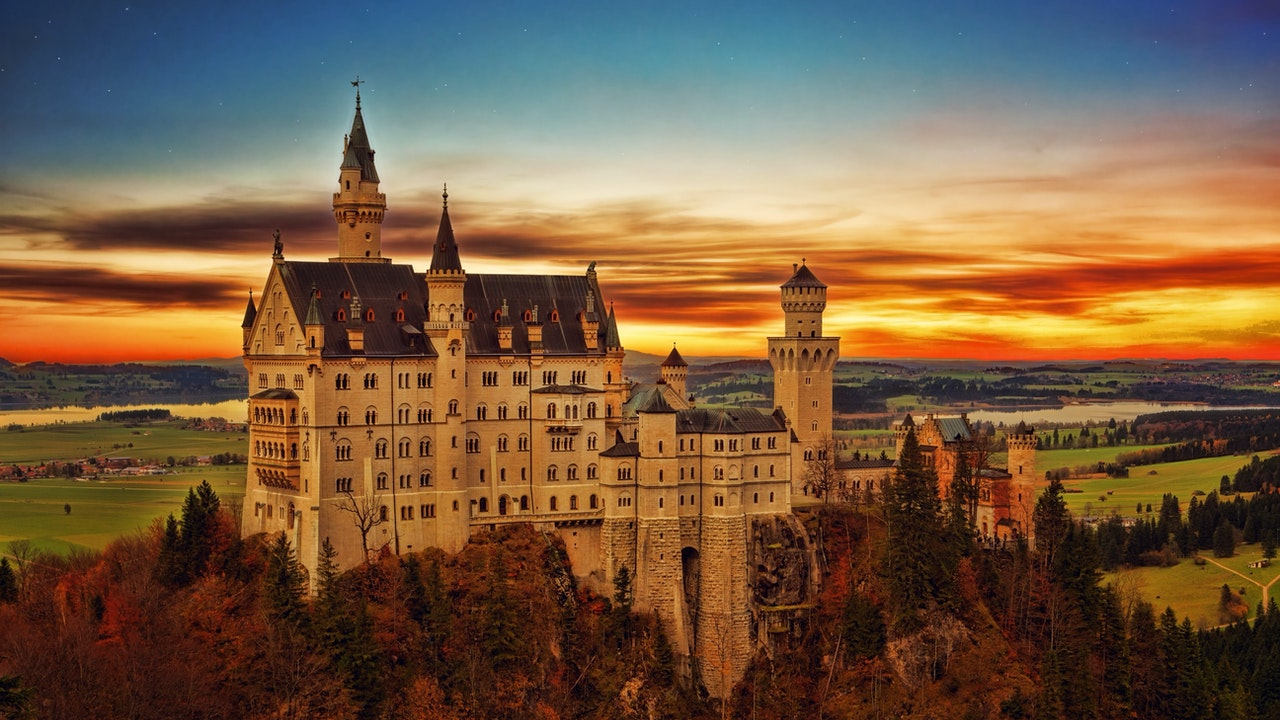
\includegraphics[scale=0.4]{images/general images/Arquitectura/arquitectura-gotica-imagenes.jpg}
      \caption{\small Comparación en la vida real}
    \end{figure}

        \begin{figure}[H]
      \centering
      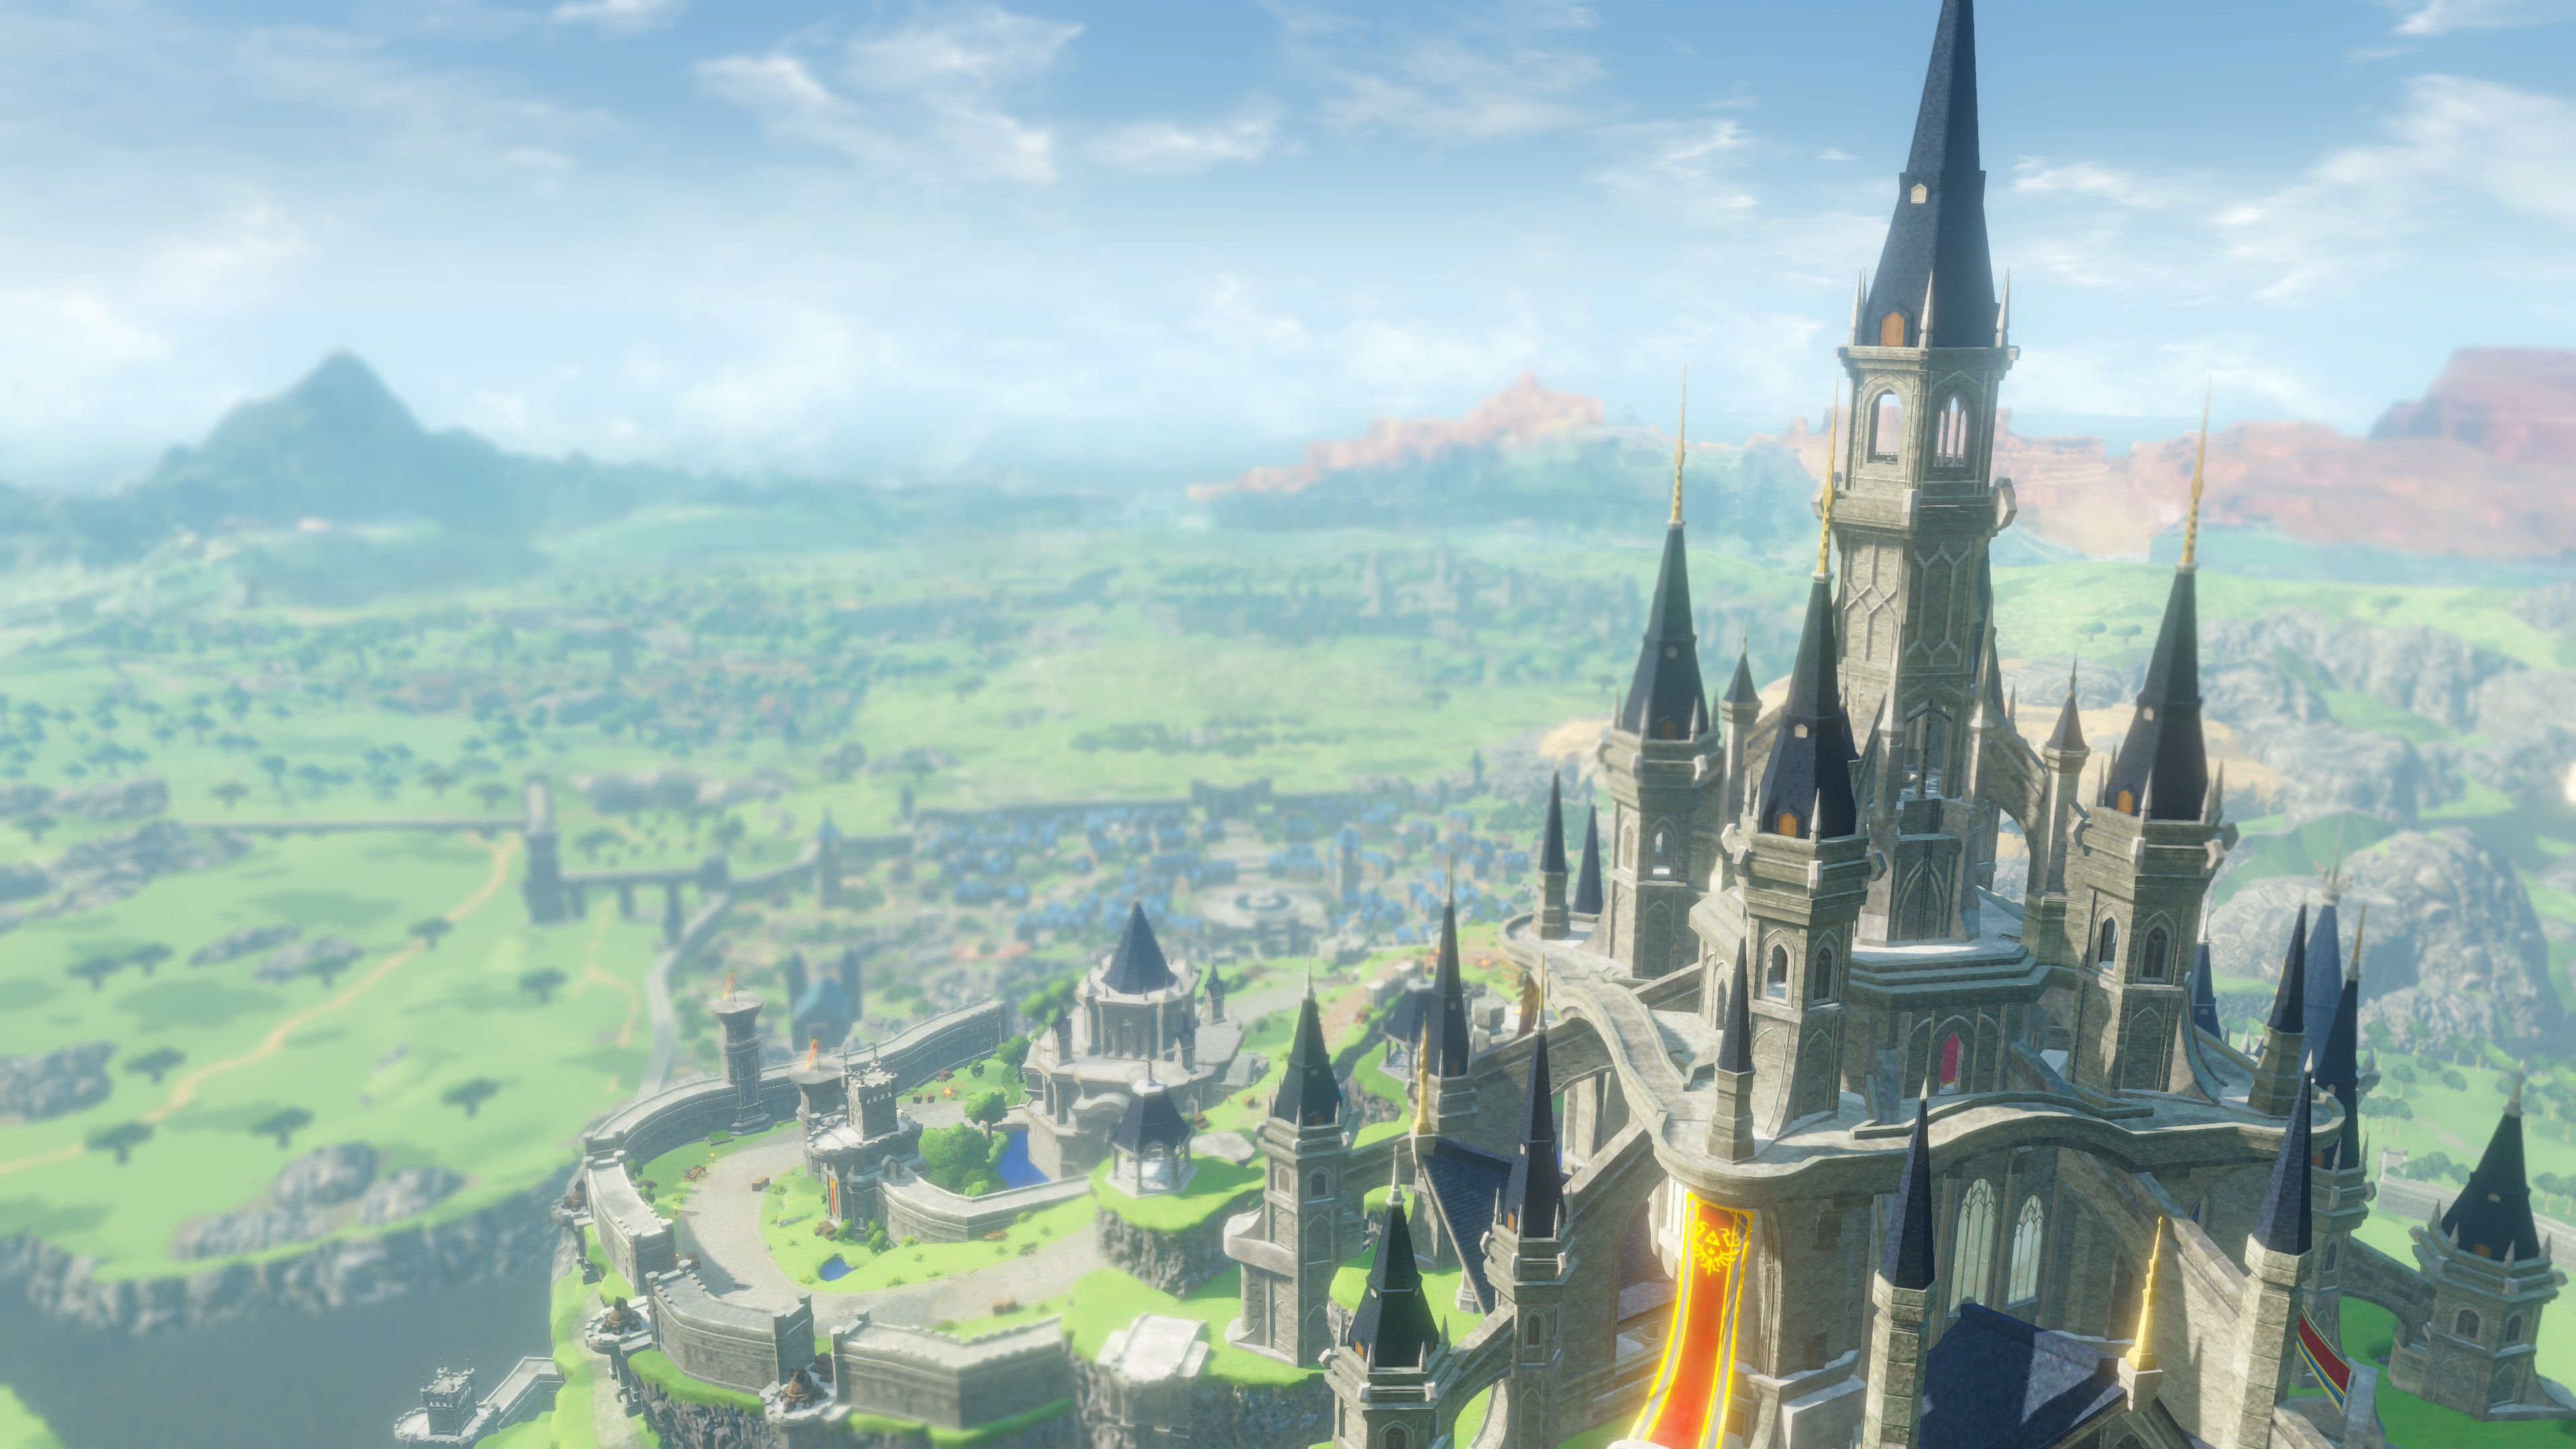
\includegraphics[scale=0.17]{images/general images/Arquitectura/castillo hyrule.jpg}
      \caption{\small Comparación dentro del juego}
    \end{figure}


\subsection{Arte}

Zelda Breath of the Wild utiliza el método de sombreado plano o mejor conocido como “cel shading”, el cual consiste en un tipo de renderización que tiene como objetivo hacer que los gráficos posean un estilo parecido a los dibujos hechos a mano. Esta técnica proviene de la animación tradicional, antes de la llegada de los métodos digitales, teniendo como resultado un estilo artístico realista en la iluminación y escenarios pero un estilo orientado más a la utilizada en la animación japonesa en cuanto se refiere a los personajes, en concreto, el estilo de Breath of the wild recuerda al estilo artístico empleado en las películas de studio Ghibli.

    \begin{figure}[H]
      \centering
      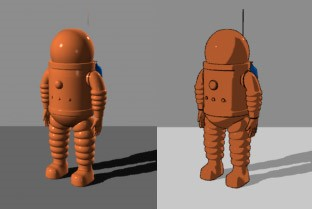
\includegraphics[scale=2]{images/general images/Pintura/celshading.jpg}
      \caption{\small Cel-shading primer ejemplo}
    \end{figure}

        \begin{figure}[H]
      \centering
      
\includegraphics[scale=0.4]{images/general images/Pintura/celshading2.jpg}
      \caption{\small Cel-shading segundo ejemplo}
    \end{figure}

\subsection{Fotografía}

La dirección fotográfica de un videojuego puede ser clave a la hora de transmitir las impresiones deseadas por parte de los desarrolladores al jugador. Concretamente en The Legend of Zelda: Breath of the Wild la fotografía cobra vital relevancia a la hora de enfatizar en la grandeza y extensión de Hyrule.
Ya desde un inicio se nos muestran secuencias de planos picados generales y tomas con gran profundidad de campo, que no dudan en apartar al personaje principal para dar protagonismo al mundo que lo rodea. Por otro lado, cuando se desea destacar y engrandecer algún elemento en concreto, se ve con frecuencia el uso de contrapicados.
En ciertos momentos en los que la atención del jugador tiene que centrarse en los propios personajes y sus diálogos, abundan los llamados planos americanos y los planos medios.
A la hora de mostrarnos hechos que sucedieron en el pasado, el videojuego también emplea filtros con texturas amarillentas características de la fotografía antigua.

\begin{figure}[H]
  \centering
  \begin{minipage}{0.4\textwidth}
    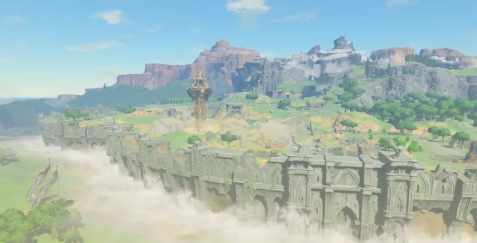
\includegraphics[width=\textwidth]{images/general images/Fotografia/Plano picado con gran profundidad de campo.png}
    \caption{3.3.1. Plano picado con gran profundidad de campo}
  \end{minipage}
  \hfill
  \begin{minipage}{0.4\textwidth}
    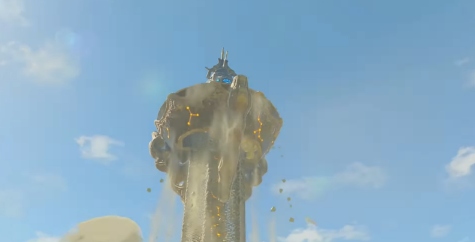
\includegraphics[width=\textwidth]{images/general images/Fotografia/Plano contrapicado.png}
    \caption{3.3.2. Plano contrapicado}
  \end{minipage}
\end{figure}

\begin{figure}[H]
  \centering
  \begin{minipage}{0.4\textwidth}
    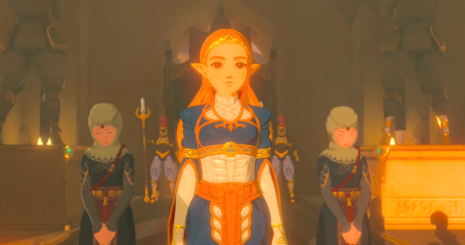
\includegraphics[width=\textwidth]{images/general images/Fotografia/Plano medio.png}
    \caption{3.3.3. Plano medio}
  \end{minipage}
  \hfill
  \begin{minipage}{0.4\textwidth}
    \includegraphics[width=\textwidth]{images/general images/Fotografia/Filtro amarillento similar a las fotografías antiguas.png}
    \caption{3.3.4. Filtro amarillento similar a las fotografías antiguas}
  \end{minipage}
\end{figure}



\subsection{La música}
Se tiene en cuenta que la mayoría de las travesías en la aventura, nos invade el silencio o los sonidos ambientales de los pájaros o más animales. Pero la música de ZBoW juega un gran papel en lo que es el game feel. Ya que en este juego a pesar de momentos puntuales no hace uso de grandes orquestas filarmónicas, sino de serenas melodías que nos ayudan a situarnos tanto geográficamente como temporalmente. Suaves flautas y oboes en la ciudad gerudo con el toque desértico que nos evocan a montañas de arena. Música con fuerte repercusión en la ciudad Goron, pero ninguna de estas opacando la acción del protagonista, si no más bien acompañándolo serenamente.

%-----------------------------------------------------------------
%-----------------------------------------------------------------

\newpage
\section{Análisis conceptual de imágenes}
    \hrule
\vspace{1cm}
    \subsection{1. Nerea}
    \begin{figure}[H]
      \centering
      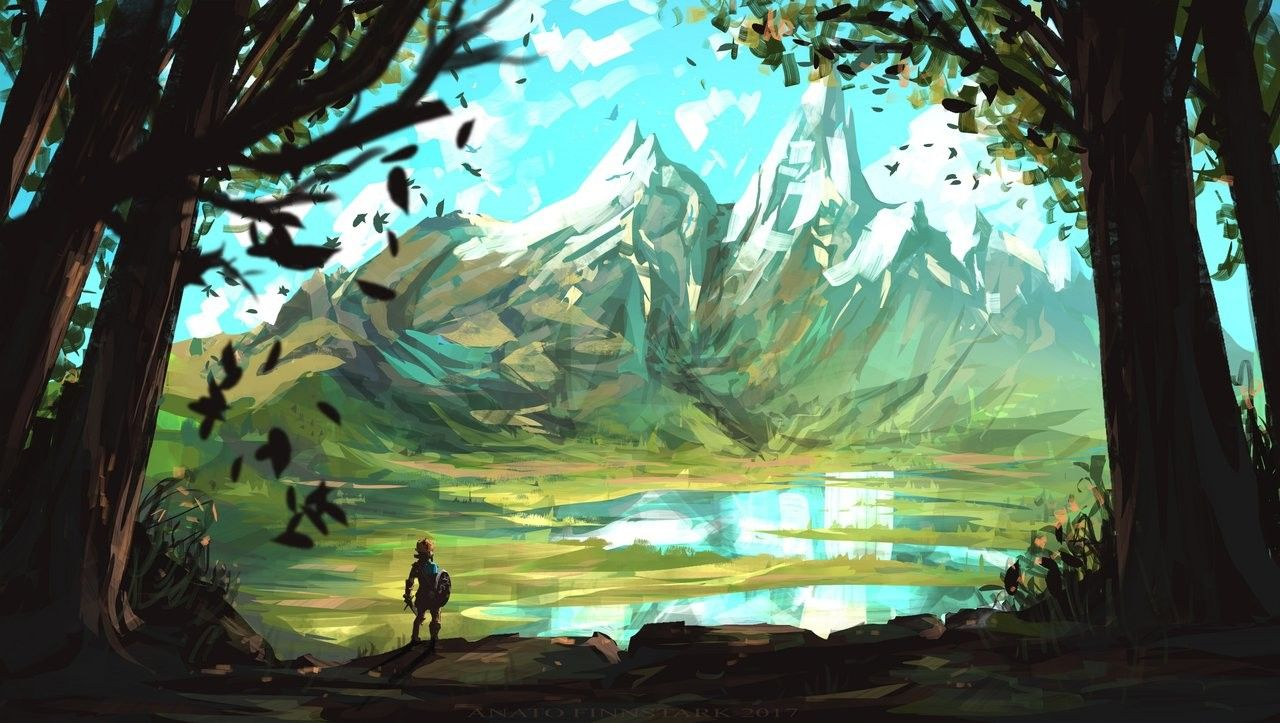
\includegraphics[width=\textwidth]{Nerea/1_concept_art.jpg}
      \caption{\small 4.1.1 Imagen}
    \end{figure}

    \begin{figure}[H]
      \centering
      \includegraphics[width=\textwidth]{images/Nerea/6_concept_art.png}
    \end{figure}
    Imagen compuesta por Link mirando hacía el vasto paisaje.

    
        \subsubsection{Análisis de la perspectiva}


    \begin{figure}[H]
      \centering
      \includegraphics[width=\textwidth]{Nerea/6_concept_art.png}
      \caption{\small 4.1.1.1 Línea del horizonte y tipo de vista}
    \end{figure}

    El vasto paisaje y límite fijado por el pie de una cordillera montañosa situada al fondo favorecen la clara visualización de una línea del horizonte que se encuentra en el centro, zona en la que el ojo humano tiende a enfocar primero en este tipo de ilustraciones. El tipo de vista es serena.
    debido a que todos los elementos presentes en la imagen son orgánicos, es imposible ubicar los puntos de fuga con claridad.


        \subsubsection{Análisis de la composición}

        
    \begin{figure}[H]
      \centering
      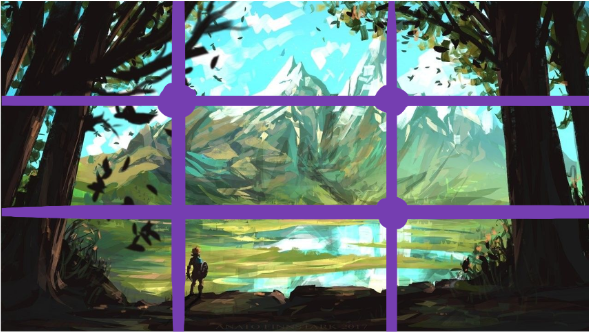
\includegraphics[width=\textwidth]{images/Nerea/Nerea Zelda concept 121.PNG}
      \caption{\small 4.1.2.1 Regla de los 2/3}
    \end{figure}

    Es posible discernir que la composición solo respira por la parte central inferior izquierda. Los árboles que ocupan ambos extremos de la imagen, junto con las montañas y el lago situados en el resto de puntos centrales, favorece a la riqueza en presencia de elementos y apoyos visuales. Aunque sean numerosos, no se consigue abrumar la vista del espectador ya que los puntos centrales se encuentran muy alejados y con mucha iluminación.

    \begin{figure}[H]
      \centering
      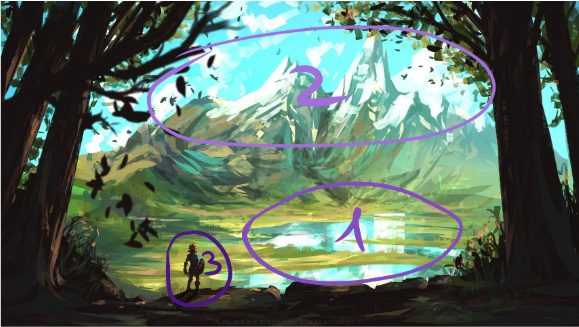
\includegraphics[width=\textwidth]{images/Nerea/Nerea Zelda concept 122.PNG}
      \caption{\small 4.1.2.2 Puntos de interés, principal y secundarios}
    \end{figure}

    Aunque pueda parecer que el principal punto de interés sean montañas, no llega a ser del todo cierto porque, aunque sea de grandes dimensiones en comparación con el resto de elementos, se demostrará en el siguiente apartado como la ruta visual acaba llegando al cristalino y extenso lago. En definitiva, tenemos a Link y la cordillera como puntos de interés secundarios y al lago como el principal.

    \begin{figure}[H]
      \centering
      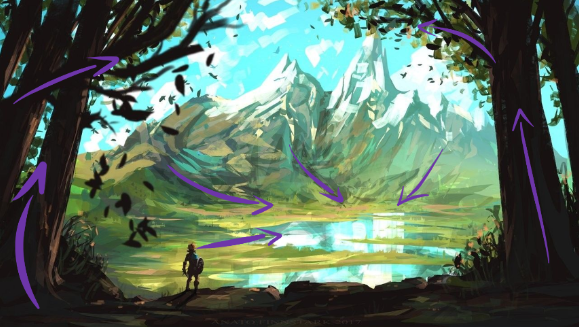
\includegraphics[width=\textwidth]{images/Nerea/Nerea Zelda concept 123.PNG}
      \caption{\small 4.1.2.3 Recorrido visual}
    \end{figure}

    El recorrido visual comienza principalmente en los árboles o la mirada de Link. La mirada de Link dirige nuestra vista directamente hacía el punto de interés principal, mientras que los troncos y abundantes ramas consiguen desplazar los ojos en dirección a las montañas cuyas laderas nos mandan terminantemente hacía el final de la ruta, que es el lago.

    \begin{figure}[H]
      \centering
      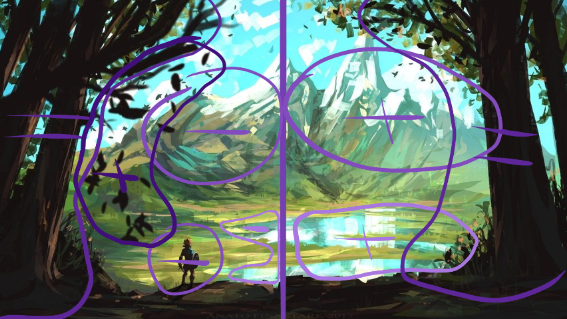
\includegraphics[width=\textwidth]{images/Nerea/Nerea Zelda concept 124.PNG}
      \caption{\small 4.1.2.4 Ley de la balanza, equilibrio de pesos y simetría vs. asimetría}
    \end{figure}

    La ilustración cumple la ley de la balanza ya que la presencia de diferentes elementos en la composición balancea el peso de todos ellos al completo. Los árboles de los extremos son prácticamente como reflejos iguales, neutralizando su peso. A su vez, a pesar de el gran volumen ocupado a la derecha por las montañas y parte del lago en comparación con los de la izquierda, la imagen se equilibra gracias a Link y unas copiosas hojas muy cercanas a nosotros con mucha saturación y poca luminosidad. Es por esto que la imagen, por ende, es simétrica. La buena combinación de tonalidades cálidas y frías a ambos extremos de la balanza.


        \subsubsection{Claroscuro}

        
    \begin{figure}[H]
      \centering
      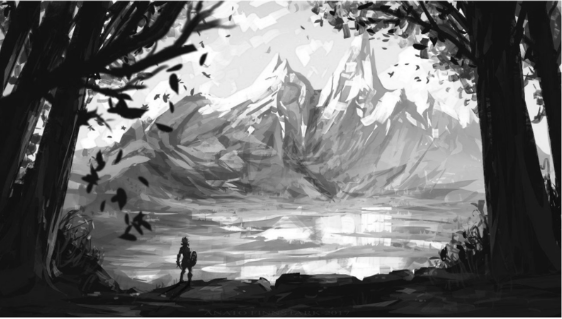
\includegraphics[width=\textwidth]{images/Nerea/Nerea Zelda concept 131.PNG}
      \caption{\small 4.1.3.1 Uso del claroscuro para representar la profundidad}
    \end{figure}

    Se pueden diferenciar claramente dos zonas, la primera y más cercana tiene los tonos muy oscuros, y la segunda siendo el paisaje montañoso con el lago que se extiende hacía el horizonte. Esta segunda tiene unos tonos mucho más luminosos y claros, por lo que gracias a este contraste se puede ver que al aplicar colores oscuros en el primer plano y unos con más luminosidad en el segundo, crea un efecto de profundidad.

    \begin{figure}[H]
      \centering
      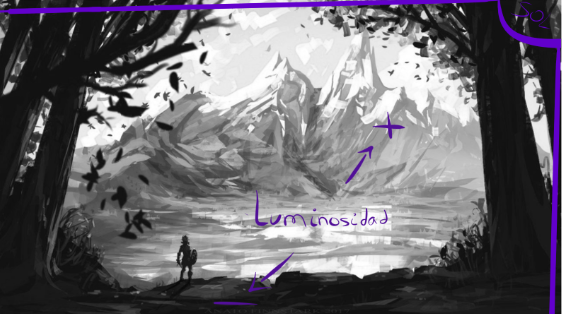
\includegraphics[width=\textwidth]{images/Nerea/Nerea Zelda concept 132.PNG}
      \caption{\small 4.1.3.2 Zonas más luminosas y menos, y ubicación de la fuente de iluminación}
    \end{figure}

    Como he comentado en el apartado anterior, las partes más luminosas serán las del segundo plano o fondo (zona clave alta) mientras que las menos iluminadas serán las del primero (zona clave baja). Gracias a la sombra de Link y árboles próximos, se puede saber que la fuente de iluminación (sol) se encuentra en la esquina superior derecha, conforme más nos alejemos menos será la luminosidad de los colores.

    \begin{figure}[H]
      \centering
      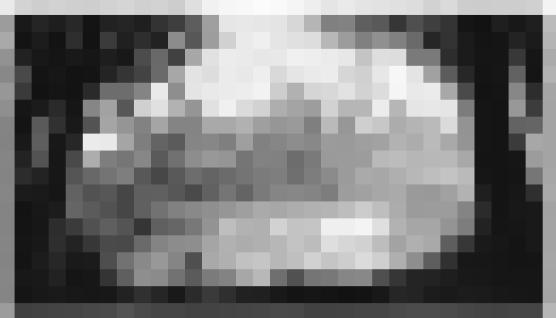
\includegraphics[width=\textwidth]{images/Nerea/Nerea Zelda concept 133.PNG}
      \caption{\small 4.1.3.3 Clave de la imagen}
    \end{figure}

    La clave de esta ilustración considero que es alta. Si bien hay una gran presencia de clave baja en los extremos y en la parte central izquierda hay una clave media, como podemos considerar que esta se acerca mucho a una clave alta y, si sumada con la clave alta de la zona superior y central derecha, es evidente asumir la fuerza de la clave alta que encima está colocada en zona de mayor relevancia e importancia visual.


        \subsubsection{Color}


    \begin{figure}[H]
      \centering
      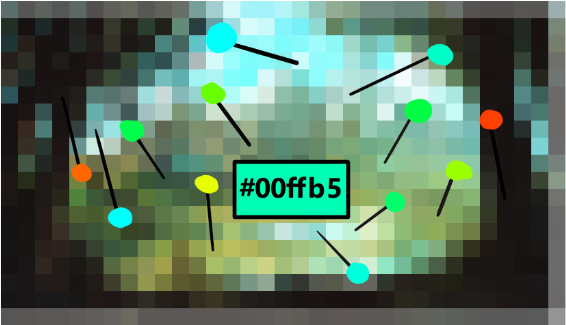
\includegraphics[width=\textwidth]{images/Nerea/Nerea Zelda concept 141.PNG}
      \caption{\small 4.1.4.1 Tonalidad de color global}
    \end{figure}

    Se tiene una tonalidad de color global fría pero no es su totalidad ya que, a su vez, vemos que se convive con colores de varias tonalidades (verdosas o amarillentras) y colores muy cálidos en los extremos de la imagen (árboles). Me he decantado por las tonalidades frías ya que, al ver el tono global resultante de los tonos situados al centro, he conseguido dar con un color azulado verdoso que no puede ser considerado del todo cálido, pero sí frío.

    \begin{figure}[H]
      \centering
      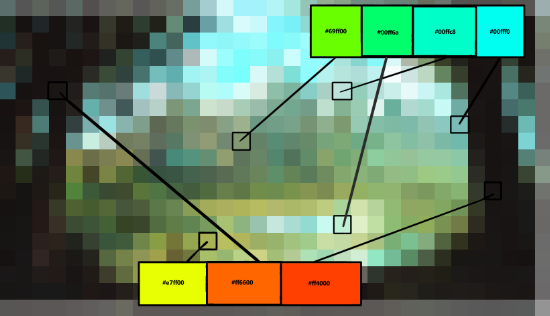
\includegraphics[width=\textwidth]{images/Nerea/Nerea Zelda concept 142.PNG}
      \caption{\small 4.1.4.2 Gama de color empleada}
    \end{figure}

    La gama de colores empleada en esta ilustración incluye una gama de tonalidades de amarillas/naranjas análogas (parte central inferior),  y otra gama de tonalidades de verdes/azules análogos (parte superior derecha). Haciendo justicia a la aclaración explicada en el apartado anterior, considero que la gama más importante y amplia es la de tonalidades verdes/azules análogas.

    \begin{figure}[H]
      \centering
      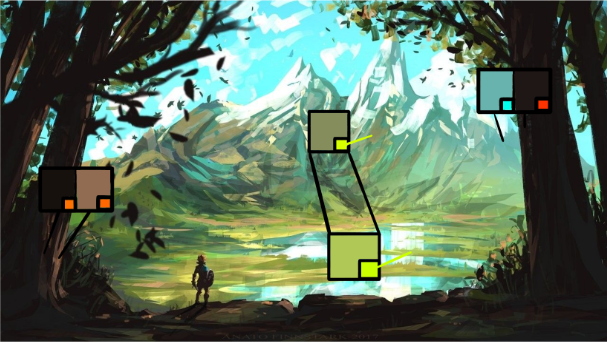
\includegraphics[width=\textwidth]{images/Nerea/Nerea Zelda concept 143.PNG}
      \caption{\small 4.1.4.3 Tipos de contraste}
    \end{figure}

    El contraste de luminosidad es la diferencia de luminosidad entre dos o más elementos visuales. Empleado para resaltar ciertos elementos variando la cantidad de luz/sombra aplicada o para conseguir un efecto de profundidad, En este caso he señalado dos tonalidades naranjas cuya luminosidad cambia en función del foco de luz y ayuda a representar las sombras proyectadas por este. En el contraste de saturación es posible discernir cambios en la intensidad de unos colores a otros, como por ejemplo el mostrado en el centro de la imagen, que son dos tonos verdosos prácticamente iguales que se encuentran saturados de diferente forma ya que las partes más cercanas deben estar más saturadas mientras las más alejadas deben estarlo mucho menos para conseguir profundidad. El contraste de tono está presente cuando, entre dos o más elementos visuales, es posible encontrar distinciones en cuanto a tono o matiz de sus respectivos colores. Esto ocurre entre colores cálidos y colores fríos, he señalado a la derecha los colores complementarios de la lejana ladera de la montaña y el tronco del árbol próximo a esta.

    \begin{figure}[H]
      \centering
      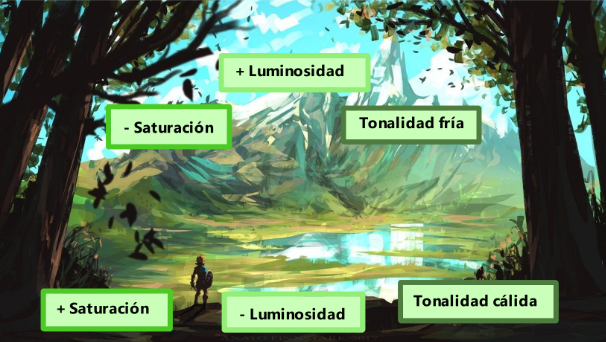
\includegraphics[width=\textwidth]{images/Nerea/Nerea Zelda concept 144.PNG}
      \caption{\small 4.1.4.4 Análisis de los colores empleados en primer y último plano}
    \end{figure}

    Es posible apreciar cómo los colores escogidos para el primer plano están muy saturados en comparación con los del fondo mientras que, a la hora de tener en cuenta la luminancia, el último plano tiene colores con mucha más luminosidad que los del primer plano. En cuanto a la tonalidad, con el fin de representar la profundidad, se usan tonos cálidos en el primer plano y fríos en el último.
        \newpage

%-----------------------------------------------------------------
%-----------------------------------------------------------------

    \subsection{2. Jesús}

        \begin{figure}[H]
          \centering
          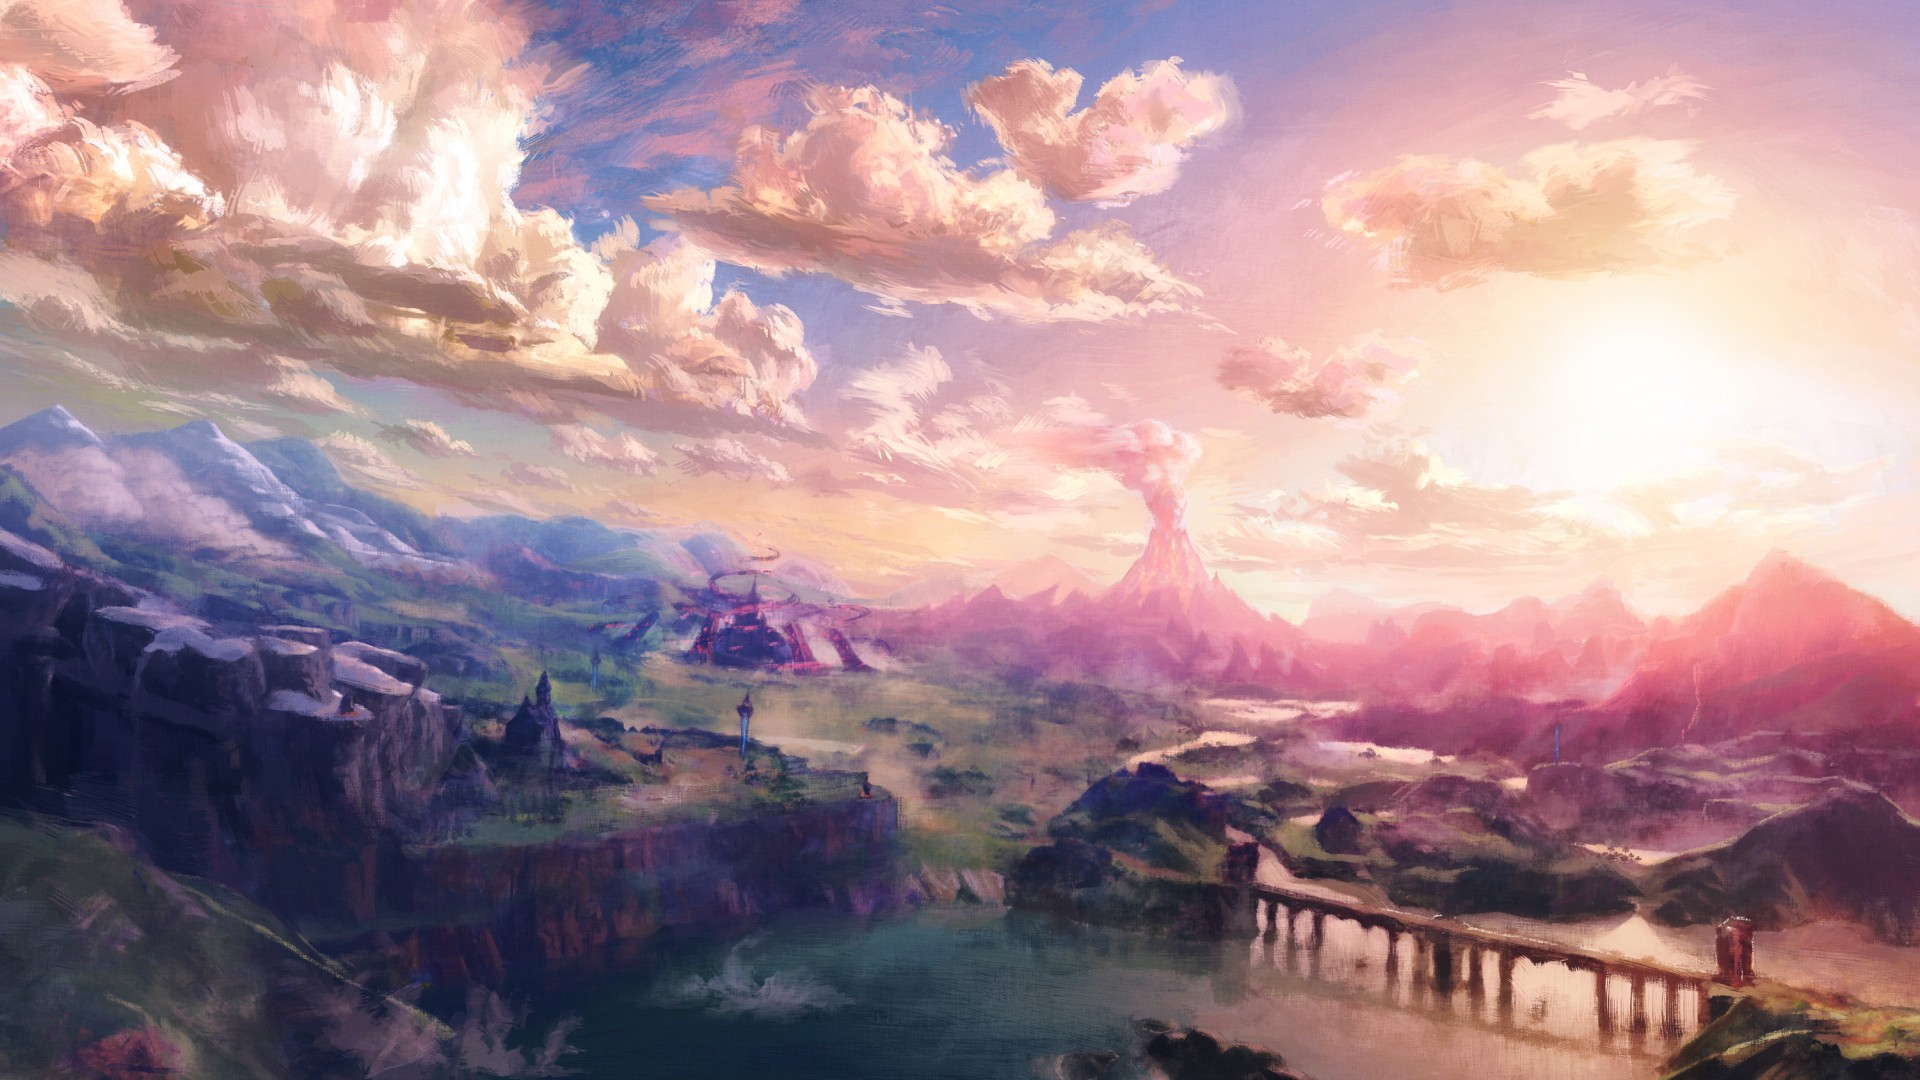
\includegraphics[width=\textwidth]{images/Concepts/2_concept_art.jpg}
          \caption{\small{4.2 Imagen}}
        \end{figure}
        
        Esta imagen se trata de un concept art oficial del juego, en el que se puede apreciar dos puntos importantes del juego, el castillo de Hyrule y el volcán al fondo. 

        \subsubsection{Perspectiva}
        \begin{figure}[H]
          \centering
          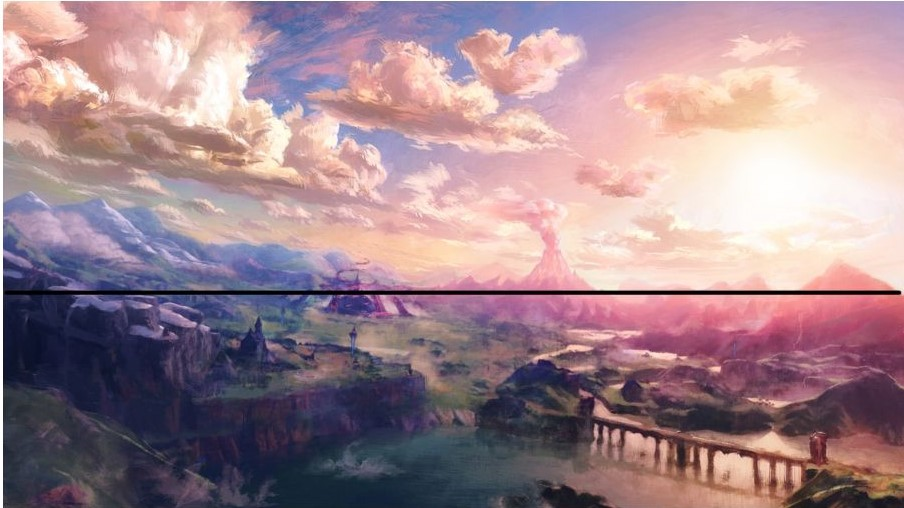
\includegraphics[width=\textwidth]{Jesus/Seccion2/Group 4.JPEG}
          \caption{Línea de Horizonte}
        \end{figure}

        La línea de horizonte se sitúa en prácticamente el centro de la imagen, tratándose de una imagen en vista serena. 

        \newpage

        \begin{figure}[H]
          \centering
          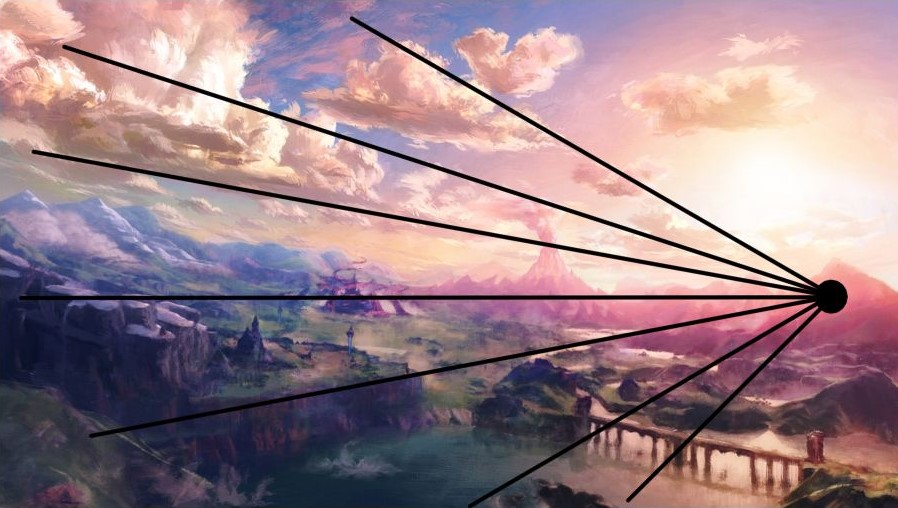
\includegraphics[width=\textwidth]{images/Jesus/Seccion2/Group 3.JPEG}
          \caption{Puntos de fuga}
        \end{figure}
        Al ser una composición muy orgánica, no es posible discernir un punto de fuga claro. Aun así, se puede discernir un "punto de fuga" falso. Es decir, podemos usar el sol como un punto de fuga, ya que como he explicado anteriormente, la imagen crea líneas que se forman creando cierta perspectiva.

        \newpage

        
        \subsubsection{Composición}
        
          \begin{figure}[H]
            \centering
            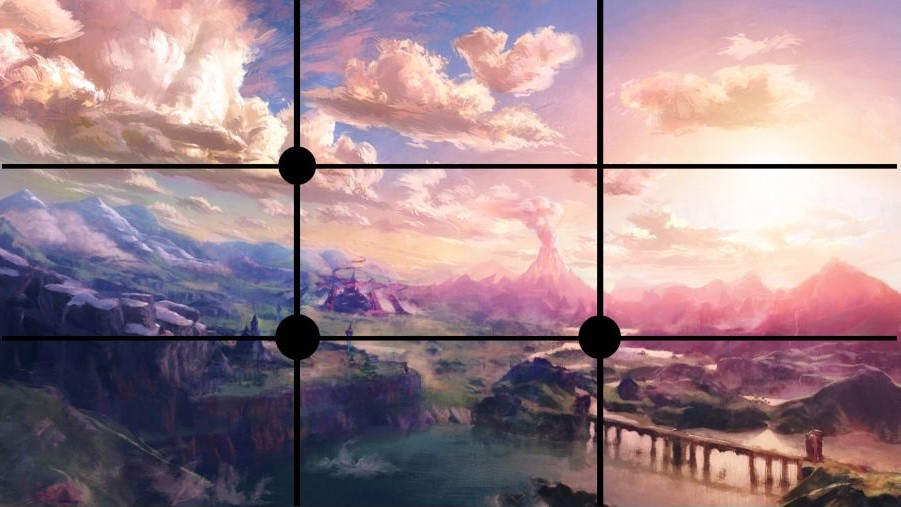
\includegraphics[width=\textwidth]{images/Jesus/Seccion2/Group 1.JPEG}
            \caption{Regla de tres tercios}
          \end{figure}
          
          La regla de los tres tercios sitúa los puntos principales en los tercios superior e inferior izquierdos y el tercio inferior derecho. 
          Siendo estos puntos de interés donde recae la atención del espectador, que precisamente son también los puntos más importantes de la imagen.
          \newpage
          \begin{figure}[H]
            \centering
            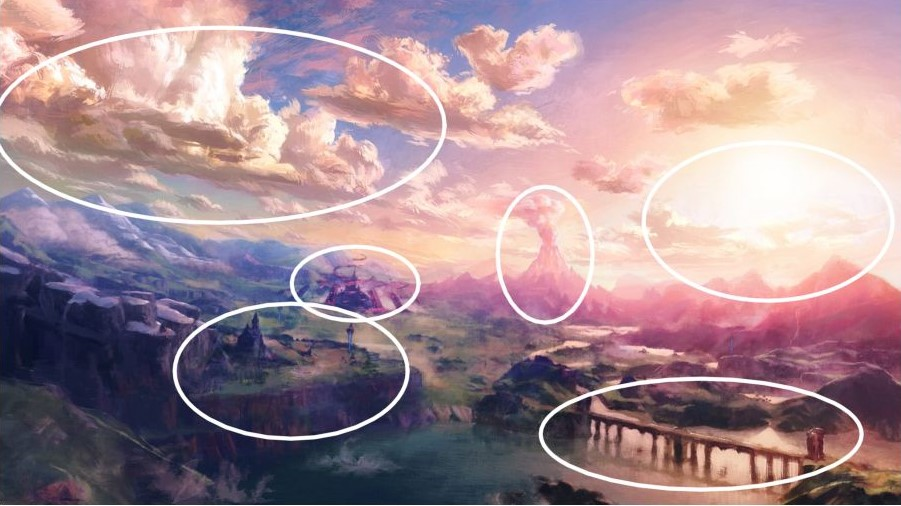
\includegraphics[width=\textwidth]{images/Jesus/Seccion2/Group 5.JPEG}
            \caption{\small {Puntos de Interés}}
          \end{figure}
          Hay muchos puntos de interés a destacar en esta imagen. Donde podemos decir que uno de los puntos más destacables son el sol, el cual ilumina del resto de los puntos.
          Después se destacan muchos las nubes debido a que ocupan gran parte de la composición. 
          También se destacan mucho el volcán debido a que hace contraste de colores entre el fondo y el castillo de Hyrule. 

          Para finalizar con los puntos de interés, se destacan el puente a la derecha debido a que sitúa en el lago, el cual contrasta el color claro junto al color oscuro del puente, y la meseta situada a la izquierda, que es donde Link empieza su aventura.
          
         \newpage
          \begin{figure}[H]
            \centering
            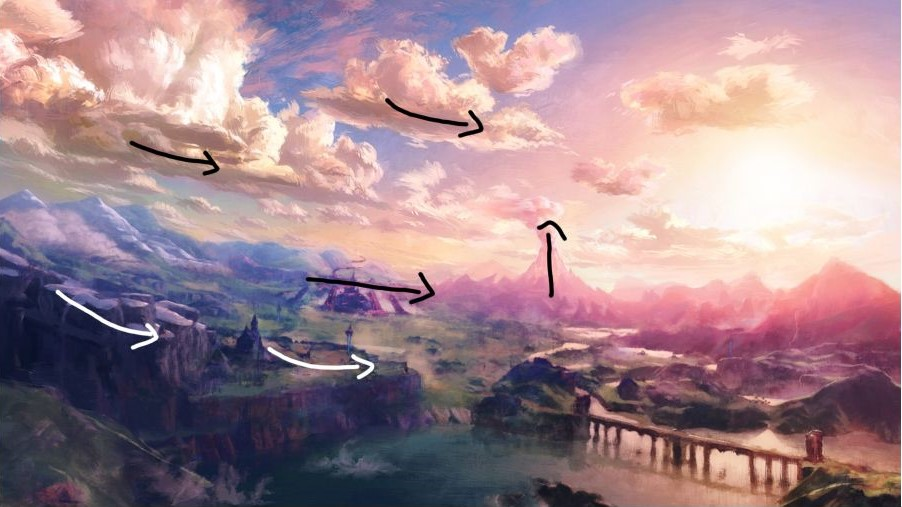
\includegraphics[width=\textwidth]{images/Jesus/Seccion2/Group 2.JPEG}
            \caption{Recorridos visuales}
          \end{figure}
          En cuanto a los recorridos visuales, podemos decir que prácticamente la imagen lleva al espectador hacia la derecha, siendo más específico, el sol. 
          Siendo las nubes uno de los recorridos más claros, ondeándose hacia el sol, incluyendo en esta “onda de movimiento” la meseta y el escenario; terminando en las montañas, las cuales se representan de forma más estática, indicando el final de la imagen. 

          Es más, se puede apreciar como la imagen es muy estática en la parte derecha, reforzando la teoría de que la imagen se comporta como una ola que te lleva hacia la parte derecha de la imagen.
          \newpage

          \begin{figure}[H]
            \centering
            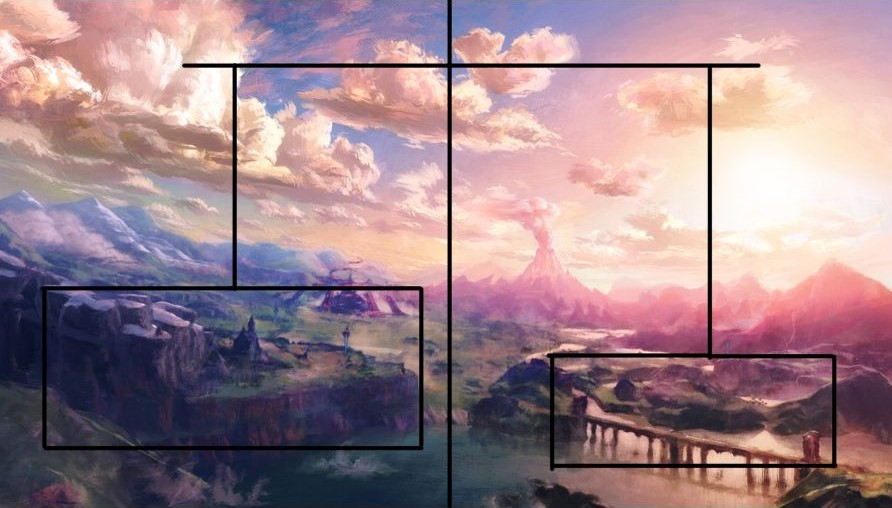
\includegraphics[width=\textwidth]{Jesus/Seccion2/Group 6.JPEG}
            \caption{Ley de la balanza}
          \end{figure}
          
          La ley de la balanza nos indica que el peso de la imagen tiene cierto desequilibrio, acentuándose en la parte izquierda de la imagen.
          Aunque tampoco podemos decir que todo el peso recae en la parte derecha de la imagen debido a que una parte importante de la imagen recae en la parte de derecha de esta misma. 

          Y para terminar, la simetría es nula en esta imagen debido a que primero, es una composición orgánica y la simetría no suele estar presente en este tipo de composiciones; y segundo, la ley de pesos se reparte por toda la imagen. 
          \newpage
        \subsubsection{Claroscuro}
          \begin{figure}[H]
            \centering
            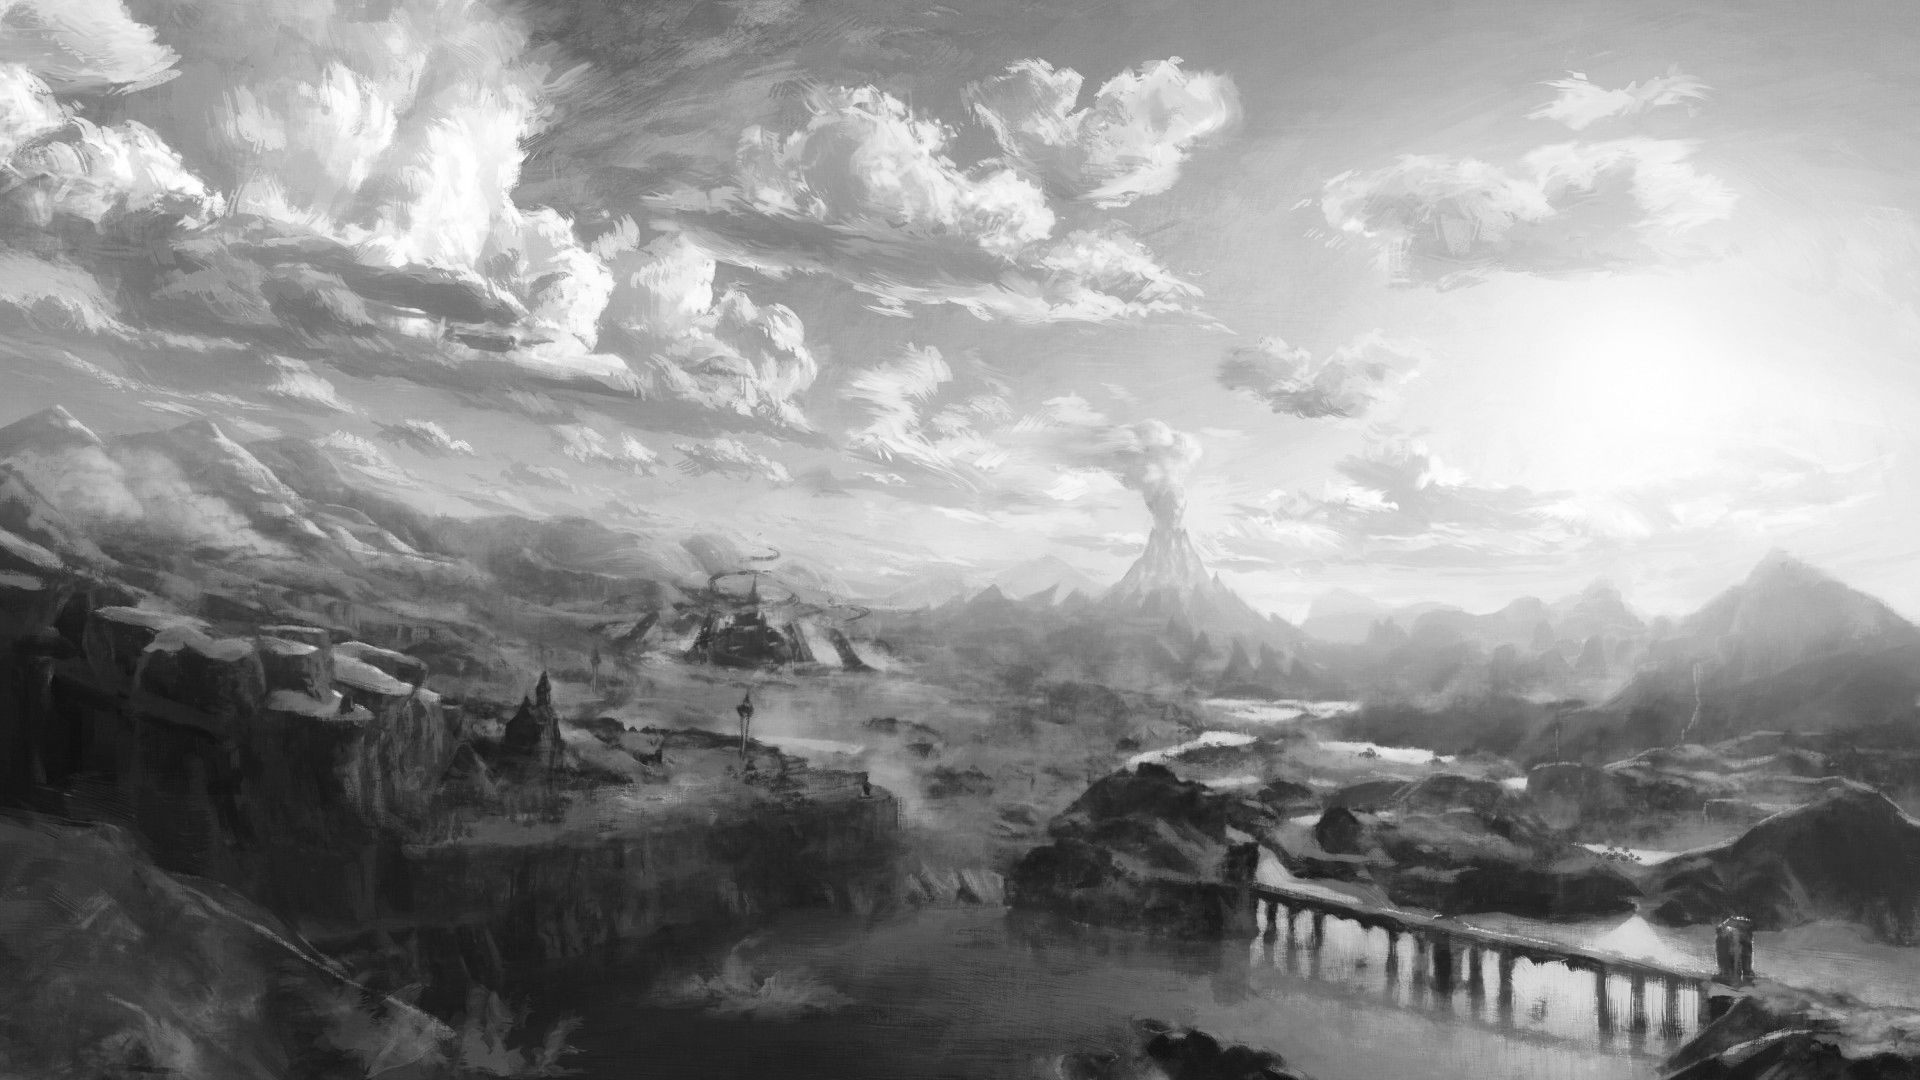
\includegraphics[width=\textwidth]{Jesus/Seccion2/Clarocuro.jpg}
            \caption{Claroscuro}
          \end{figure}

          Pasando la imagen a claroscuro se puede discernir su profundidad de forma muy clara, separando el cielo de la tierra muy efectiva. 
          La parte de la tierra tiene una clave más baja mientras que el cielo dispone de una clave mucho más alta al estar más iluminada. 
          \newpage
          \begin{figure}[H]
            \centering
            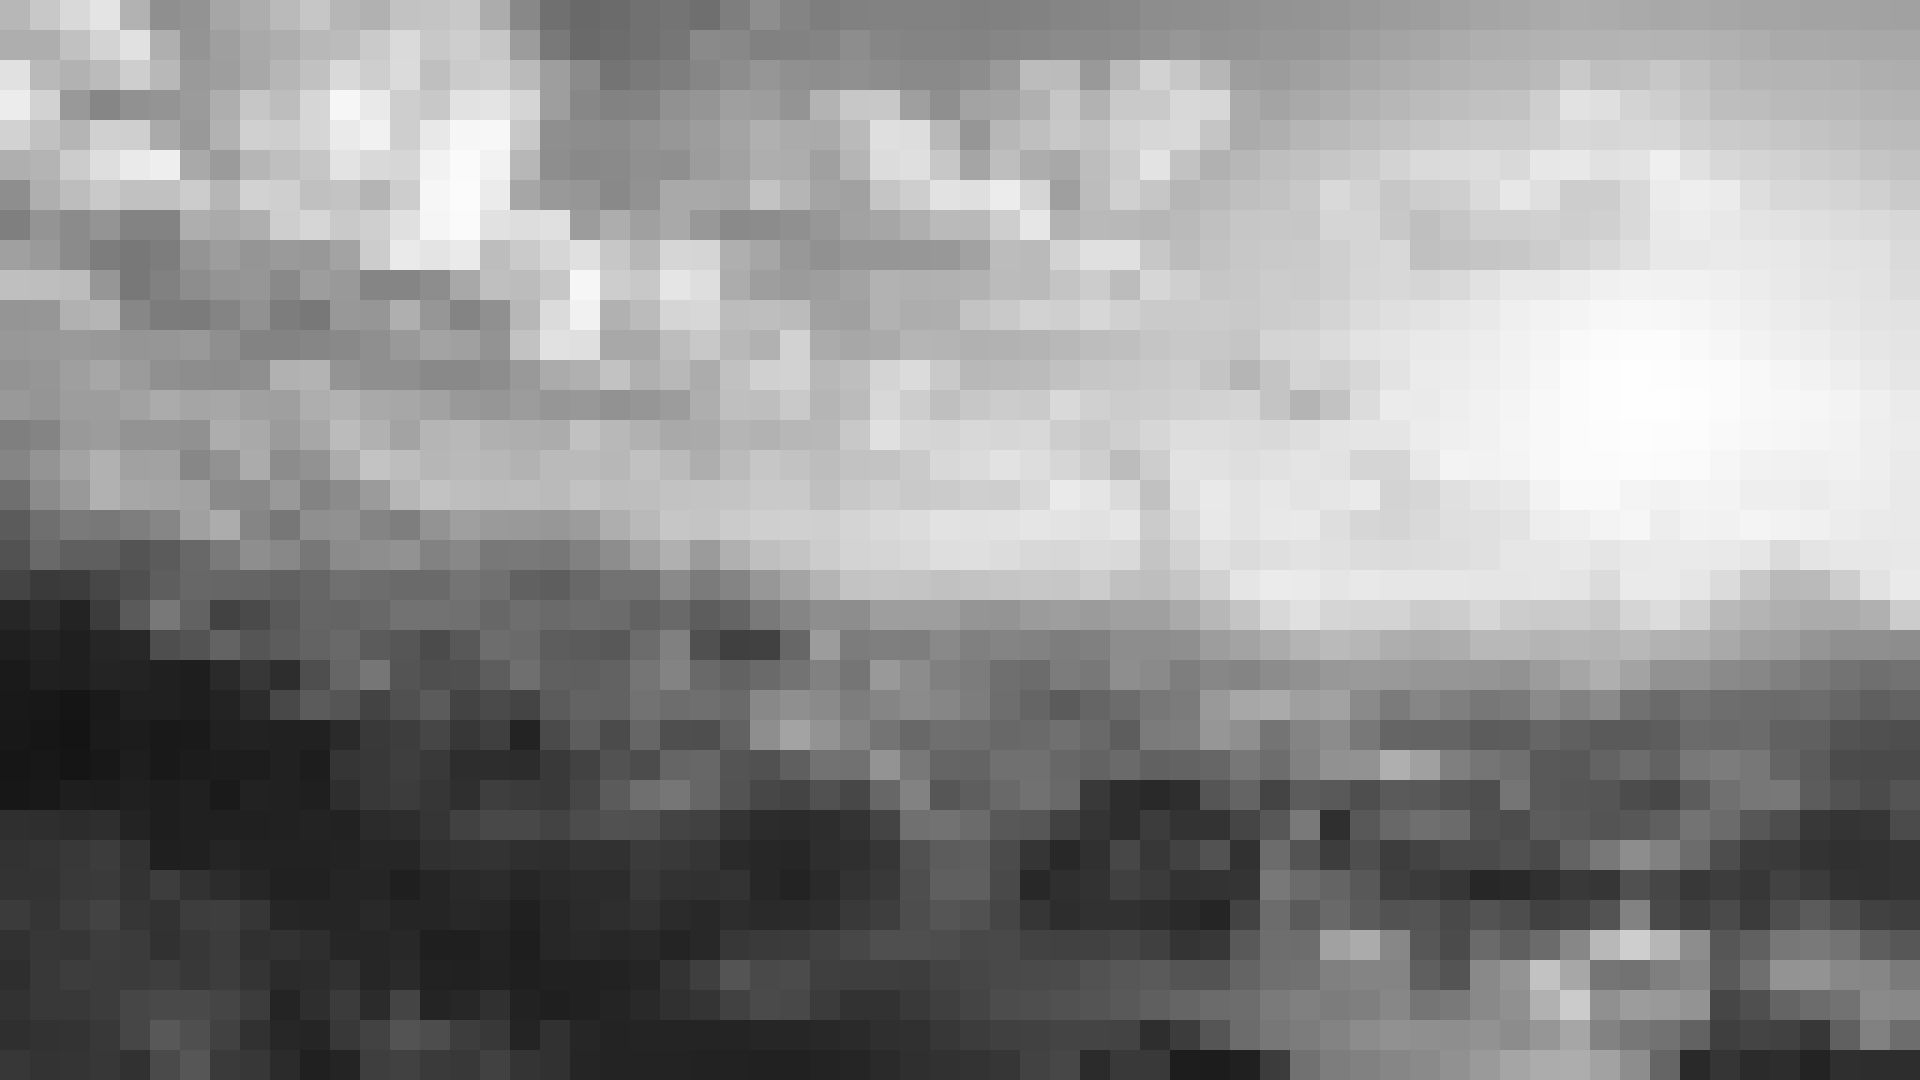
\includegraphics[width=\textwidth]{Jesus/Seccion2/pixel.jpg}
            \caption{Claroscuro en pixeles}
          \end{figure}
          Si pixelizamos el claroscuro, se puede discernir aún más la separación entre cielo y tierra mencionada anteriormente. 
          \newpage
          \begin{figure}[H]
            \centering
            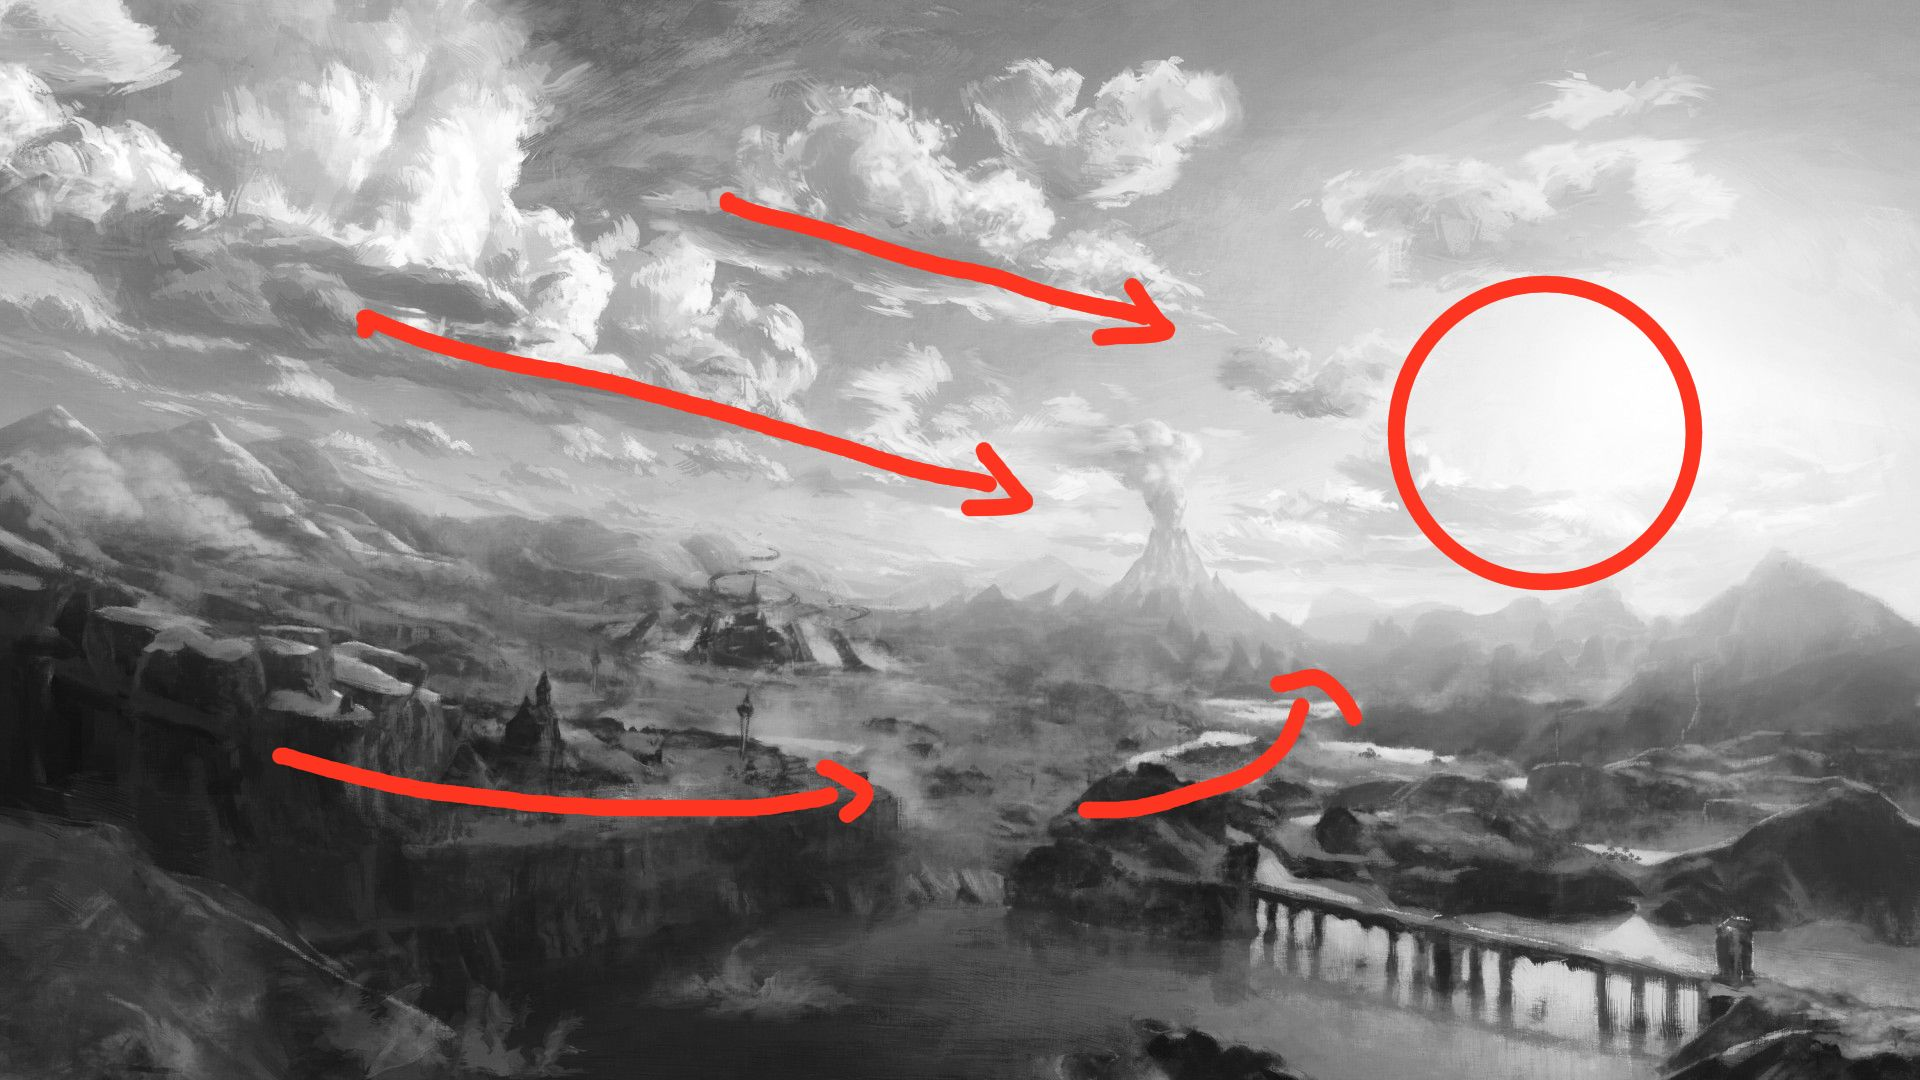
\includegraphics[width=\textwidth]{Jesus/Seccion2/Clarocuro con recorridos.jpg}
            \caption{Claroscuro con recorrido de luminosidad}
          \end{figure}
          Debido a que la fuente de luz de la imagen procede del sol, el recorrido hacia la fuente es muy parecido a los recorridos visuales. 
          \newpage

        \subsubsection{Color}
        
          \begin{figure}[H]
            \centering
            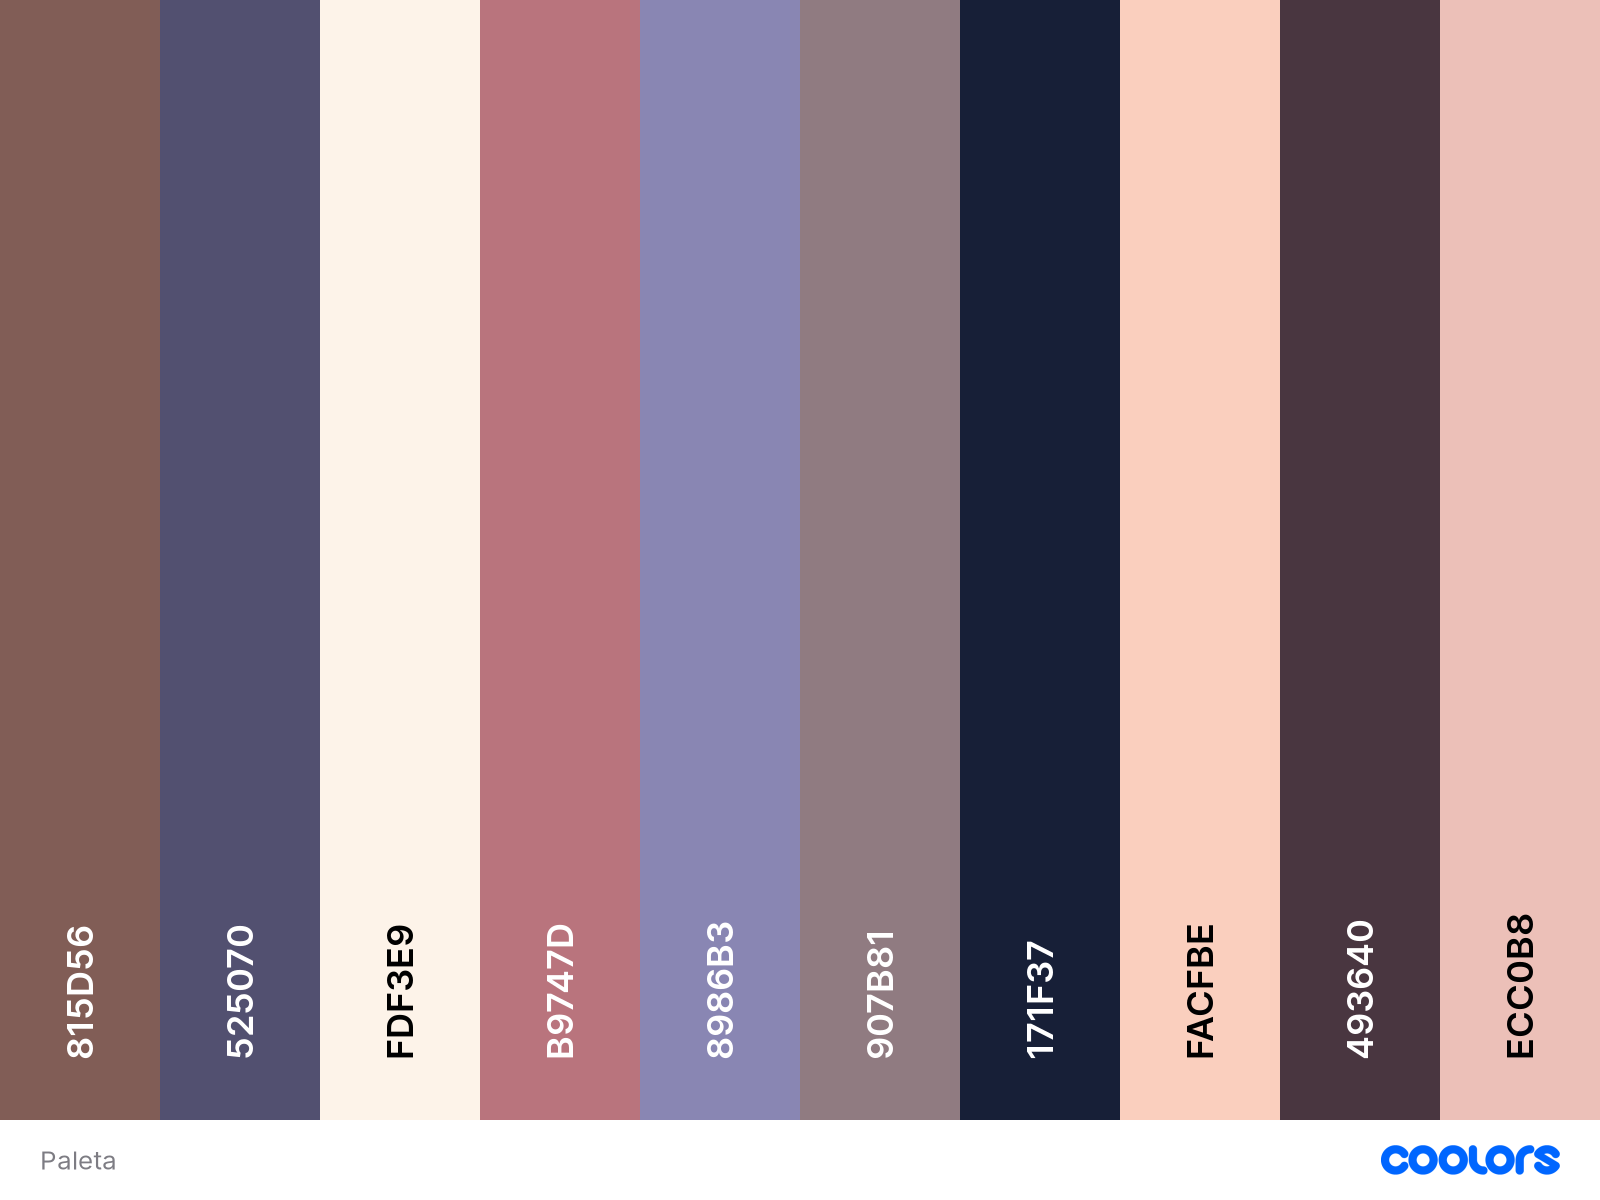
\includegraphics[width=\textwidth]{Jesus/Seccion2/Paleta.png}
            \caption{Paleta de colores}
          \end{figure}
          Si extraemos la paleta de colores, se puede apreciar que la imagen se compone de colores análogos, usando el rosa, el amarillo y el azul principalmente, y el verde color secundario. 
          
          \newpage
          
          \begin{figure}[H]
            \centering
            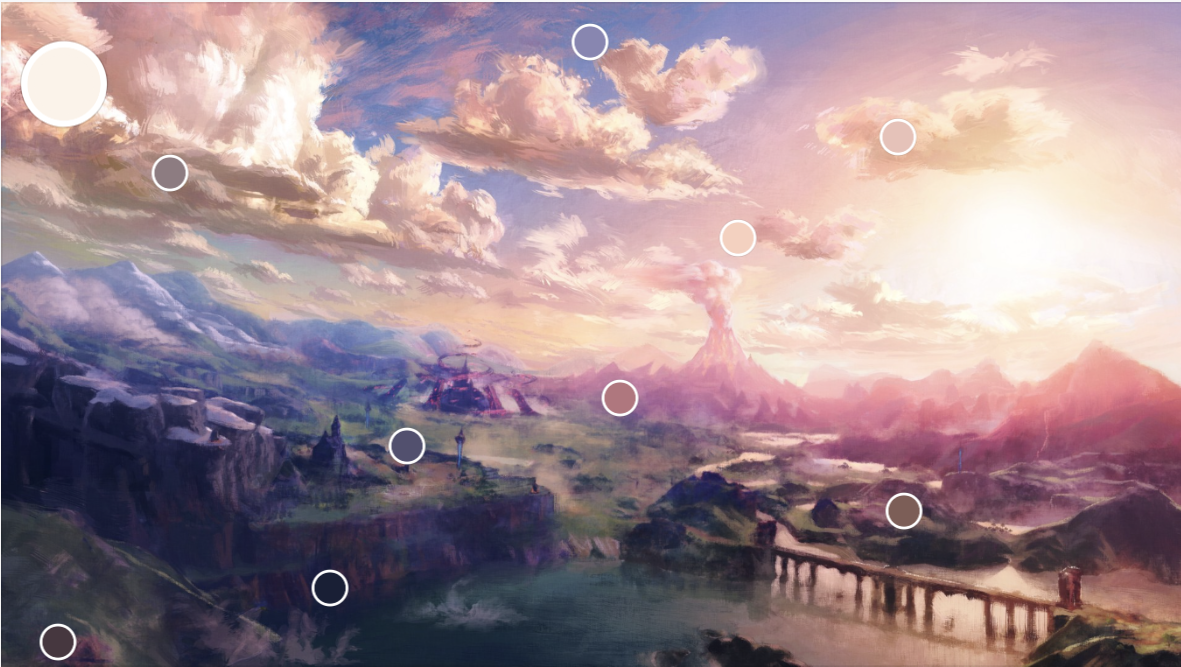
\includegraphics[width=\textwidth]{Jesus/Seccion2/Tonalidad.png}
            \caption{Paleta de colores}
          \end{figure}
          Con la tonalidad de la imagen se puede apreciar la gran cantidad de colores diferentes de los que dispone la imagen. Aunque se puede destacar el uso de colores cálidos en toda la composición, usando fríos solamente en un poco de la hierba del suelo y el cielo. 
          
          \newpage

          \begin{figure}[H]
            \centering
            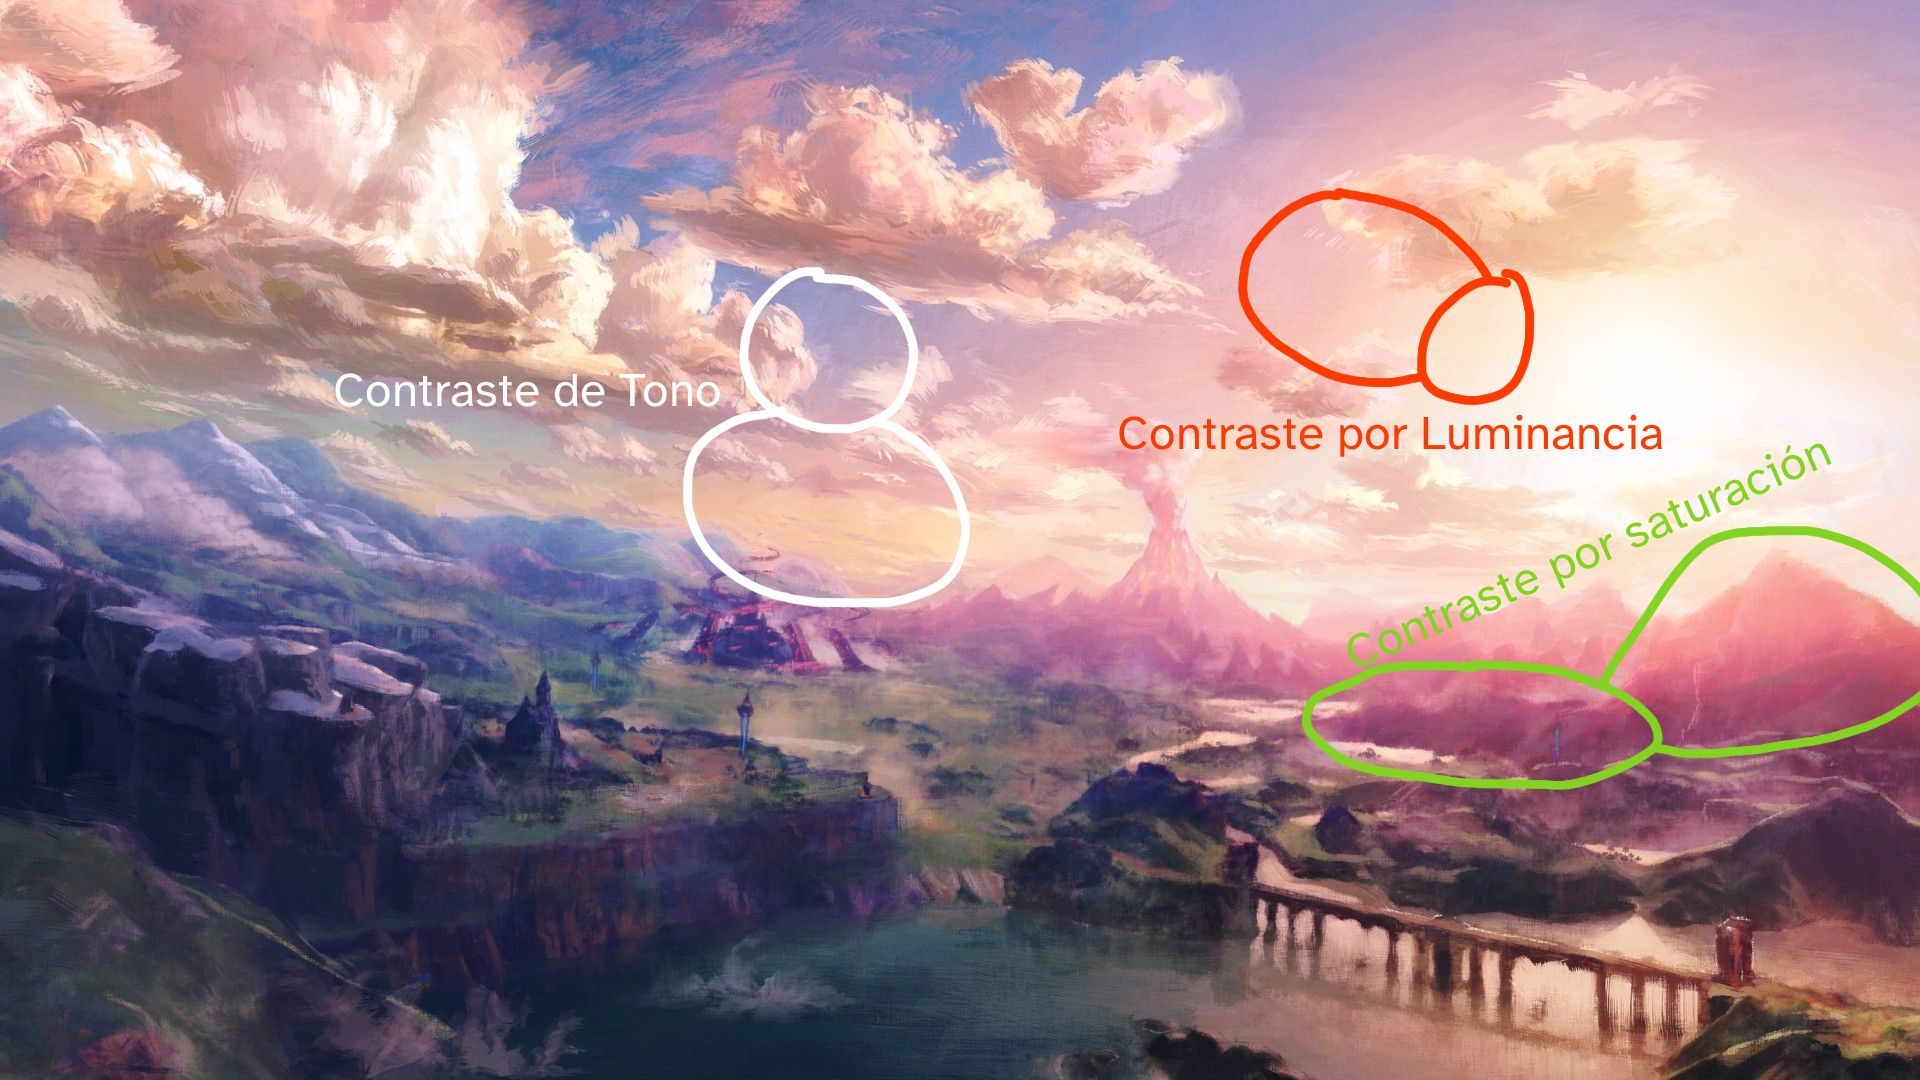
\includegraphics[width=\textwidth]{Jesus/Seccion2/contrastes.jpg}
            \caption{Contrastes}
          \end{figure}

          Se pueden hallar muchos tipos de contrastes en esta imagen. 

          El contraste de saturación se usa en las montañas para diferenciar las montañas pequeñas o más alejadas con una saturación rosácea más clara mientras que las montañas más cercanas usan una saturación más elevada. 

          El contraste de luminancia se usa principalmente en el cielo para diferencias los diferentes tonos de color que hay en el cielo. Se usa un amarillo muy brillante en el sol y se baja progresivamente la luminancia haciendo efecto de halo. 

          El contraste de tono se usa en el cielo, destacando el uso del azul y el amarillo haciendo un contraste muy fuerte, ya que ambos son opuestos en la rueda de color. 

          \newpage

%-----------------------------------------------------------------
%-----------------------------------------------------------------

    \subsection{3. Saul}
    \begin{figure}[H]
      \centering
      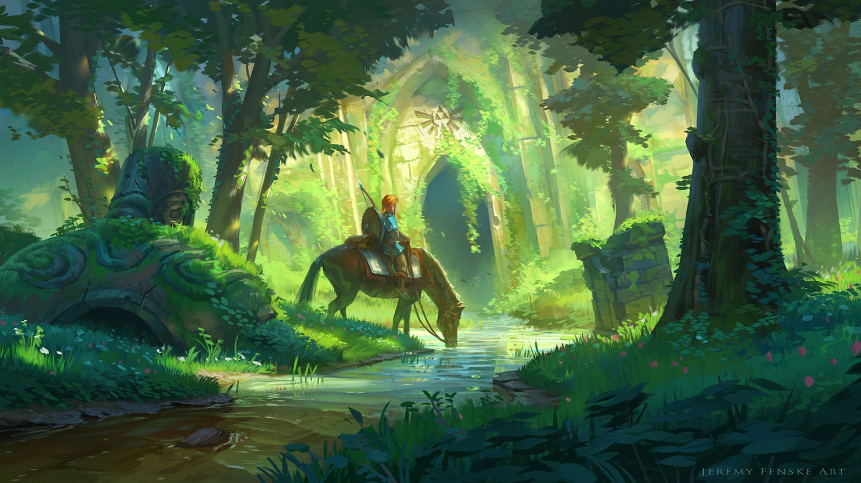
\includegraphics[width=\textwidth]{images/Saúl/Sección 3/EA_img3_0Main.png}
      \caption{\small 4.3.3. Imagen}
    \end{figure}
    Se trata de una imagen oficial del juego, y se compone por el personaje principal montado a su caballo Epona.

    
        \subsubsection{Análisis de la perspectiva}


    \begin{figure}[H]
      \centering
      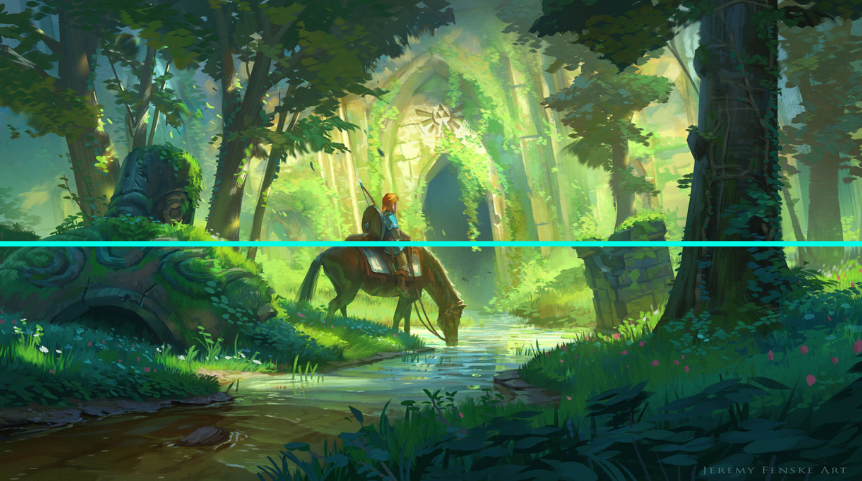
\includegraphics[width=\textwidth]{images/Saúl/Sección 3/EA_img3_1Perspectiva_1LineaTierra-TipoVista.png}
      \caption{\small 4.3.1.1 Línea del horizonte y tipo de vista}
    \end{figure}

    La línea del horizonte se halla sobre una altura media e incluso si afinamos mucho se puede apreciar que está ligeramente desplazada hacia arriba. Como la línea del horizonte se encuentra en la zona central de la ilustración podemos afirmar que estamos ante una vista serena.

    \begin{figure}[H]
      \centering
      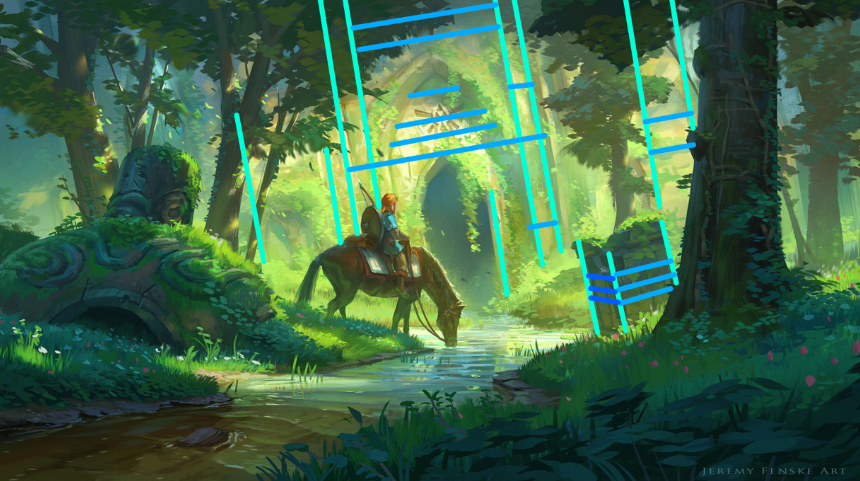
\includegraphics[width=\textwidth]{images/Saúl/Sección 3/EA_img3_1Perspectiva_2PuntosFuga.png}
      \caption{\small 4.3.1.2 Puntos de fuga}
    \end{figure}

    Aunque en la mayoría de la imagen predomina la naturaleza al fondo se puede apreciar un antiguo edificio en el cual podemos encontrar hasta dos puntos de fuga, ya que solo vemos una fachada y está algo inclinada. Además si nos fijamos bien, más adelante encontramos una ruina de una columna en la que sí se puede llegar a apreciar los tres puntos de fuga. Sin embargo en el resto de la imagen no se pueden apreciar más puntos de fuga, ya que como he dicho antes predomina la naturaleza.
(Estos puntos de fuga están todos fuera de la ilustración por lo que se han marcado con distintos colores las líneas que irían al punto de fuga, pero no se han alargado en todos los casos para no entorpecer a la vista).


        \subsubsection{Análisis de la composición}

        
    \begin{figure}[H]
      \centering
      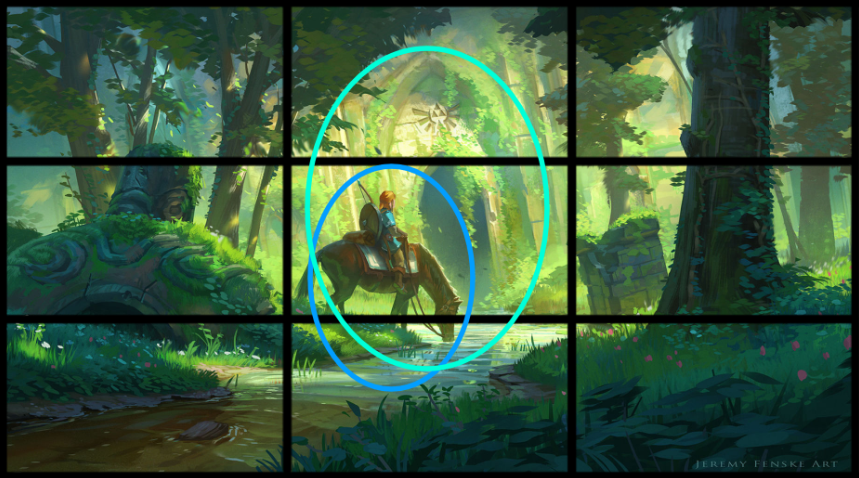
\includegraphics[width=\textwidth]{images/Saúl/Sección 3/EA_img3_2Composicion_1Regla2-3.png}
      \caption{\small 4.3.2.1 Regla de los 2/3}
    \end{figure}

En esta ilustración podemos apreciar como los elementos principales se encuentran en el centro de la imagen. Además como podemos ver el personaje principal está contenido en la sección del centro de esta regla de los 2/3.

    \begin{figure}[H]
      \centering
      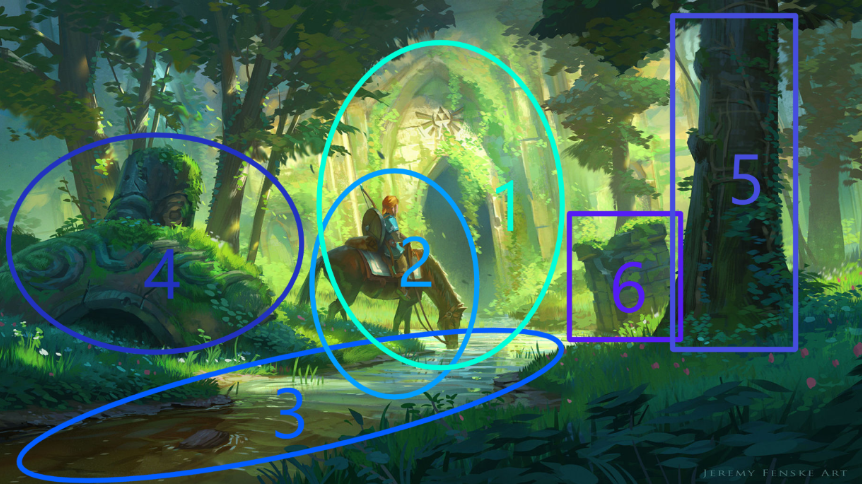
\includegraphics[width=\textwidth]{images/Saúl/Sección 3/EA_img3_2Composicion_2PuntosInteres.png}
      \caption{\small 4.3.2.2 Centro de interés, principal y secundarios}
    \end{figure}

Los principales puntos de interés son en primer lugar el templo al que le está lloviendo toda la luz de la imagen indicando que este es uno de los elementos más importantes y en segundo lugar es Link el personaje principal con el caballo quedándose con algo de esa luz que recibe el primer punto de interés, luego ya como puntos de interés secundarios tenemos en tercer lugar el río marcando un poco la ruta visual tema que trataremos ahora en la siguiente diapositiva, luego ya tenemos en el cuarto círculo un guardián y luego ya el quinto punto con el árbol ocupando la parte de la derecha de la ilustración y por último casi sin importancia las ruinas de la columna que corresponde al sexto punto de interés

    \begin{figure}[H]
      \centering
      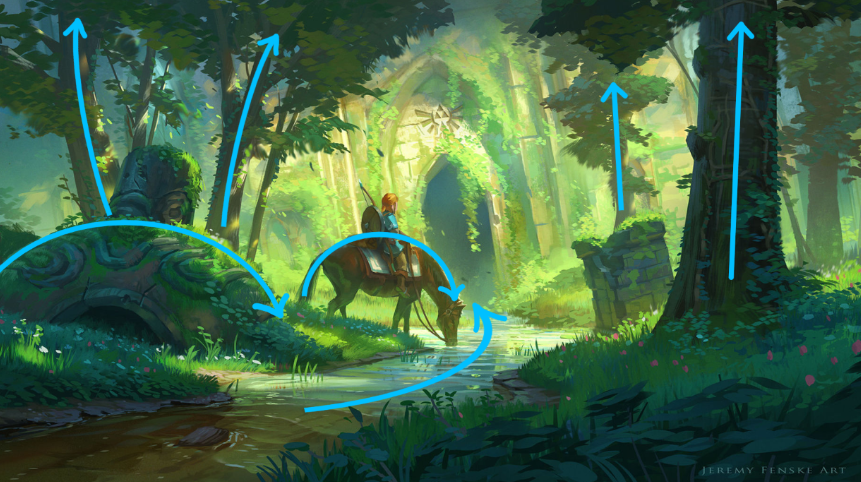
\includegraphics[width=\textwidth]{images/Saúl/Sección 3/EA_img3_2Composicion_3RutaVisual.png}
      \caption{\small 4.3.2.3 Ruta visual}
    \end{figure}

 En esta ilustración podemos apreciar como la principal ruta visual es el río que va desde abajo a la izquierda recorriendo toda la imagen hasta dentro del templo con la ayuda del personaje principal que trae la atención de la parte izquierda de la imagen, luego por otro lado están los árboles que son elementos importantes para el recorrido visual estos tiran la vista hacia el cielo intuyo que para dirigirte la mirada a donde hay luz y la luz te vuelva a dirigir dentro del templo, ya que el templo está iluminado con toda esta luz haciendo que gane mucha relevancia.

    \begin{figure}[H]
      \centering
      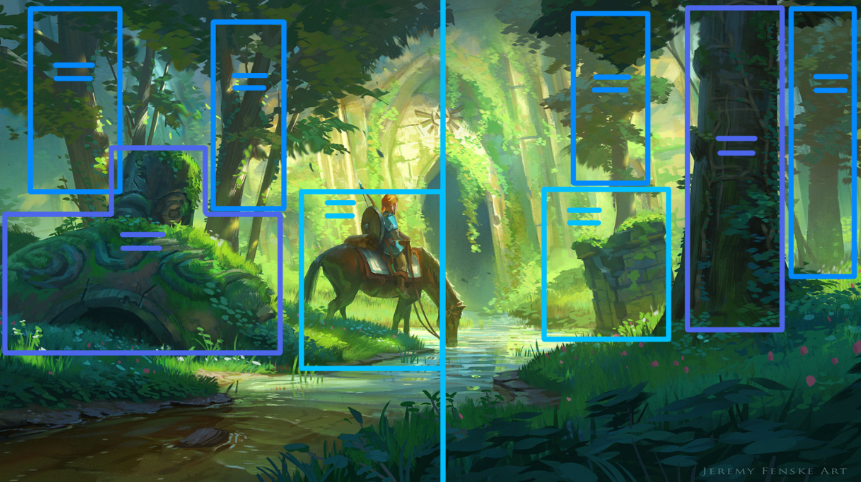
\includegraphics[width=\textwidth]{images/Saúl/Sección 3/EA_img3_2Composicion_4LeyBalanza-Simetria.png}
      \caption{\small 4.3.2.4 Ley de la balanza, equilibrio de pesos y simetría vs. asimetría}
    \end{figure}

Esta ilustración cumple con la ley de la balanza, ya que si partimos la imagen por la mitad más o menos los elementos que componen la imagen tienen el mismo peso, marcados con colores nos podemos fijar que están el personaje con el caballo y al otro lado la ruina de la columna en el azul-morado tenemos al árbol grande y haciéndole el contrapeso el guardián y por último tenemos a los 4 árboles del fondo que estos además de tener el mismo peso son simétricos. De hecho la imagen en sí guarda bastante simétrica solo hay que mirar la disposición de los colores están azul oscuro morado azul oscuro y azul claro y en el otro lado del eje de simetría están igual.



        \subsubsection{Claroscuro}

        
    \begin{figure}[H]
      \centering
      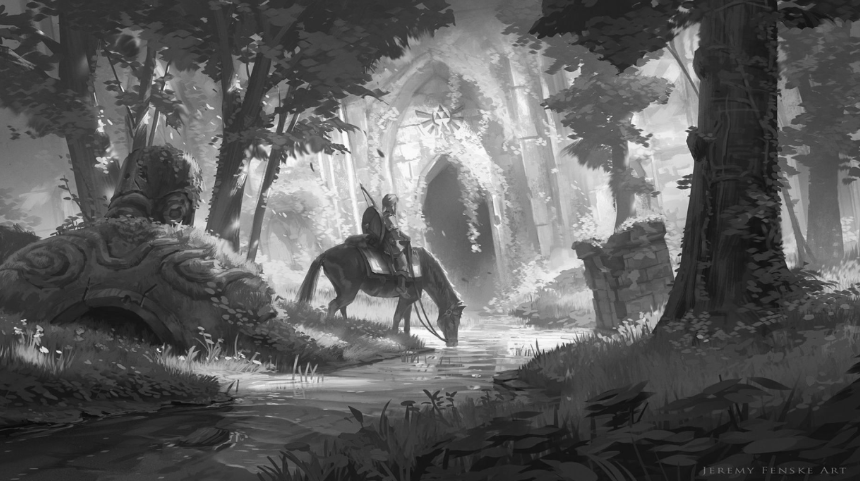
\includegraphics[width=\textwidth]{images/Saúl/Sección 3/EA_img3_3Claroscuro_1Profundidad.png}
      \caption{\small 4.3.3.1 Uso del claroscuro para representar la profundidad}
    \end{figure}

A nivel del claroscuro, podemos apreciar que las zonas más oscuras se sitúan en el primer plano y luego la zona de profundidad donde tenemos una clave alta es decir con más luminosidad esta se sitúa en la parte más lejana, lo que produce un contraste y crea esa sensación de profundidad en la imagen.

    \begin{figure}[H]
      \centering
      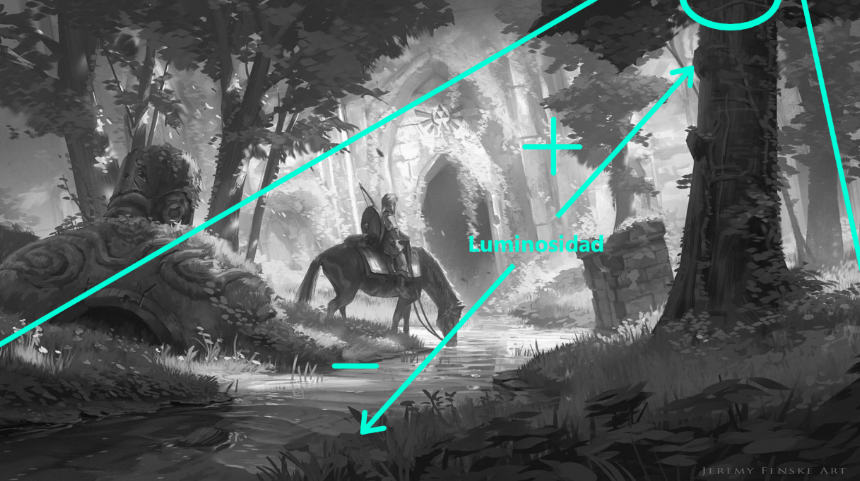
\includegraphics[width=\textwidth]{images/Saúl/Sección 3/EA_img3_3Claroscuro_2Luminosidad.png}
      \caption{\small 4.3.3.2 Zonas más luminosas y menos, y ubicación de la fuente de iluminación}
    \end{figure}

En esta imagen tenemos dos zonas, la zona de clave alta que sería la que está más al fondo con mucha luz y luminosidad y luego la zona de clave baja que se sitúa en el primer plano y la que está bañada con todas esas sombras. La ubicación de la fuente de luz, es la semicircunferencia que tenemos arriba a la derecha en dirección a la mayor luminosidad.

    \begin{figure}[H]
      \centering
      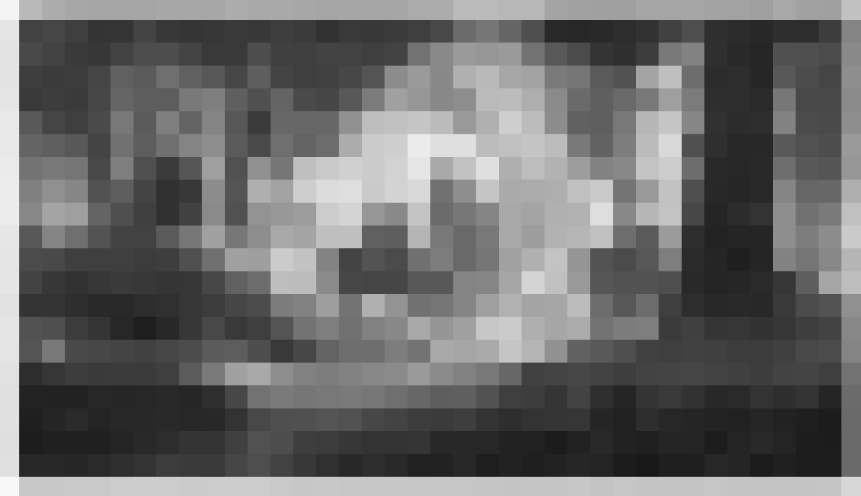
\includegraphics[width=\textwidth]{images/Saúl/Sección 3/EA_img3_3Claroscuro_3Clave.png}
      \caption{\small 4.3.3.3 Clave de la imagen}
    \end{figure}

Esta ilustración es una clave media, ya que aunque existen dos zonas bien diferenciadas como son el primer plano con una clave baja y la zona de profundidad con una clave alta, Al pixelar la imagen con los niveles de grises, podemos apreciar con mayor claridad que no hay ninguno que predomine sobre el otro hay más o menos la misma cantidad de claro que de oscuro, es por ello que la ilustración es una clave media.

        \subsubsection{Color}


    \begin{figure}[H]
      \centering
      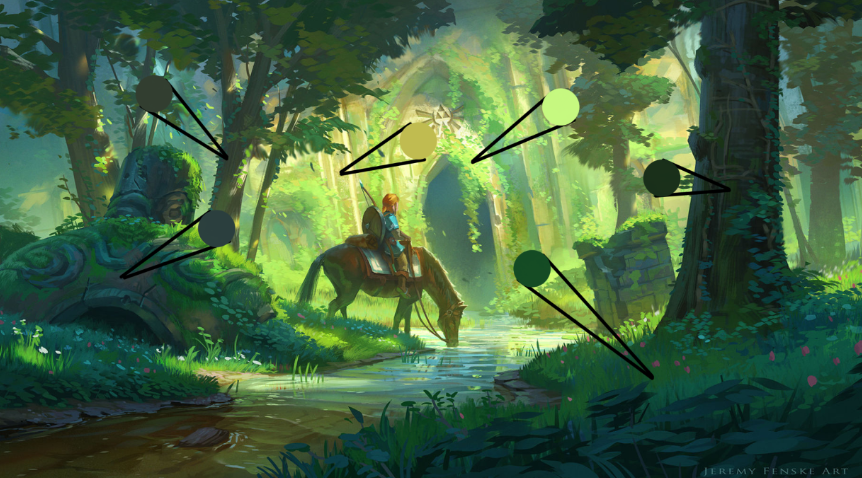
\includegraphics[width=\textwidth]{images/Saúl/Sección 3/EA_img3_4Color_1TonalidadGenral.png}
      \caption{\small 4.3.4.1 Tonalidad de color global}
    \end{figure}

La imagen tiene una tonalidad de color global fría, pero no es su totalidad, ya que está compuesta por las diferentes tonalidades de verdes (que sería la parte fría que envuelve toda la imagen) y los diferentes tonos de amarillos que destacan dada la excesiva luminosidad que reciben (está seria la parte cálida de la imagen). Hay un gran balance entre ambos colores, pero sin embargo predomina al ojo el verde porque es el color que mejor percibimos, por eso tiene una tonalidad fría.

    \begin{figure}[H]
      \centering
      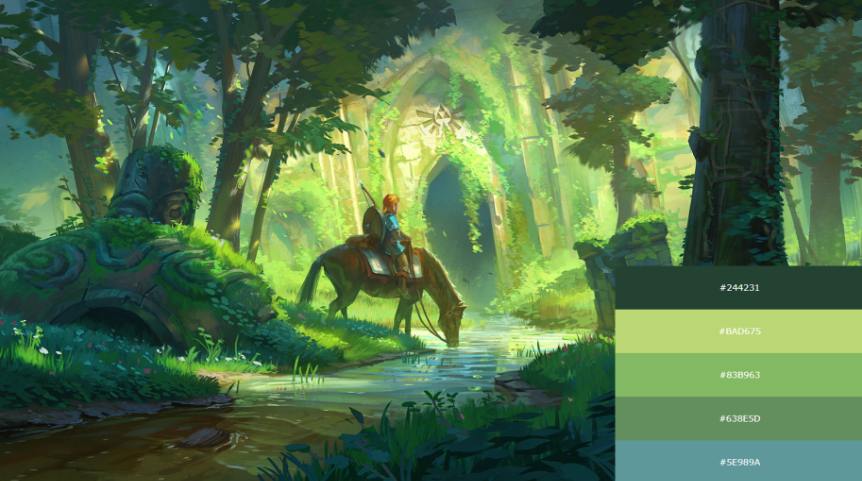
\includegraphics[width=\textwidth]{images/Saúl/Sección 3/EA_img3_4Color_2GamaColores.png}
      \caption{\small 4.3.4.2 Gama de color empleada}
    \end{figure}

La gama de colores empleada en esta imagen consta de una gama de tonalidades de verdes análogos entre ellos, incluso llegando a ampliar hasta algún amarillo en la fachada de las ruinas del templo del fondo. Sin embargo el cambio entre estos dos colores es muy suave, puesto que el verde es un color secundario procedente del amarillo.

    \begin{figure}[H]
      \centering
      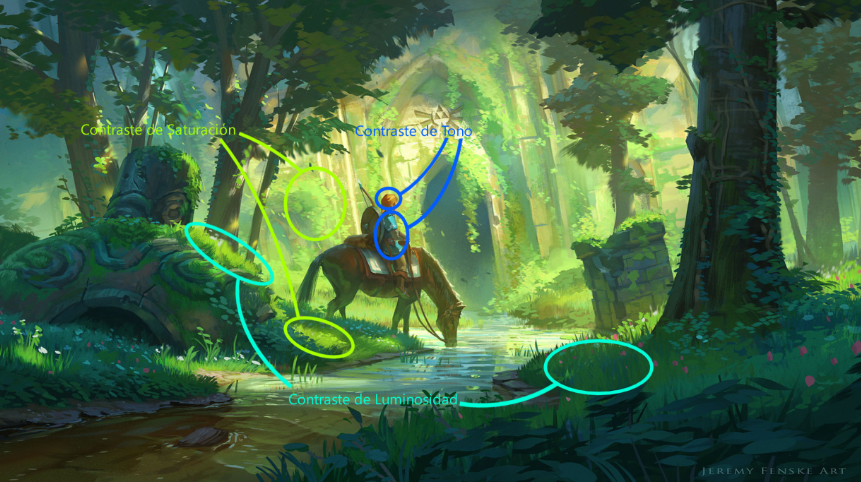
\includegraphics[width=\textwidth]{images/Saúl/Sección 3/EA_img3_4Color_3Contrastes.png}
      \caption{\small 4.3.4.3 Tipos de contraste}
    \end{figure}

En el contraste de saturación podemos encontrar una diferencia de intensidad del color entre dos o más elementos visuales en este caso en la imagen he marcado dos verdes uno más próximo a los primeros planos y el otro en el plano del fondo. El contraste de tono es la diferencia en el tono o matiz del color entre dos o más elementos visuales, esto se da entre colores cálidos y colores fríos, por ellos he marcado los colores complementarios del pelo del protagonista y la ropa del mismo. El contraste de luminosidad es la diferencia en el brillo o la luminosidad entre dos o más elementos visuales. Este se utiliza para destacar ciertos elementos o para crear una sensación de profundidad, por ello he marcado dos tonalidades de verde que están en distintos planos de profundidad uno al fondo y otro en el primer plano.

    \begin{figure}[H]
      \centering
      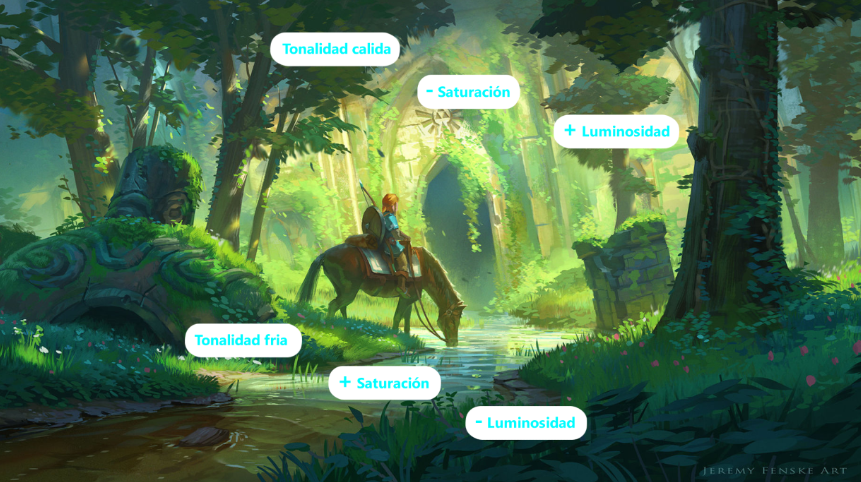
\includegraphics[width=\textwidth]{images/Saúl/Sección 3/EA_img3_4Color_4AnalisisPlanosPrimeroFondo.png}
      \caption{\small 4.3.4.4 Análisis de los colores empleados en primer y último plano}
    \end{figure}

En esta ilustración podemos ver como los colores utilizados en el primer plano están bastante más saturados que los se encuentran al fondo de la ilustración y pasa al contrario con la luminosidad que en el primer plano nos encontramos con colores con menos luminosidad y al fondo con más luminosidad. Por tanto esto nos deja con unos colores más claros y menos saturados en el último plano para crear una sensación de profundidad y hacer que los elementos del primer plano se destaquen o llamen la atención. Por otro lado pasa lo mismo con la tonalidad, se utilizan tonos fríos en el primer plano y tonos cálidos en el último plano para crear esa sensación de profundidad.
        \newpage

%-----------------------------------------------------------------
%-----------------------------------------------------------------

    \subsection{4. Raúl}
    
    \begin{figure}[H]
      \centering
      \includegraphics[width=\textwidth]{images/Concepts/4_concept_art}
      \caption{\small 4. Imagen}
\end{figure}

        \subsubsection{Perspectiva}
        
  \begin{figure}[H]
      \centering
      \includegraphics[width=\textwidth]{images/Raúl/Sección 4/Imagen 4 horizonte.jpg}
      \caption{\small 4. Horizonte}
\end{figure}       

La línea del horizonte podemos observar que se encuentra a una altura media, por lo tanto en este dibujo se podría decir que tenemos una vista serena.

\begin{figure}[H]
      \centering
      \includegraphics[width=\textwidth]{images/Raúl/Sección 4/Imagen 4 p. fuga.jpg}
      \caption{\small 4. Puntos de fuga}
\end{figure}  

Este dibujo presenta elementos orgánicos por los que no podemos saber con exactitud los puntos de fuga que aparecen en la imagen, sin embargo guiándonos por las formas de las montañas y algunos elementos de la imagen podríamos intuir que esta imagen tiene 1 único punto de fuga situado en el centro. Esto depende del punto de vista de cada persona, ya que como he dicho antes son elementos muy orgánicos y no se puede sacar nada con exactitud.

        \subsubsection{Composición}
        
\begin{figure}[H]
      \centering
      \includegraphics[width=\textwidth]{images/Raúl/Sección 4/Imagen 4 - 2 3.jpg}
      \caption{\small 4. Regla de los 2/3}
\end{figure}  

En esta imagen podemos observar como hay elementos a ambos lados, sin embargo el elemento principal, en este caso link encima del caballo, ocupa ligeramente el centro de esta regla de los 2/3.

\begin{figure}[H]
      \centering
      \includegraphics[width=\textwidth]{images/Raúl/Sección 4/Imagen 4 p. interes.jpg}
      \caption{\small 4. Puntos de interés}
\end{figure}  

Los puntos de interés principales son Link y su caballo el primero, ya que es el protagonista y siempre llama mucho la atención, después la montaña, ya que es un elemento muy grande y prácticamente el único en el fondo por lo que capta mucha atención y por último la escultura de piedra que se encuentra al lado izquierdo de Link, ya que es grande e inusual.

\begin{figure}[H]
      \centering
      \includegraphics[width=\textwidth]{images/Raúl/Sección 4/Imagen 4 recorrido visual.jpg}
      \caption{\small 4. Recorrido visual}
\end{figure}  

El recorrido visual de esta imagen se centra sobre todo en Link montado en su caballo, ya que está muy solitario en la imagen. Primeramente podemos guiarnos desde la escultura de la izquierda de la imagen la cual gracias a su forma y a su sombra nos guía hacia el protagonista del dibujo, el cual a su vez con la mirada y la posición de su caballo nos lleva a la montaña dividida en dos. Por otro lado también podemos empezar por la montaña la cual por su forma nos guía hacia link también, ya que es el elemento más importante. Otro camino de recorrido visual que se puede tomar son las montañas de la derecha, tanto la cercana como la del fondo, ya que tienen una forma como de tobogán lo que genera que llevemos la mirada de arriba hacia abajo y acabando de nuevo en Link.

\begin{figure}[H]
      \centering
      \includegraphics[width=\textwidth]{images/Raúl/Sección 4/Imagen 4 pesos.jpg}
      \caption{\small 4. Equilibrio y simetría}
\end{figure} 

        \subsubsection{Claroscuro}

\begin{figure}[H]
      \centering
      \includegraphics[width=\textwidth]{images/Raúl/Sección 4/Imagen 4 gris.jpg}
      \caption{\small 4. Claroscuro}
\end{figure} 

Poniendo la imagen en escala de grises podemos observar que las zonas más cercanas de la imagen son ligeramente más oscuras y las zonas más lejanas son de tonos más claros, no se nota mucho la diferencia, ya que es una imagen bastante luminosa, sin embargo se llega a apreciar ese cambio en la profundidad.

\begin{figure}[H]
      \centering
      \includegraphics[width=\textwidth]{images/Raúl/Sección 4/Imagen 4 gris luminosidad.jpg}
      \caption{\small 4. Luminosidad}
\end{figure}

La fuente de luz en esta imagen se encuentra en la esquina superior izquierda o por dicha zona. Podemos observar zonas como las del fondo que son más luminosas y las del primer plano más oscuras.

\begin{figure}[H]
      \centering
      \includegraphics[width=\textwidth]{images/Raúl/Sección 4/Imagen 4 gris pixel.jpg}
      \caption{\small 4. Pixelizada}
\end{figure}

Al pixelizar esta imagen podemos observar claramente que hay una dominancia de clave baja sobre todo por las nubes y el cielo y también por lo iluminada que está la mayoría de la imagen. Sin embargo podemos observar en las esquinas inferiores como aparecen ligeramente unos tonos más oscuros. En mi opinión es de clave alta, ya que domina los tonos claros.


        \subsubsection{Color}

\begin{figure}[H]
      \centering
      \includegraphics[width=\textwidth]{images/Raúl/Sección 4/Imagen 4 tonalidades.jpg}
      \caption{\small 4. Tonos de color}
\end{figure}
En esta imagen podemos observar un gran número de colores distintos sin embargo los que más dominan la imagen son los colores frios, ya que la mayoria de la imagen contiene distintas tonalidades de verdes. También podemos apreciar tonos de rojo en las flores de primer plano así como colores anaranjados en las montañas e incluso plateados en el escudo de Link. No obstante dominan los colores fríos.

\begin{figure}[H]
      \centering
      \includegraphics[width=\textwidth]{images/Raúl/Sección 4/Imagen 4 colores.jpg}
      \caption{\small 4. Gama de color}
\end{figure}

La gama de colores utilizada en esta imagen yo creo que es una triada de colores a su vez que en cada uno de los colores escogidos en la triada, tienen colores análogos, como por ejemplo el azul y el verde o los tonos anaranjados o los toques rojizos y rosados.

\begin{figure}[H]
      \centering
      \includegraphics[width=\textwidth]{images/Raúl/Sección 4/Imagen 4 contrastes.jpg}
      \caption{\small 4. Contrastes}
\end{figure}

En el contraste de luminosidad se puede observar de un mismo color distintos tonos, uno más claro y otro más oscuro para mostrar profundidad. Por otra parte tenemos el contraste de tono que encontramos en Link, ya que su ropa es de un color frío sin embargo su pelo es de un color cálido. Por último observamos un contraste de saturación en los diferentes tonos de verde del fondo y más cercanos, ya que tienen intensidades distintas.

\begin{figure}[H]
      \centering
      \includegraphics[width=\textwidth]{images/Raúl/Sección 4/Imagen 4 capas.jpg}
      \caption{\small 4. Capas}
\end{figure}

 En el primer plano podemos observar unas tonalidades más cálidas por las flores rojas, el camino y el caballo de link. En el segundo plano encontramos tonalidades más frías sobre todo por el cielo y las nubes. También podemos observar una diferencia en la luminosidad para generar efecto de profundidad y por último un mayor contraste de tonos por las flores y la tierra y una mayor saturación en los colores del fondo de la imagen.


        \newpage

%-----------------------------------------------------------------
%-----------------------------------------------------------------

    \subsection{5. Miquel}
        \begin{figure}[H]
      \centering
      \includegraphics[width=\textwidth]{images/Miquel/sección5/5_concept_art.png}
      \caption{\small 5. Imagen del juego}
    \end{figure}

    Se trata de una imagen oficial el juego, en el que podemos apreciar al protagonista inclinado mientras esta en unas islas flotantes

        \subsubsection{Perspectiva}

    \begin{figure}[H]
      \centering
      \includegraphics[width=\textwidth]{images/Miquel/sección5/vista1.png}
      \caption{\small 5. Línea del horizonte}
    \end{figure}

    La línea de horizonte se halla en medio de la imagen, esto es sabido por la posición de Link y de la isla a la que está el mismo situado, por lo tanto, podemos discernir que se trata de una vista de rana.


    \begin{figure}[H]
      \centering
      \includegraphics[width=\textwidth]{images/Miquel/sección5/puntosdefuga1.png}
      \caption{\small 5. puntos de fuga}
    \end{figure}

    Al saber que nos hallamos ante una imagen con una vista serena, podemos encontrar dos puntos de fuga, esto es sabido también por las construcciones  de las islas. Un punto de fuga se halla en la izquierda y el otro a la derecha.


        \subsubsection{Composición}
    \begin{figure}[H]
      \centering
      \includegraphics[width=\textwidth]{images/Miquel/sección5/1regla23png.png}
      \caption{\small 5. Regla 2/3}
    \end{figure}
    
    La regla de las 2/3 nos permite discernir que en los lados inferiores y centrales de la imagen es donde podemos hallar a los componentes que conforman la imagen, mientras que el lado superior se halla completamente libre, permitiendo respirar así a la imagen.

    \begin{figure}[H]
      \centering
      \includegraphics[width=\textwidth]{images/Miquel/sección5/puntosinteres1.png}
      \caption{\small 5. puntos de interes}
    \end{figure}

    Los puntos de interés que podemos encontrar en la imagen son, obviamente, Link, la isla en la que él está situado y por último las islas situadas a la izquierda, las cuales se hallan en el último plano.

    \begin{figure}[H]
      \centering
      \includegraphics[width=\textwidth]{images/Miquel/sección5/flechas1.png}
      \caption{\small 5. recorrido visual}
    \end{figure}

     El recorrido visual que se aprecia es que lleva a la fuente de luz de la imagen, la vista de Link, la esquina de la isla y el viento es una prueba de ello.

    \begin{figure}[H]
      \centering
      \includegraphics[width=\textwidth]{images/Miquel/sección5/leydelabalanza1.png}
      \caption{\small 5. Regla de la balanza}
    \end{figure}

    La ley de la balanza nos permite saber que el peso de la imagen está inclinada hacia la derecha, puesto que en la izquierda solo hay islas las cuales se hallan en el último plano.

        \subsubsection{Claroscuro}

    \begin{figure}[H]
      \centering
      \includegraphics[width=\textwidth]{images/Miquel/sección5/imagen-claroscuro.png}
      \caption{\small 5. Escala de grises}
    \end{figure}

    Al aplicar la escala de grises, podemos observar que el primer plano es donde se halla la parte oscura de la imagen, mientras más nos alejamos más clara se hacen los componentes de esta.

    \begin{figure}[H]
      \centering
      \includegraphics[width=\textwidth]{images/Miquel/sección5/imagen-luminosidad.png}
      \caption{\small 5. Luminosidad}
    \end{figure}

    En este caso, podemos observar que la fuente de luz se halla en la parte izquierda-centro, iluminando toda la imagen, exceptuando la sombra que proyecta Link y la parte de la isla que no está a la vista de la luz. Por tanto, la mayoría de la sombra la hallamos en la parte inferior izquierda.
    
   \begin{figure}[H]
      \centering
      \includegraphics[width=\textwidth]{images/Miquel/sección5/imagen-clave.png}
      \caption{\small 5. Clave}
    \end{figure}

Como resultado de lo anteriormente dicho, podemos decir que esta imagen es de clave alta, ya que presenta mucha iluminación.

        \subsubsection{Color}

 \begin{figure}[H]
      \centering
      \includegraphics[width=\textwidth]{images/Miquel/sección5/imagen-colores.png}
      \caption{\small 5. paleta de color}
    \end{figure}

     La tonalidad global de la imagen es fría, ya que está muy presente el color azul, aun a pesar de que podemos encontrar un amarillo saturado en el primer plano.  

\begin{figure}[H]
      \centering
      \includegraphics[width=\textwidth]{images/Miquel/sección5/imagen-gamas.png}
      \caption{\small 5. Gamas implementadas}
    \end{figure}

    La imagen presenta una serie de azules análogos en casi toda ella, aunque se halla tambien una serie de amarillos y verdes analogos en la vegetación de las islas.

\begin{figure}[H]
      \centering
      \includegraphics[width=\textwidth]{images/Miquel/sección5/imagen-contrastes.png}
      \caption{\small 5. tipos de contrastes}
    \end{figure}
    
    Podemos hallar una serie de contrastes en esta imagen. Primero, la diferencia de luminosidad que hay en la parte central de la imagen con la parte inferior izquierda, la diferencia de saturación entre  la isla del primer plano con las del último plano y la diferencia de tonos que hay entre la ropa de Link, que es de tonalidad fría, con la vegetación de la isla, que es de tonalidad cálida.

    \begin{figure}[H]
      \centering
      \includegraphics[width=\textwidth]{images/Miquel/sección5/imagen-colorfinal.png}
      \caption{\small 5. Analisis de la ultima y primera capa}
    \end{figure}

    En comparación entre el primer plano y el último, podemos observar que el primero presenta mayor saturación, menor luminosidad y es de tonalidad cálida, aunque no mucho, mientras que el último plano presenta menor saturación, mayor luminosidad y es de tonalidad fría.

%-----------------------------------------------------------------
%-----------------------------------------------------------------

    \subsection{6. Nerea (segunda imagen)}
    \begin{figure}[H]
      \centering
      \includegraphics[width=\textwidth]{images/Nerea/6_concept_art.png}
      \caption{\small 4.6.1 Imagen}
    \end{figure}
    Imagen compuesta por Link mirando hacía el imnenso castillo en la lejanía.

    
        \subsubsection{Análisis de la perspectiva}


    \begin{figure}[H]
      \centering
      \includegraphics[width=\textwidth]{images/Nerea/Nerea Zelda concept 611.PNG}
      \caption{\small 4.6.1.1 Línea del horizonte y tipo de vista}
    \end{figure}

    Gracias a el pie de la montaña que se encuentra al fondo a la izquierda, los evidentes y numerosos puntos de fuga presentes y las botas de Link orientados hacía arriba desde esa misma posición, se nos incita a pensar que la mirada y línea de horizonte se fija a la misma altura. La línea de horizonte expuesta en la parte inferior de la imagen indica que el tipo de vista es de rana. 
    Gracias a esto y al pequeño tamaño de nuestro héroe, se consigue acentuar todavía más la gran presencia y magnitud del castillo del fondo.

    \begin{figure}[H]
      \centering
      \includegraphics[width=\textwidth]{images/Nerea/Nerea Zelda concept 621.PNG}
      \caption{\small 4.6.1.2 Puntos de fuga}
    \end{figure}

    Supondré que la ilustración tiene 6 puntos de fuga, gracias al castillo en la lejanía podemos ver cómo las diferentes paredes, suelo y torres del mismo fugan, excepto el del medio y el situado detrás de las rocas a la derecha, hacía puntos situados fuera de la imagen. Este apartado no se puede saber a ciencia cierta debido a que la gran estructura que se encuentra en el fondo, al tener numerosas paredes inclinadas o en mal estado, entorpece una correcta interpretación de todos los puntos de fuga al completo.

        \subsubsection{Análisis de la composición}

        
    \begin{figure}[H]
      \centering
      \includegraphics[width=\textwidth]{images/Nerea/Nerea Zelda concept 621.PNG}
      \caption{\small 4.6.2.1 Regla de los 2/3}
    \end{figure}

    La ilustración presenta un castillo que ocupa todo el centro superior. Las rocas gigantes llenan prácticamente toda la sección vertical derecha y el héroe representado en pequeño en la esquina inferior izquierda. Podemos observar también como la imagen respira por la parte central inferior y por la parte superior izquierda, cuya notable luminosidad y vasta profundidad permite posar y relajar la mirada después de haber visto los demás elementos o puntos de interés o antes de lanzarse a ello.

    \begin{figure}[H]
      \centering
      \includegraphics[width=\textwidth]{images/Nerea/Nerea Zelda concept 622.PNG}
      \caption{\small 4.6.2.2 Puntos de interés, principal y secundarios}
    \end{figure}

    La ilustración presenta un castillo como principal de centro atracción visual, seguido de unas grandes rocas en la parte derecha que, aunque parezcan solo apoyos visuales, su inmensa dimensión y cercanía hace que forme parte, junto con Link, de los puntos de interés secundarios. El punto de interés principal será el monumental castillo, mientras que los puntos de interés secundarios serán las rocas y nuestro héroe.

    \begin{figure}[H]
      \centering
      \includegraphics[width=\textwidth]{images/Nerea/Nerea Zelda concept 623.PNG}
      \caption{\small 4.6.2.3 Recorrido visual}
    \end{figure}

    La ruta podría comenzar tanto en Link y las rocas en las que se alza, la incidente luz celestial o las puntiagudos extremos de las rocas. Si comienza en Link y/o rocas, estas últimas y la atención del personaje dirigirá el recorrido hacia la colina que sube cuesta arriba hacia el castillo. Por otro lado, tenemos una incidente luz proyectada sobre gran parte de la ilustración hacía abajo y la derecha cuyos rayos también consiguen dirigir nuestra mirada en dirección al punto de interés principal, el deteriorado castillo.

    \begin{figure}[H]
      \centering
      \includegraphics[width=\textwidth]{images/Nerea/Nerea Zelda concept 624.PNG}
      \caption{\small 4.6.2.4 Ley de la balanza, equilibrio de pesos y simetría vs. asimetría}
    \end{figure}

    La imagen cumple la ley de la balanza ya que, a pesar del evidente peso recae sobre la parte derecha, la luminosidad y una parte mayor del castillo en la parte izquierda pesan lo suficiente como para contrarrestar a los elementos de la derecha y su poca luminosidad. Por consiguiente, la imagen es simétrica al no presentar ningún desequilibrio final.


        \subsubsection{Claroscuro}

        
    \begin{figure}[H]
      \centering
      \includegraphics[width=\textwidth]{images/Nerea/Nerea Zelda concept 631.PNG}
      \caption{\small 4.6.3.1 Uso del claroscuro para representar la profundidad}
    \end{figure}

    Gracias al filtro en blanco y negro utilizado en la ilustración, es fácil ver como la profundidad es representada. Tenemos las zonas más cercanas muy oscuras situadas desde la parte central abajo hasta la parte derecha central y superior, poco a poco alejándose hacia el distante castillo. Luego, por otro lado tenemos unas zonas más alejadas muy iluminadas encontradas a la izquierda de la imagen, que justo coincide también con el plano secundario o fondo de la imagen. Este contraste nos hace ver que la profundidad aumenta conforme la mirada se aleja de la zona central inferior hacia la derecha y derecha superior, hasta por fin llegar al fondo situado en el extremo izquierdo superior y central.

    \begin{figure}[H]
      \centering
      \includegraphics[width=\textwidth]{images/Nerea/Nerea Zelda concept 632.PNG}
      \caption{\small 4.6.3.2 Zonas más luminosas y menos, y ubicación de la fuente de iluminación}
    \end{figure}

    La fuente de luz, al encontrarse en detrás de un cielo nublado en una parte de la esquina superior izquierda, genera unas zonas más luminosas en a la izquierda por proximidad mientras que una clara ausencia de luz será visible en la parte derecha, la cúal será menos iluminada. Debido a esta ubicación de la fuente de iluminación y la distribución escogida para las montañas y senderos, vemos como la luminosidad va de mayor luminancia desde la izquierda hasta el centro, pero los rayos de luz no llegan a alcanzar el resto de la ilustración a la derecha.

    \begin{figure}[H]
      \centering
      \includegraphics[width=\textwidth]{images/Nerea/Nerea Zelda concept 633.PNG}
      \caption{\small 4.6.3.3 Clave de la imagen}
    \end{figure}

    Nos encontramos ante una clave media. Aunque la clave alta de la izquierda y la clave baja de la derecha alcanzan gran notoriedad, debido a que la mayor parte de la ilustración presenta una clave media y encima esta está situada en la parte central, todavía le da más importancia y resalta esa mayoría.


        \subsubsection{Color}


    \begin{figure}[H]
      \centering
      \includegraphics[width=\textwidth]{images/Nerea/Nerea Zelda concept 641.PNG}
      \caption{\small 4.6.4.1 Tonalidad de color global}
    \end{figure}

    La ilustración tiene una clara tonalidad de color global fría. Si bien es verdad que se pueden percibir numerosos tonos cálidos por la parte del centro hacía abajo y gran parte de la izquierda (rayos sol amarillentos y la verde colina más los cálidos ropajes y pelo de Link), no son suficientes para eclipsar la inmensa presencia de los tonos fríos.

    \begin{figure}[H]
      \centering
      \includegraphics[width=\textwidth]{images/Nerea/Nerea Zelda concept 642.PNG}
      \caption{\small 4.6.4.2 Gama de color empleada}
    \end{figure}

    La gama de colores empleada en esta ilustración incluye una gama de tonalidades de naranjas/amarillas análogas, seguida de otra gama de tonalidades de verdes análogos que ya se va juntando y relaciona con los tonos fríos señalados en la parte superior derecha. La gama más utilizada y amplia es sin duda la de tonalidades azules análogas.

    \begin{figure}[H]
      \centering
      \includegraphics[width=\textwidth]{images/Nerea/Nerea Zelda concept 643.PNG}
      \caption{\small 4.6.4.3 Tipos de contraste}
    \end{figure}

    En el contraste de saturación es posible discernir cambios en la intensidad de unos colores a otros, como por ejemplo el mostrado a la izquierda del todo, que son dos tonos azules prácticamente iguales que se encuentran saturados de diferente forma ya que las partes más cercanas deben estar más saturadas mientras las más alejadas deben estarlo mucho menos para conseguir profundidad. El contraste de tono está presente cuando, entre dos o más elementos visuales, es posible encontrar distinciones en cuanto a tono o matiz de sus respectivos colores. Esto ocurre entre colores cálidos y colores fríos, he señalado los colores complementarios del pelo del protagonista y las nubes cercanas a él. El contraste de luminosidad es la diferencia de luminosidad entre dos o más elementos visuales. Empleado para resaltar ciertos elementos variando la cantidad de luz/sombra aplicada o para conseguir un efecto de profundidad, En este caso he señalado dos tonalidades azules cuya luminosidad cambia en función del foco de luz y ayuda a representar las sombras proyectadas por este.

    \begin{figure}[H]
      \centering
      \includegraphics[width=\textwidth]{images/Nerea/Nerea Zelda concept 644.PNG}
      \caption{\small 4.6.4.4 Análisis de los colores empleados en primer y último plano}
    \end{figure}

    Es posible apreciar cómo los colores escogidos para el primer plano están muy saturados en comparación con los del fondo mientras que, a la hora de tener en cuenta la luminancia, el último plano tiene colores con mucha más luminosidad que los del primer plano. En cuanto a la tonalidad, con el fin de representar la profundidad, se usan tonos cálidos en el primer plano y fríos en el último.
        \newpage

%-----------------------------------------------------------------
%-----------------------------------------------------------------

    \subsection{7. Miquel (segunda imagen)}
    \begin{figure}[H]
      \centering
      \includegraphics[width=\textwidth]{images/Miquel/sección7/7_concept_art.jpg}
      \caption{\small 7. fan art}
    \end{figure}

    Se trata de un fan art, en el podemos apreciar a un guardián y el castillo de Hyrule.

        \subsubsection{Perspectiva}

    \begin{figure}[H]
      \centering
      \includegraphics[width=\textwidth]{images/Miquel/sección7/vista2.png}
      \caption{\small 7. Línea de horizonte}
    \end{figure}

    La línea de horizonte se halla en la parte inferior de la imagen, esto es sabido por el límite del terreno. Podemos discernir que es una vista de rana debido a la posición de la línea y de los componentes de la imagen.
    
    \begin{figure}[H]
      \centering
      \includegraphics[width=\textwidth]{images/Miquel/sección7/puntosdefuga2.png}
      \caption{\small 7. puntos de fuga}
    \end{figure}

    Al saber que nos hallamos ante una imagen con una vista rana, podemos suponer que hay tres puntos de fuga, aunque solo ha sido posible encontrar uno debido a la insuficiencia de componentes que nos puedan indicar donde se hallan los otros dos puntos.

        \subsubsection{Composición}
    \begin{figure}[H]
      \centering
      \includegraphics[width=\textwidth]{images/Miquel/sección7/2regla23.png}
      \caption{\small 7. Regla 2/3}
    \end{figure}
    
    La regla de las 2/3 nos permite discernir que el lado izquierdo y centro es donde más se hallan los componentes de la imagen, siendo la parte superior derecha la que permite respirar a la imagen.

    \begin{figure}[H]
      \centering
      \includegraphics[width=\textwidth]{images/Miquel/sección7/puntosdeinteres2.png}
      \caption{\small 7. puntos de interes}
    \end{figure}

    Los puntos de interés que podemos encontrar en la imagen son, el guardián del primer plano, el aura morada que nos conduce al castillo y a las estructuras cercanas al castillo.

    \begin{figure}[H]
      \centering
      \includegraphics[width=\textwidth]{images/Miquel/sección7/flechas2.png}
      \caption{\small 7. recorrido visual}
    \end{figure}

    El recorrido visual nos permite saber que todo conduce al castillo: el camino en el lado derecho, el aura morada  que nos conduce a unas estructuras, las cuales apuntan al castillo y la forma de las nubes.

    \begin{figure}[H]
      \centering
      \includegraphics[width=\textwidth]{images/Miquel/sección7/leydelabalanza2.png}
      \caption{\small 7. Regla de la balanza}
    \end{figure}

    La ley de la balanza nos permite discernir que en el lado izquierdo se encuentra el guardián, en el medio de la balanza se halla el castillo y el lado derecho las estructuras y vegetación, brindando así a la imagen cierto equilibrio
   
        \subsubsection{Claroscuro}

    \begin{figure}[H]
      \centering
      \includegraphics[width=\textwidth]{images/Miquel/sección7/imagen2-claroscuro.png}
      \caption{\small 7. Escala de grises}
    \end{figure}
    
    Al aplicar la escala de grises, podemos observar que el primer plano es donde se halla la parte más oscura de la imagen, mientras más nos alejamos más clara se hacen los componentes de esta.

    \begin{figure}[H]
      \centering
      \includegraphics[width=\textwidth]{images//Miquel/sección7/imagen2-luminosidad.png}
      \caption{\small 7. Luminosidad}
    \end{figure}

    En este caso, podemos observar que la fuente de luz se halla en la parte derecha centro, siendo esta tapada por las nubes y la montaña.
    
    \begin{figure}[H]
      \centering
      \includegraphics[width=\textwidth]{images//Miquel/sección7/imagen2-clave.png}
      \caption{\small 7. Clave}
    \end{figure}

    Como resultado de lo anteriormente dicho, podemos decir que esta imagen es de clave media , ya que presenta mucha iluminación en el fondo y se va oscureciendo conforme se acerca.

        \subsubsection{Color}
\begin{figure}[H]
      \centering
      \includegraphics[width=\textwidth]{images//Miquel/sección7/imagen2-colores.png}
      \caption{\small 7. paleta de color}
    \end{figure}

     La tonalidad global de la imagen es fría, ya que está muy presente el color azul y verde.   

\begin{figure}[H]
      \centering
      \includegraphics[width=\textwidth]{images//Miquel/sección7/imagen2-gamas.png}
      \caption{\small 7. Gamas implementadas}
    \end{figure}
  
    La imagen presenta una serie de azules análogos en el cielo y fondo, unos morados análogos en un componente de la imagen y una serie de verdes análogos en el terreno.

\begin{figure}[H]
      \centering
      \includegraphics[width=\textwidth]{images//Miquel/sección7/imagen2-contrastes.png}
      \caption{\small 7. tipos de contrastes}
    \end{figure}
    
    Podemos hallar una serie de contrastes en esta imagen. Primero, la diferencia de luminosidad que hay en la parte derecha inferior de la imagen con la parte inferior izquierda, la diferencia de saturación entre la flor azul del primer plano con el azul del cielo  y la diferencia de tonos que hay entre el verde saturado del terreno con el morado del aura.

    \begin{figure}[H]
      \centering
      \includegraphics[width=\textwidth]{images//Miquel/sección7/imagen2-final.png}
      \caption{\small 7. Analisis de la última y primera capa}

    En comparación entre el primer plano y el último, podemos observar que el primero presenta mayor saturación, menor luminosidad y es de tonalidad fría, mientras que el último plano presenta menor saturación, mayor luminosidad y es de tonalidad fría, igual que el primero.


    \end{figure}
%-----------------------------------------------------------------
%-----------------------------------------------------------------

    \subsection{8. Raúl (Segunda imagen)}
    \begin{figure}[H]
      \centering
      \includegraphics[width=\textwidth]{images/Concepts/8_concept_art}
      \caption{\small 8. Imagen}
    \end{figure}

        \subsubsection{Perspectiva}

\begin{figure}[H]
      \centering
      \includegraphics[width=\textwidth]{images/Raúl/Sección 8/Imagen 8 horizonte.jpg}
      \caption{\small 8. Línea de horizonte}
    \end{figure}

La línea de horizonte se puede intuir que está en la zona de abajo y por ello se puede decir también que es vista de rana.

\begin{figure}[H]
      \centering
      \includegraphics[width=\textwidth]{images/Concepts/8_concept_art}
      \caption{\small 8. Puntos de fuga}
    \end{figure}
    
En esta imagen no podemos saber con certeza los puntos de fuga, ya que es una imagen con elementos orgánicos, aun así podemos intuir que es una imagen con 3 puntos de fuga, ya que si seguimos las líneas de la luz proporcionada de la luna podemos observar que todas fugan hacia un mismo punto y por la vista de rana sabemos que existe la posibilidad de que tenga 3 puntos de fuga, sin embargo esto no podemos saberlo seguros, ya que como he dicho antes es una imagen orgánica y no proporciona a penas información sobre los puntos de fuga.

        \subsubsection{Composición}

\begin{figure}[H]
      \centering
      \includegraphics[width=\textwidth]{images/Raúl/Sección 8/Imagen 8 2 3.jpg}
      \caption{\small 8. Regla de los 2/3}
    \end{figure}

En esta imagen se ve claramente como la imagen está completamente centrada, ya que ocupa los tercios centrales con la mayoría de elementos importantes de la imagen.

\begin{figure}[H]
      \centering
      \includegraphics[width=\textwidth]{images/Raúl/Sección 8/Imagen 8 p. interes.jpg}
      \caption{\small 8. Puntos de interés}
    \end{figure}

Los diferentes puntos de interés que podemos encontrar en la imagen son principalmente el monstruo gigante y a su vez la luna que tiene en la espalda, después a Link, ya que por su ropa hace un contraste que genera que sea un punto de interés principal y por último tenemos la espada de link que está brillando por la luz de la luna y eso llama la atención y la espada del monstruo que al ser muy grande también genera cierto interés.

\begin{figure}[H]
      \centering
      \includegraphics[width=\textwidth]{images/Raúl/Sección 8/Imagen 8 recorridos.jpg}
      \caption{\small 8. Recorrido visual}
    \end{figure}

Podemos observar como todo nos guía hacia la luna o en su defecto hacia el monstruo que está justo en frente de esta. Uno de los primeros recorridos visuales que encontramos es por el arma del monstruo hacia su brazo y finalmente a su cabeza. Si tomamos otro camino como por ejemplo el césped de una de las esquinas inferiores de la imagen, ambos recorridos nos guían a Link, por la posición de su cuerpo y su mirada nos guía hacia la cara del enemigo. Por otra parte podemos tomar el camino de la espada que hace el mismo que el del césped o el de las nubes que nos guían todas hacia la cabeza del monstruo.

\begin{figure}[H]
      \centering
      \includegraphics[width=\textwidth]{images/Raúl/Sección 8/Imagen 8 regla pesos.jpg}
      \caption{\small 8. Equilibrio y simetría}
    \end{figure}

En esta imagen a simple vista podemos pensar que esta imagen no está equilibrada, ya que el arma del monstruo ejerce mucho más peso en el dibujo que la espada de Link. Sin embargo si nos fijamos bien hay un árbol que contrarresta el peso del arma del monstruo en gran aparte y logra que la imagen esté equilibrada, ya que a un lado tenemos la mitad del monstruo y su arma y al otro tenemos la otra mitad del monstruo, Link con su espada y finalmente el árbol por lo que podríamos concluir con que está equilibrada la imagen. 


        \subsubsection{Clarooscuro}

\begin{figure}[H]
      \centering
      \includegraphics[width=\textwidth]{images/Raúl/Sección 8/Imagen 8 gris.jpg}
      \caption{\small 8. Claroscuro}
    \end{figure}

 Pasando la imagen a escala de grises podemos observar como las zonas más cercanas, en este caso link y el monstruo son más oscuras que las lejanas como son los árboles y la maleza. Esto genera un efecto de profundidad en la foto.

\begin{figure}[H]
      \centering
      \includegraphics[width=\textwidth]{images/Raúl/Sección 8/Imagen 8 gris lumin.jpg}
      \caption{\small 8. Luminosidad}
    \end{figure}

 En esta imagen se ve claramente que el foco de luz es la luna, por lo tanto es la zona con más luminosidad y conforme más nos acercamos al protagonista menos luminosidad hay. Sin embargo en la espada de Link hay un reflejo que le da mucha luminosidad y hace un contraste entre las sombras del monstruo y Link y este brillo.

\begin{figure}[H]
      \centering
      \includegraphics[width=\textwidth]{images/Raúl/Sección 8/Imagen 8 gris pixel.jpg}
      \caption{\small 8. Pixel}
    \end{figure}

 En esta imagen podemos observar que pese a ser de noche hay una clave media, ya que la luna ofrece una luminosidad que genera tonos más claros y además con su propio brillo hace que no domine tanto el gris oscuro, por lo que en mi opinión esta imagen es de clave media.

        \subsubsection{Color}

\begin{figure}[H]
      \centering
      \includegraphics[width=\textwidth]{images/Raúl/Sección 8/Imagen 8 tonos.jpg}
      \caption{\small 8. Tonos de color}
    \end{figure}

En esta imagen al ser de noche podemos observar una dominancia de los tonos fríos, sin embargo el pelaje del monstruo y el pelo de Link genera un contraste, ya que son colores más cálidos.

\begin{figure}[H]
      \centering
      \includegraphics[width=\textwidth]{images/Raúl/Sección 8/Imagen 8 colores.jpg}
      \caption{\small 8. Gama de color}
    \end{figure}

 La gama de colores utilizada en esta imagen son colores compuestos, ya que se usan 4 colores complementarios 2 a 2 con sus respectivas tonalidades.

\begin{figure}[H]
      \centering
      \includegraphics[width=\textwidth]{images/Raúl/Sección 8/Imagen 8 contraste.jpg}
      \caption{\small 8. Contraste}
    \end{figure}

Podemos observar un contraste de luminosidad por ejemplo en el pelaje del monstruo, ya que tiene una zona más oscura por delante y por el lado se ve como le da la luz de la luna y esto genera que haya colores más luminosos. Por otro lado tenemos un contraste de tono entre la ropa de Link y el pelaje del monstruo, ya que el ropaje de Link es de un tono frío y el pelaje de uno cálido. Por último un contraste de saturación en el cielo, ya que cuanto más lejos está el cielo más saturado se observa.

\begin{figure}[H]
      \centering
      \includegraphics[width=\textwidth]{images/Raúl/Sección 8/Imagen 8 capas.jpg}
      \caption{\small 8. Capas}
    \end{figure}

En esta imagen se pueden observar diferencias por ejemplo en la tonalidad, ya quee en el primer plano tenemos tonos cálidos por el monstruo y en el fondo tonos fríos por el cielo y la luna. También tenemos una diferencia en la saturación, ya que cuanto más alejada la imagen más saturada se ve. Por último una diferencia muy notoria en la luminosidad, ya que cuanto más cerca el elemento, por ejemplo el monstruo, más oscuro se ve y cuánto más lejos, por ejemplo las nubes más luminoso.

        \newpage

%-----------------------------------------------------------------
%-----------------------------------------------------------------

    \subsection{9. Alonso}
    \begin{figure}[H]
      \centering
      \includegraphics[width=\textwidth]{images/Concepts/9_concept_art}
      \caption{\small 9. Imagen}
    \end{figure}
    Se trata de una imagen oficial del juego, la portada del mismo.

        \subsubsection{Perspectiva}

    \begin{figure}[H]
      \centering
      \includegraphics[width=\textwidth]{images/Alonso/Sección 9/Linea orizonte}
      \caption{\small 9. Línea del horizonte}
    \end{figure}

    Comenzaremos hablando de la línea del horizonte la cual está situada justo en medio de la imagen. Se puede discernir perfectamente debido a que se encuentra directamente el propio horizonte en la lejanía delimitado por una línea perfectamente recta. En función de estos datos podemos concluir  que se trata de una vista serena.

    \begin{figure}[H]
      \centering
      \includegraphics[width=\textwidth]{images/Alonso/Sección 9/caja.jpg}
      \caption{\small 9. puntos de fuga}
    \end{figure}

    Cómo está estructurada la imagen no podremos sacar información de la misma. Los elementos son demasiado orgánicos como para establecer la existencia de puntos de fuga que nos aclaren la perspectiva. Sin embargo si cerramos la piedra en la que se encuentra link en una caja. Sacamos más información pues así dibujado podríamos decir que hay más de un punto de fuga. Aun así la representación de la caja puede llegar a ser demasiado subjetiva. Es por ello que no se puede establecer con exactitud el número de puntos de fuga ni su ubicación.

        \subsubsection{Composición}
    \begin{figure}[H]
      \centering
      \includegraphics[width=\textwidth]{images/Alonso/Sección 9/2-3.jpg}
      \caption{\small 9. 2/3}
    \end{figure}
    Con la regla de los 2/3 podremos ver los puntos más notorios de la imagen, pues son aquellos que caen exactamente en las esquinas de los cuadrados que representa esta regla. Señalando y dando protagonismo a 2 puntos de interés. Que prácticamente serían los dos únicos más importantes en toda la imagen.

    \begin{figure}[H]
      \centering
      \includegraphics[width=\textwidth]{images/Alonso/Sección 9/Puntos de interes.jpg}
      \caption{\small 9. puntos de interes}
    \end{figure}

    Los puntos de interés, gracias a la regla de los 2/3 podremos señalar tanto el sol que está iluminando a todo Hyrule, es decir, a todos los elementos de la imagen, siendo el propio sol el elemento más iluminado. Y al propio link que se encuentra en la segunda mitad de toda la composición y en un primer plano dándole protagonismo a sí mismo.
    Y son pues estos elementos los primeros a los que acude la mirada en toda la representación. También podríamos marcar como puntos de interés secundarios el castillo de hyrule, el volcán y los pájaros en la parte superior de la imagen. El castillo por tener un destello que marca claramente un punto de interés. Y el volcán señalando con su estructura natural el sol que ilumina toda la escena, acompañado de los pájaros que realizan la misma función.

    \begin{figure}[H]
      \centering
      \includegraphics[width=\textwidth]{images/Alonso/Sección 9/recorrido visual.jpg}
      \caption{\small 9. recorrido visual}
    \end{figure}

    Es por ello que el recorrido visual es más claro, Pues los pájaros, el volcán, la propia estructura del castillo de hyrule, la mirada de link y su posición, prácticamente todos los elementos de la composición. Nos dan a entender que el elemento principal es el destello del sol. Mires el elemento que mires te da a entender que hay un elemento más importante y es por ello que te lo está señalando con su propia estructura.

    \begin{figure}[H]
      \centering
      \includegraphics[width=\textwidth]{images/Alonso/Sección 9/ley de la balanza.jpg}
      \caption{\small 9. Balanza y simetría}
    \end{figure}

    La ley de la balanza se cumple de forma espléndida, porque ninguno de los elementos principales de la imagen opacan al otro en protagonismo, si no que se podrían considerar igual de notorios e importantes. Pues la luminosidad del potente sol está compensada con la imponente puesta en escena de Link, posando con su espada mirando al horizonte, apoyado con la altura de la roca. Manteniendo los dos elementos la misma cantidad de peso. Con ello se puede aprovechar para decir que no existe ninguna simetría en la imagen, por lo que es asimétrica.

        \subsubsection{Claroscuro}

    \begin{figure}[H]
      \centering
      \includegraphics[width=\textwidth]{images/Alonso/Sección 9/blanco y negro.jpg}
      \caption{\small 9. Blanco y negro}
    \end{figure}
    Con la imagen en blanco y negro podemos hacer un rápido análisis con sus profundidades, se ven claramente 2 profundidades demarcadas de forma muy notoria con la luminosidad, pues las partes en primer plano tienen una clave más baja que la que están en segundo plano, que adquieren más protagonismo por estar tan iluminadas.

    \begin{figure}[H]
      \centering
      \includegraphics[width=\textwidth]{images/Alonso/Sección 9/pixel.jpg}
      \caption{\small 9. Pixel}
    \end{figure}

    Sin embargo cuando pixelamos la imagen nos podemos dar más cuenta de que debido al contraste de luminosidad entre el primer y segundo plano hace una mezcla de valores de color que hace detonar la imagen con una clave media. Pues ninguno de los dos valores de luminosidad resalta sobre el otro.

    \begin{figure}[H]
      \centering
      \includegraphics[width=\textwidth]{images/Alonso/Sección 9/luminosidad.jpg}
      \caption{\small 9. Fuente de luz}
    \end{figure}

    Es por el elemento principal de la imagen la causa de la fuente de luminosidad, pues debido a su condición de ser un sol está iluminando a toda la imagen, dejando solo oscura las sombras que provoca esta misma iluminación. Marcadas perfectamente en la imagen.

        \subsubsection{Color}
        \begin{figure}[H]
      \centering
      \includegraphics[width=\textwidth]{images/Alonso/Sección 9/Paleta color.jpg}
      \caption{\small 9. paleta de color}
    \end{figure}

        La gama cromática empleada ha resultado finalmente tener una estructura bastante lógica, pues se trata de una triada de colores, debido al verde de la hierba, el azul del cielo y del reino de hyrule y el sol anaranjado. Dan como resultado una triada de colores bastante definidos.
\begin{figure}[H]
      \centering
      \includegraphics[width=\textwidth]{images/Alonso/Sección 9/colores.jpg}
      \caption{\small 9. Tonalidad general}
    \end{figure}
    La tonalidad global de la imagen es difícil de determinar, debido a que gracias a su iluminación tan potente, hace un macro contraste de tono entre una tonalidad fría y una tonalidad algo más cálida. Lo que sí podemos describir es la saturación general de los colores presentes en la imagen. Pues el tono es muy intenso dejando una saturación  bastante alta en prácticamente toda la imagen.

\begin{figure}[H]
      \centering
      \includegraphics[width=\textwidth]{images/Alonso/Sección 9/Contrastes.jpg}
      \caption{\small 9. tipos de contrastes}
    \end{figure}
    Los tipos de contraste en esta imagen son bastante claros en cada uno de sus apartados. Empezando con el Tono, hay un intenso contraste de tonos a lo largo de la representación. Principalmente se trata del contraste entre la luz anaranjada del sol y el azul intenso del cielo. Gracias a la sombra de la piedra provocada por el sol, podemos ver el contraste de luminosidad entre la sombra y la parte iluminada por el foco de luz. Y finalmente hay un ligero contraste de Saturación, pues a medida que nos acercamos al horizonte podemos ver un color mucho más apagado que el del centro del foco.

    \begin{figure}[H]
      \centering
      \includegraphics[width=\textwidth]{images/Alonso/Sección 9/analisis de meirda.jpg}
      \caption{\small 9. Analisis de capas}
    \end{figure}

    Por todo lo comentado podemos concluir lo siguiente: Entre el primer y segundo plano hay un contraste de luminosidad y contrastes bastante evidente. El primer plano tiene una luminosidad apagada con una saturación alta, pero poco notable debido a su poca luminosidad. Y en suegundo plano sí que podemos ver colores vivos e iluminados, pero con la misma cantidad de saturación.


        \newpage

%-----------------------------------------------------------------
%-----------------------------------------------------------------

\subsection{10. Selena}
    \begin{figure}[H]
      \centering
      \includegraphics[width=\textwidth]{images/Selena/10_concept_art.jpg}
      \caption{\small 10. Imagen}
    \end{figure}

    Esta es la imagen que vamos a analizar.
    \subsubsection{Perspectiva}
    \begin{figure}[H]
      \centering
      \includegraphics[width=\textwidth]{images/Selena/10 linia de horizonte.jpg}
      \caption{\small 10. Línea de horzionte}
    \end{figure}
    La línea de horizonte se encuentra bastante centrada pero un poco hacia abajo coincidiendo con las montañas. Esta imagen al tener la línea de horizonte casi centrada podría ser de tipo de vista sería una serena o incluso una vista de raña al estar algo abajo y no estar en el centro. 

    
    \subsubsection{Composición}
    \begin{figure}[H]
      \centering
      \includegraphics[width=\textwidth]{images/Selena/10 3.3.jpg}
      \caption{\small 10. Regla 2/3}
    \end{figure}
    En esta imagen podemos apreciar que el punto importante se encuentra a la derecha de la imagen . Ya que hay es donde se encuentra el protagonista de nuestro juego escalando. Y el paisaje de como es el mundo queda un poco como segundo plano. 
    \begin{figure}[H]
      \centering
      \includegraphics[width=\textwidth]{images/Selena/10 puntos de interes.jpg}
      \caption{\small 10. puntos de interes}
    \end{figure}
    En esta imagen podemos ver que los puntos de interés que tenemos, el primero y principal es nuestro protagonista link subiendo para llegar a la cima de la montaña, y luego tenemos otros puntos de interés pero que son más secundarios como, el puente que conecta las dos zonas que hay, el castillo poseído por el malo(Ganondorf), las montañas junto al volcán y luego tenemos el resto del paisaje. 
    \begin{figure}[H]
      \centering
      \includegraphics[width=\textwidth]{images/Selena/10 flechas.jpg}
      \caption{\small 10. Ruta visual}
    \end{figure}
    En esta imagen podemos apreciar como tenemos dos tipos de rutas, una es la de nuestro personaje el cual está mirando hacia arriba que es por donde acaba la montaña, la cual es su objetivo principal. Mientras tenemos otra ruta visual la cual es que los objetos como el puente apuntan al destino final de nuestro héroe, es decir el castillo.
    \begin{figure}[H]
      \centering
      \includegraphics[width=\textwidth]{images/Selena/10 balanza.jpg}
      \caption{\small 10. Ley de la balanza}
    \end{figure}
    Con esta imagen podemos ver que la ley de la balanza no se cumple ya que esta está inclinada más hacia la derecha. Ya que es donde se encuentra nuestro punto principal de interés y por ello la imagen no tiene un equilibrio de pesos. Por esto mismo la imagen es asimétrica y por ello le da más dinamismo a la imagen.  

    \subsubsection{Clarooscuro}
    \begin{figure}[H]
      \centering
      \includegraphics[width=\textwidth]{images/Selena/10_concept_art grises.jpg}
      \caption{\small 10. Profundidad}
    \end{figure}
    En esta imagen podemos observar que la parte más oscura de la imagen es la que más cerca tenemos, mientras que las partes más lejanas son las más claras.
    \begin{figure}[H]
      \centering
      \includegraphics[width=\textwidth]{images/Selena/Inked10_concept_art grises lineas.jpg}
      \caption{\small 10. Fuente de luz}
    \end{figure}
    En esta imagen podemos ver que en la imagen hay zonas con clave baja  como la montaña que está escalando el personaje y las zonas más cercanas. Mientras que hay zonas de clave alta como dónde está el sol y las nubes ya que es lo más claro de la imagen.
    
    \begin{figure}[H]
      \centering
      \includegraphics[width=\textwidth]{images/Selena/10 pixelada.png}
      \caption{\small 10. Clave de la imagen}
    \end{figure}
    En esta imagen podemos ver que tiene una clave media ya que el sol hace de la imagen sea más luminosa y entonces los otros grises oscuros no sobresalgan tanto.

    \subsubsection{Color}
    \begin{figure}[H]
      \centering
      \includegraphics[width=\textwidth]{images/Selena/10_concept_art color.jpg}
      \caption{\small 10. Tonalidad de color global}
    \end{figure}
    En esta imagen podemos ver que que la imagen tiene una tonalidad de color globar calida predominando los tonos anaranjados y rosados, que son los que nos dan esta calidez y los azules y verdes que son los que nos dan la parte más fria de la imagen.  
    \begin{figure}[H]
      \centering
      \includegraphics[width=\textwidth]{images/Selena/10_concept_art paleta.jpg}
      \caption{\small 10. Gama de color empleada}
    \end{figure}
    En esta imagen podemos ver que la imagen tiene una gama de color rectangulat ya que utiliza desde narangas y rosas hasta azules y verdes que el circulo cromatico estan en el lado contrario. 
    \begin{figure}[H]
      \centering
      \includegraphics[width=\textwidth]{images/Selena/10_concept_art contrastes.jpg}
      \caption{\small 10. Tipos de contraste}
    \end{figure}
    En la imagen podemos ver como hay un contraste de tonos, esto es cuando hay colores calidos y frios juntos, esto lo podemos ver con el cambio de color de la montaña y la camiseta del protagonista. Y en la imagen tambien hay un contraste de luminosidad, donde nos podemos dar cuenta de que lo que esta más cerca de el final es más luminoso que lo que esta más cerca de nosotros. 
    \begin{figure}[H]
      \centering
      \includegraphics[width=\textwidth]{images/Selena/10_concept_art c.jpg}
      \caption{\small 10. Colores en planos}
    \end{figure}
    En la imagen podemos ver como entre los dos planos hay una gran diferencia y es que el último plano está menos saturado ya que tiene mucha luminosidad y se utilizan colores cálidos, mientras que en el primer plano nos encontramos con más saturación por la falta de iluminación además se utilizan colores más fríos. 

        \newpage

%-----------------------------------------------------------------
%-----------------------------------------------------------------

    \subsection{11. Alonso (Segunda Imagen)}
    \begin{figure}[H]
      \centering
      \includegraphics[width=\textwidth]{images/Concepts/11_concept_art.jpg}
      \caption{\small 11. Imagen}
    \end{figure}
    Esta vez se trata de un fan art; Artista: "tacticianwinter".

        \subsubsection{Perspectiva}
        \begin{figure}[H]
      \centering
      \includegraphics[width=\textwidth]{images/Alonso/Sección 11/horizonte.jpg}
      \caption{\small 11. Línea de horzionte}
    \end{figure}
    Comenzaremos hablando de la línea del horizonte, la cual podemos discernir su ubicación justo en la mitad de la imagen. Ayudándonos del apoyo de las montañas en el propio horizonte podemos identificar concretamente donde se ubica este mismo. Debido a su posición podremos determinar que se trata de una vista serena.

    \begin{figure}[H]
      \centering
      \includegraphics[width=\textwidth]{images/Alonso/Sección 11/ptos de fuga.jpg}
      \caption{\small 11. Puntos de fuga}
    \end{figure}
    En esta imagen, a pesar de tener referencia de la casa no podemos determinar la posición de los puntos de fuga, pero sí que podemos determinar que como mínimo tiene 2 de ellos. Pues si nos fijamos en el cubo que representaría la casa si podemos sacar las direcciones de estos puntos de fuga, y la existencia de estos mismos.

        \subsubsection{Composición}
        \begin{figure}[H]
      \centering
      \includegraphics[width=\textwidth]{images/Alonso/Sección 11/tercios.jpg}
      \caption{\small 11. 2/3}
    \end{figure}
     En la regla de los 2/3  podemos ver como las esquinas señalaron a los elementos más notorios de la imagen, siendo estos los puntos de interés más importantes en toda la imagen.

    \begin{figure}[H]
      \centering
      \includegraphics[width=\textwidth]{images/Alonso/Sección 11/ptos de interes.jpg}
      \caption{\small 11. puntos de interes}
    \end{figure}
    Además de estar situados ahí en las esquinas, la luminosidad juega un gran papel a la hora de seleccionar estos putos como los más importantes de la imagen. Pues el punto principal se trataría de Link, por ser un gran contraste de tono, tanto como su ropa como la antorcha azul resaltan con el fondo. Y la casa es la única iluminada por el rayo de sol.
    También podremos denotar más puntos de interés, pero estos siendo secundarios, como podría ser el porche de la derecha de la imagen como las pocas casas que hay en el fondo al ser elementos grandes en la imagen.

    \begin{figure}[H]
      \centering
      \includegraphics[width=\textwidth]{images/Alonso/Sección 11/recorridos visuales.jpg}
      \caption{\small 11. recorrido visual}
    \end{figure}
    El recorrido visual es bastante claro gracias al camino de piedra por el que anda Link, haciendo una pequeña curva hacia la casa, tanto la mirada como el recorrido de su pose señalan también a la luz que ilumina la propia casa. Es más, la propia inclinación del terreno nos podría dar pistas de en que quiere que nos enfoquemos la imagen, que es en ese gran punto de luz situado en la casa.

\begin{figure}[H]
      \centering
      \includegraphics[width=\textwidth]{images/Alonso/Sección 11/balanza.jpg}
      \caption{\small 11. ley Balanza}
    \end{figure}
    La ley de la balanza y los pesos es rápido determinar que no se cumple, pues el lado izquierdo asume mucho más contenido e información a la imagen que el oscuro y recóndito sitio que nos brinda el lado derecho. Aprovechando la propia línea podemos ver que no se cumple la simetría en ningún punto.


        \subsubsection{Clarooscuro}
        \begin{figure}[H]
      \centering
      \includegraphics[width=\textwidth]{images/Alonso/Sección 11/blanco y negro.jpg}
      \caption{\small 11. Profundidad}
    \end{figure}
    Si desaturamos toda la imagen nos podremos dar cuenta de que apenas hay un gran contraste y diferenciación entre un primer y segundo plano, pero sí puede discernirse ligeramente debido a la luz de la parte superior de la imagen que nos hace un efecto de profundidad notorio en la composición.

    \begin{figure}[H]
      \centering
      \includegraphics[width=\textwidth]{images/Alonso/Sección 11/iluminacion.jpg}
      \caption{\small 11. Fuente de luz}
    \end{figure}

    Además podemos ver desde donde procede la luz y es que tenemos dos fuentes de luz en la imagen, primero podemos ver el sol que ilumina la casa que es la parte que más iluminada esta de la casa. El segundo foco de luz lo podemos ver en la mano de link, la antorcha que sujeta. A pesar de ello la antorcha no ilumina mucho más allá del ropaje de link.

\begin{figure}[H]
      \centering
      \includegraphics[width=\textwidth]{images/Alonso/Sección 11/pixel.jpg}
      \caption{\small 11. pixelado}
    \end{figure}

    Si pixelamos la imagen debido a la poca luz que proporciona el atardecer de la imagen podemos ver que se trata de una clave media

        \subsubsection{Color}
\begin{figure}[H]
      \centering
      \includegraphics[width=\textwidth]{images/Alonso/Sección 11/gamacolorifica.jpg}
      \caption{\small 11. Gama de colores}
    \end{figure}

        Si hacemos un análisis del tono global de la imagen no existe una relación sólida entre los diferentes tonos repartidos por toda la composición. Sin embargo podemos observar que las zonas de estos tonos, están rodeadas de unos colores análogos.

        \begin{figure}[H]
      \centering
      \includegraphics[width=\textwidth]{images/Alonso/Sección 11/planos.jpg}
      \caption{\small 11. Gama de colores}
    \end{figure}
    En primer plano también nos brinda una serie de tonos cálidos, pero con menos saturacion y pequeños atisbos de una gama de color más fria debido a la sombra y la poca iluminosidad que existe en esta zona. En segundo plano  podemos ver que el cielo está compuesto por una serie de colores cálidos análogos.

    \begin{figure}[H]
      \centering
      \includegraphics[width=\textwidth]{images/Alonso/Sección 11/tonalidad paletil.jpg}
      \caption{\small 11. paleta de colores}
    \end{figure}

    De todas formas este es la gama de colores que se ha empleado a la hora de hacer la imagen.

\begin{figure}[H]
      \centering
      \includegraphics[width=\textwidth]{images/Alonso/Sección 11/constrastes.jpg}
      \caption{\small 11. Contrastes}
    \end{figure}
    Para terminar hay bastantes zonas de contraste en la imagen, para empezar un claro ejemplo de contraste de tono sería irnos hacia link y ver que todos los colores del ambiente que lo rodean son totalmente diferentes al azul eléctrico que nos brinda su antorcha y ropajes. El contraste de luminosidad se expone en la casa, pues la parte del sol deja ver un luminoso color anaranjado y en la parte oscura un apagado color naranja. Para terminar su contraste de saturación es menos evidente. Pero podemos ver el fondo del cielo, una zona menos saturada en la que se encuentran las montañas y el cielo iluminado con un color rosado.
        \newpage

%-----------------------------------------------------------------
%-----------------------------------------------------------------

\subsection{12. Carlos}
  \begin{figure}[H]
    \centering
    \includegraphics[width=\textwidth]{images/Concepts/12_concept_art.jpg}
    \caption{\small 4.3.3. Imagen}
  \end{figure}
  Portada europea oficial del juego. Se compone por Link en el centro con el mundo de Hyrule de fondo.

          \subsubsection{Perspectiva}
          \begin{figure}[H]
    \centering
    \includegraphics[width=\textwidth]{images/Carlos/15/Horizonte.jpg}
    \caption{\small 11. Línea de horzionte}
  \end{figure}
  En esta ocasión la línea del horizonte se encuentra en la parte superior de la imagen, por ese motivo vemos que el arte está en vista de pájaro. Debido a que los elementos del arte son orgánicos, no se aprecian unos puntos de fuga claros.

          \subsubsection{Composición}
          \begin{figure}[H]
    \centering
    \includegraphics[width=\textwidth]{images/Carlos/15/Separación.jpg}
    \caption{\small 11. 2/3}
  \end{figure}
  Al separar la imagen en los cuadros se aprecia claramente como el elemento que más destaca y que toma principal protagonismo (Link), se encuentra situado en el centro de la imagen. Cabe destacar el hecho de que como el horizonte del mundo está por encima de la línea superior, se busca dar un mayor protagonismo a la tierra y no tanto al cielo.

  \begin{figure}[H]
    \centering
    \includegraphics[width=\textwidth]{images/Carlos/15/CuadrosRositas.jpg}
    \caption{\small 11. puntos de interes}
  \end{figure}
  Tal y como se ha mencionado anteriormente, destacando en el centro de la imagen, el fundamental punto de interés es el Link, el personaje principal. Incluso el suelo sobre el que está situado llama la atención gracias al contraste de color con el paisaje de fondo. Es allí dónde fijamos la atención en elementos como el bosque de la izquierda, las montañas más cercanas, el castillo de Hyrule y finalmente más a lo lejos, el volcán de los Goron.

  \begin{figure}[H]
    \centering
    \includegraphics[width=\textwidth]{images/Carlos/15/Flechas.jpg}
    \caption{\small 11. recorrido visual}
  \end{figure}
  Trazando las correspondientes líneas se aprecia como un gran número de elementos del escenario nos acaban dirigiendo, otra vez, hacia Link. Desde la punta del peñasco en el que este se encuentra de pie, hasta componentes a priori orgánicos como lo serían el río o la propia forma de las montañas. Esta característica, que podría pasar desapercibida, resulta de gran utilidad para que centremos la mirada en un punto concreto.

  \begin{figure}[H]
    \centering
    \includegraphics[width=\textwidth]{images/Carlos/15/Balanza.jpg}
    \caption{\small 11. ley Balanza}
  \end{figure}
  El peso principal de la imagen se vuelve a encontrar en el personaje principal. Pese a eso, en el momento de separar la imagen en dos partes iguales vemos que en la derecha se encuentran más colores oscuros. Es por eso que pese a poder ganar ligeramente más peso hacia la derecha, se aprecia una imagen con bastante simetría y equilibrio.

  \subsubsection{Clarooscuro}
      \begin{figure}[H]
    \centering
    \includegraphics[width=\textwidth]{images/Carlos/15/Grises.jpg}
    \caption{\small 11. Profundidad}
  \end{figure}
  Fijándonos en el césped más cercano y en el personaje, se aprecia como a nivel general los objetos más próximos suelen verse más nítidos. Gracias al claroscuro se visualizan claramente las sombras de la escena, es por eso que hay elementos a los que no les da tanto la luz (la cual proviene de la parte izquierda superior) y se encuentran más oscuros que otros más cercanos. También se reitera en que en el lateral derecho se han usado colores más oscuros.

  \begin{figure}[H]
    \centering
    \includegraphics[width=\textwidth]{images/Carlos/15/Pixelart.jpg}
    \caption{\small 11. pixelado}
  \end{figure}
  Pixelando la ilustración se aprecia como pese a encontrarse zonas más oscuras que son las sombras de diferentes elementos, estas son de un reducido tamaño respecto el conjunto de la imagen y en general, la gran mayoría de grises son claros y, por lo tanto, la imagen es de clave alta.

      \subsubsection{Color}
  \begin{figure}[H]
    \centering
    \includegraphics[width=\textwidth]{images/Carlos/15/Tonalidad.jpg}
    \caption{\small 11. Tonalidad de color global}
  \end{figure}
  Esta ilustración tiene una tonalidad de color global fría, ya que la gran mayoría de tonalidades que se usan varían entre azules y verdes. Pese a eso, los colores de las rocas del precipicio y partes del personaje principal varían entre diferentes tipos de grises y marrones.

  \begin{figure}[H]
    \centering
    \includegraphics[width=\textwidth]{images/Carlos/15/Gamma.jpg}
    \caption{\small 11. Gama de colores}
  \end{figure}
  En esta imagen se emplea una gama de color análoga. La gran mayoría de colores empleados varían entre azules y verdes completamente análogos. A lo lejos de la imagen, en el volcán y en el castillo se ven tonalidades muy pequeñas que a priori pueden parecer rojas o anaranjadas; sin embargo, ampliando la imagen se detecta que son morados y rosas, también análogos con el azul.

  \begin{figure}[H]
    \centering
    \includegraphics[width=\textwidth]{images/Carlos/15/Planos.jpg}
    \caption{\small 11. Primer y último plano}
  \end{figure}
  Tal y como sucede en la vida real, en esta ilustración se contempla como los colores de los objetos más cercanos están notoriamente más saturados que los que se encuentran en la parte más lejana del paisaje. Este efecto ayuda precisamente a detectar que elementos se encuentran más o menos cerca.

  \begin{figure}[H]
    \centering
    \includegraphics[width=\textwidth]{images/Carlos/15/Contrastes.jpg}
    \caption{\small 11. Contrastes}
  \end{figure}
  El contraste de saturación se evidencia en la hierba de todo el mundo dibujado. Sobre la que se encuentra Link es de un verde mucho más saturado que la que se encuentra en la meseta de a lo lejos. En cuanto al contraste de luminosidad, vemos como las partes más sombreadas porque no les da tanto la luz de por ejemplo otra vez la hierba, se ven de un verde mucho más oscuro que el de las partes completamente iluminadas.
        \newpage

%-----------------------------------------------------------------
%-----------------------------------------------------------------

    \subsection{13. Joan}
        \begin{figure}[H]
          \centering
          \includegraphics[width=\textwidth]{images/Concepts/13_concept_art.jpg}
          \caption{\small 11. Imagen}
        \end{figure}

            \subsubsection{Perspectiva}
            \begin{figure}[H]
          \centering
          \includegraphics[width=\textwidth]{images/Joan/Sección 13/Imagen 13_Línea Horizonte.jpg}
          \caption{\small 11. Línea de horzionte}
        \end{figure}
        La línea de horizonte se identifica fácilmente en esta imagen con la montaña más baja. Se puede apreciar que al extremo izquierdo de la imagen, la última montaña visible tiene lo que parece ser océano al lado, aunque está tapado por la propia línea, pero nos es más que suficiente para saber su ubicación exacta. Está muy por debajo del centro, por lo que es una vista de pájaro. 

        \begin{figure}[H]
          \centering
          \includegraphics[width=\textwidth]{images/Joan/Sección 13/Imagen 13_Puntos de fuga.jpg}
          \caption{\small 11. Puntos de fuga}
        \end{figure}
        Es una imagen de la que no se pueden sacar puntos de fuga, todo es orgánico menos el castillo, el cual está demasiado alejado como para poder ver su arquitectura. 

            \subsubsection{Composición}
            \begin{figure}[H]
          \centering
          \includegraphics[width=\textwidth]{images/Joan/Sección 13/Imagen 13_Regla dos tercios.jpg}
          \caption{\small 11. Regla dos tercios}
        \end{figure}
        La imagen está centrada y solo hay un elemento importante, el castillo. Por lo que los dos tercios no son muy importantes, ya que sirven para ver la posición de los distintos elementos que podría haber en una imagen. 

        \begin{figure}[H]
          \centering
          \includegraphics[width=\textwidth]{images/Joan/Sección 13/Imagen 13_Elementos de interés.jpg}
          \caption{\small 11. Elementos de interés}
        \end{figure}
        Hay dos elementos de interés en la imagen, el castillo, por supuesto, que ocupa el centro y destaca más que cualquier otra cosa en la imagen. Luego también tenemos el título del videojuego en la parte inferior central, el cual tiene unos colores cálidos mucho más claros que el fondo donde se encuentra, lo que lo hace visible y fácil de leer. 

        \begin{figure}[H]
          \centering
          \includegraphics[width=\textwidth]{images/Joan/Sección 13/Imagen 13_Recorrido visual.jpg}
          \caption{\small 11. Recorrido visual}
        \end{figure}
        La ilustración está hecha para que toda la atención se la lleve el castillo. Es prácticamente imposible que no mires al centro en el primer instante que ves la imagen, pero luego ya sí que te empiezas a fijar en los alrededorres y el recorrido visual se hace un poco abstracto, pues no hay ningún elemento que resalte más que el castillo y el título. 

    \begin{figure}[H]
          \centering
          \includegraphics[width=\textwidth]{images/Joan/Sección 13/Imagen 13_Ley de la balanza.jpg}
          \caption{\small 11. Ley de la balanza}
        \end{figure}
        La ley de la balanza no se puede aplicar a esta imagen porque como se ha dicho antes, lo importante está en el centro, es un solo elemento grande, simétrico y equilibrado, por lo que no hay nada que compensar de los laterales. 

    \begin{figure}[H]
          \centering
          \includegraphics[width=\textwidth]{images/Joan/Sección 13/Imagen 13_Simetría.jpg}
          \caption{\small 11. Simetría}
        \end{figure}
        La imagen es muy simétrica, lo único más asimétrico es el cielo, que emplea tonos más fríos por la mitad izquierda, conforme se desvanece la luz solar. También cabe mencionar que las montañas son ligeramente menos rocosas a la izquierda, pero es muy sutil y no rompe la simetría de la imagen. 

            \subsubsection{Clarooscuro}
            \begin{figure}[H]
          \centering
          \includegraphics[width=\textwidth]{images/Joan/Sección 13/Imagen 13_Clave imagen.jpg}
          \caption{\small 11. Clave imagen}
        \end{figure}
        Al dejar la imagen en escala de grises y reducir su resolución podemos ver con más facilidad la clave de esta. No tiene colores ni muy oscuros ni muy claros en su conjunto, por lo que se categoriza como clave media. 

        \begin{figure}[H]
          \centering
          \includegraphics[width=\textwidth]{images/Joan/Sección 13/Imagen 13_Luminosidad.jpg}
          \caption{\small 11. Luminosidad}
        \end{figure}

        La luz procede del sol, desde la parte superior derecha. Se puede ver muy claramente que el cielo recibe un manto dorado gracias a esta, pero se va perdiendo conforme las nubes lo tapan, resultando así que el lado opuesto quede mucho más oscuro. 
    Tanto el terreno como el castillo están iluminados de manera uniforme. El texto no se ve afectado por el sol porque no forma parte del paisaje, pero sí de la composición. 

    \begin{figure}[H]
          \centering
          \includegraphics[width=\textwidth]{images/Joan/Sección 13/Imagen 13_Profundidad.jpg}
          \caption{\small 11. Profundidad}
        \end{figure}

        La profundidad de esta composición se aprecia gracias a la reducción de saturación que hay del camino rocoso a las montañas, y luego, aún más, desde las montañas al cielo. 
    Situando los elementos con menos saturación detrás de los que tienen más, se crea el efecto de profundidad que consigue la imagen. 

            \subsubsection{Color}
    \begin{figure}[H]
          \centering
          \includegraphics[width=\textwidth]{images/Joan/Sección 13/Imagen 13_Tonalidad.jpg}
          \caption{\small 11. Tonalidad}
        \end{figure}

            La composición utiliza tonos cálidos. Los sólidos están hechos de roca y tierra, por lo que todo tiene unos colores marrones y grises. El castillo también tiene colores parecidos a la tierra, pero se diferencia por una luz rojiza que desprende por todo su interior y que, lo tiñe también por fuera bastante. 
    El cielo tiene colores cálidos en las zonas cercanas a la fuente de luz, sin embargo, hay gran parte de este que tiene colores fríos porque la luz va desapareciendo. 

            \begin{figure}[H]
          \centering
          \includegraphics[width=\textwidth]{images/Joan/Sección 13/Imagen 13_Contraste.jpg}
          \caption{\small 11. Contraste}
        \end{figure}
        La imagen tiene un contraste notable en dos partes, primero, el salto de las montañas al cielo, tiene un paso de colores muy oscuros de la tierra a colores mucho más saturados del cielo, sobre todo en la parte lateral derecha, donde hay más luz. 
    El otro sitio donde existe un contraste es en el cielo, por la parte central del dibujo podemos ver que la luz del sol empieza a ser tapada por las nubes y esto crea un cambio de colores cálidos (anaranjados) a fríos (azulados). 

        \begin{figure}[H]
          \centering
          \includegraphics[width=\textwidth]{images/Joan/Sección 13/Imagen 13_Colores en planos.jpg}
          \caption{\small 11. Colores en planos}
        \end{figure}

        En el primer plano se usan colores muy oscuros mientras que en el plano más trasero se usan colores muchísimo más saturados y vivos. 

\newpage

%-----------------------------------------------------------------
%-----------------------------------------------------------------
\subsection{14. Selena (Segunda imagen)}
    \begin{figure}[H]
      \centering
      \includegraphics[width=\textwidth]{images/Selena/14_concept_art.jpg}
      \caption{\small 14. Imagen}
    \end{figure}

    Esta es la imagen que vamos a analizar.
    \subsubsection{Perspectiva}
    \begin{figure}[H]
      \centering
      \includegraphics[width=\textwidth]{images/Selena/14_concept_art linia.jpg}
      \caption{\small 14. Línea de horzionte}
    \end{figure}
    En la imagen podemos observar que la línea de horizonte se encuentra a los pies de nuestro personaje casi abajo del todo, esto quiere decir que esta imagen es claramente tiene una vista de rana, ya que estamos viendo la imagen casi desde el suelo.

    
    \subsubsection{Composición}

    \begin{figure}[H]
      \centering
      \includegraphics[width=\textwidth]{images/Selena/14 3.3.jpg}
      \caption{\small 14. Regla 2/3}
    \end{figure}
    En la regla de los tres tercios podemos ver como las parte más importante del dibujo se encuentra en el centro pero principalmente por la parte de abajo que seria donde esta nuestro personaje. 

    \begin{figure}[H]
      \centering
      \includegraphics[width=\textwidth]{images/Selena/14 puntos de interesex.jpg}
      \caption{\small 14. puntos de interes}
    \end{figure}
    En la imagen podemos ver el punto principal de esta misma que es nuestro personaje principal (link) junto a un guardián. Y los otros puntos de interés pero más secundarios serían el castillo y por último el árbol. 

    \begin{figure}[H]
      \centering
      \includegraphics[width=\textwidth]{images/Selena/14 flechas.jpg}
      \caption{\small 14. Ruta visual}
    \end{figure}
    En la imagen podemos observar que tenemos diferentes recorridos visuales pero todos llegan al mismo sitio. Esto lo podemos observar ya que desde la mirada de nuestro personaje, los pilares, incluso la rama del árbol, todos apuntan al castillo. 


    \begin{figure}[H]
      \centering
      \includegraphics[width=\textwidth]{images/Selena/14 balanza.jpg}
      \caption{\small 14. Ley de la balanza}
    \end{figure}
    Gracias a la ley de la balanza podemos ver que esta misma no se cumple ya que el lado derecho de la imagen tiene más peso que el izquierdo ya que este lado tiene nuestro punto de interés principal. Esto hace que la imagen sea asimétrica ya que no hay el mismo peso en los dos lados. 

    \subsubsection{Clarooscuro}
    \begin{figure}[H]
      \centering
      \includegraphics[width=\textwidth]{images/Selena/14_concept_art gris.jpg}
      \caption{\small 14. Profundidad}
    \end{figure}
    En esta imagen podemos observar que la parte más oscura de la imagen es la que más cerca tenemos, mientras que las partes más lejanas son las más claras.

    \begin{figure}[H]
      \centering
      \includegraphics[width=\textwidth]{images/Selena/14_concept_arta.jpg}
      \caption{\small 14. Fuente de luz}
    \end{figure}
    En la imagen podemos ver que las zonas más luminosas son las del fondo del todo y las más centradas mientras que las más alejadas son las más oscuras.

    \begin{figure}[H]
      \centering
      \includegraphics[width=\textwidth]{images/Selena/14 pixelada.png}
      \caption{\small 14. Clave de la imagen}
    \end{figure}
    Podemos ver en la imagen que esta tiene una clave media ya que la imagen tiene algo de color clrao y osuro pero ninguno de los dos sobresale.

    \subsubsection{Color}
    \begin{figure}[H]
      \centering
      \includegraphics[width=\textwidth]{images/Selena/14_concept_art color.jpg}
      \caption{\small 14. Tonalidad de color global}
    \end{figure}
    Podemos observar en la imagen que la tonalidad de color global de la imagen es fria ya que la imagen es predominada por los colores azules y verdes.

    \begin{figure}[H]
      \centering
      \includegraphics[width=\textwidth]{images/Selena/14_concept_art tabla.jpg}
      \caption{\small 14. Gama de color empleada}
    \end{figure}
    La gama de color que podemos encontar en la imagen es una gama analoga entre azules y verdes. Es análoga ya que el verde y el azul son los colores principales de la imagen y que estos dos estan al lado en el círculo cromático. 

    \begin{figure}[H]
      \centering
      \includegraphics[width=\textwidth]{images/Selena/14_concept_art con.jpg}
      \caption{\small 14. Tipos de contraste}
    \end{figure}
    En la imagen podemos observar que hay diferentes tipos de contrastes. Por ejemplo el contraste entre los lugares más luminosos y menos y el de tonos que es fácil de ver con el pelo y camisa del personaje. 

    \begin{figure}[H]
      \centering
      \includegraphics[width=\textwidth]{images/Selena/14_concept_art r.jpg}
      \caption{\small 14. Colores en planos}
    \end{figure}
    Podemos ver en la imagen que en la primera capa tenemos menos luminosidad mientras que los colores tienen más saturación. Mientras que en la última tienen mucha más luminosidad y menos saturación.

        \newpage

%-----------------------------------------------------------------
%-----------------------------------------------------------------

\subsection{15. Carlos (Segunda Imagen)}
            \subsection{15. Carlos}
    \begin{figure}[H]
      \centering
      \includegraphics[width=\textwidth]{images/Concepts/15_concept_art.jpg}
      \caption{\small 4.3.3. Imagen}
    \end{figure}
    Arte oficial del juego. La espada maestra en el Bosque Kolog.

            \subsubsection{Perspectiva}
            \begin{figure}[H]
      \centering
      \includegraphics[width=\textwidth]{images/Carlos/12/Horizonte.jpg}
      \caption{\small 11. Línea de horzionte}
    \end{figure}
    La línea del horizonte de esta imagen está situada en el centro de la misma. Es por eso que nos encontramos ante una vista serena. En la luz que entra desde la derecha se aprecia un punto de fuga que se encuentra fuera de la imagen. Pese a que el altar en el que está situada la espada tiene una forma triangular, el polígono no es regular y no se pueden tirar unas líneas de punto de fuga concretas. En el resto de elementos orgánicos tampoco.
            \subsubsection{Composición}
            \begin{figure}[H]
      \centering
      \includegraphics[width=\textwidth]{images/Carlos/12/Separación.jpg}
      \caption{\small 11. 2/3}
    \end{figure}
    Si se separa la ilustración con la regla de los 2/3 se visualiza claramente como el elemento que más busca ser destacado, la Espada Maestra, está situada en el centro de la imagen. El altar de esta corta con la línea inferior y los demás elementos del bosque como rocas y árboles cortan con la superior.

    \begin{figure}[H]
      \centering
      \includegraphics[width=\textwidth]{images/Carlos/12/CuadrosRositas.jpg}
      \caption{\small 11. puntos de interes}
    \end{figure}
    En esta ocasión el objeto que más destaca claramente es la Espada Maestra, situada en pleno centro. Debajo de esta se encuentra su mismo altar, el cual también llama significativamente la atención por su tamaño, luminosidad y color. En el fondo se encuentran los ya anteriormente mencionados árboles y rocas propias del bosque en el que está situada la espada.
    \begin{figure}[H]
      \centering
      \includegraphics[width=\textwidth]{images/Carlos/12/Flechas.jpg}
      \caption{\small 11. recorrido visual}
    \end{figure}
    Tal y como se puede apreciar, en la ilustración se nos dirige constantemente hacia el centro de la misma, hacia la espada. La propia forma del altar y las escaleras de este, junto a otros componentes como la luz o las ramas de los árboles, ayudan a que dirijamos nuestra mirada en la parte central.

    \begin{figure}[H]
      \centering
      \includegraphics[width=\textwidth]{images/Carlos/12/Balanza.jpg}
      \caption{\small 11. ley Balanza}
    \end{figure}
    Separando la imagen en dos partes iguales se evidencia lo equilibrada que está. La luz por el lateral, que en un principio podría desequilibrarla, se ve compensada por el árbol más oscuro situado en el extremo derecho. Por lo tanto, se puede concluir que el peso de la imagen también recae en la espada. Mencionar además que esta imagen cuenta con una gran simetría.

    \subsubsection{Clarooscuro}
        \begin{figure}[H]
      \centering
      \includegraphics[width=\textwidth]{images/Carlos/12/Grises.jpg}
      \caption{\small 11. Profundidad}
    \end{figure}
    En el claroscuro se evidencia todavía más la iluminación de la espada y parte del bosque que proviene del exterior. Aunque en general la claridad de los objetos más lejanos es mayor que la de los cercanos, esto no es completamente debido a sus diferentes profundidades, probablemente la mayor iluminación de lo lejano tenga más que ver con el rayo de luz ya mencionado.

    \begin{figure}[H]
      \centering
      \includegraphics[width=\textwidth]{images/Carlos/12/Pixelart.jpg}
      \caption{\small 11. pixelado}
    \end{figure}
    En la imagen pixelada nos encontramos con que las partes a las que le da la luz son claras, en cambio, el resto son bastante oscuras. Es por eso que debido al no exceso de predominancia de un tipo de grises claros frente a los oscuros, se puede afirmar que la imagen es de clave media.

    \subsubsection{Color}
        \begin{figure}[H]
      \centering
      \includegraphics[width=\textwidth]{images/Carlos/12/Tonalidad.jpg}
      \caption{\small 11. Tonalidad de color global}
    \end{figure}
    Aunque una de las partes que más relevancia cobra en la imagen es el altar sobre el que está situado la Espada Maestra, que es de una tonalidad más bien cálida por su color marrón claro, el resto de componentes de la ilustración está compuesta por tonalidades frías alternando entre el color azul y el verde. Es por eso que la imagen en su conjunto tiene una tonalidad global fría.

    \begin{figure}[H]
      \centering
      \includegraphics[width=\textwidth]{images/Carlos/12/Gamma.jpg}
      \caption{\small 11. Gama de colores}
    \end{figure}
    En esta ocasión en la imagen se hace uso de una gama de color análoga. Tanto los azules para representar la luz, pasando por los verdes del bosque hasta el altar central, son todo colores cercanos entre sí en la disposición de la escala cromática.

\begin{figure}[H]
       \centering
       \includegraphics[width=\textwidth]{images/Carlos/12/Contrastes.jpg}
       \caption{\small 11. Contrastes}
    \end{figure}
    En la ilustración se detectan principalmente tres tipos de contrastes. El de luminosidad se encuentra entre las diferentes partes de vegetación, la que se ve afectada por el rayo de luz exterior se muestra evidentemente más clara. En cuanto al contraste de saturación, se evidencia comparando las partes verdes más cercanas con las del fondo. Para representar con mayor claridad y realismo la profundidad de la escena, cuanto más lejos está un mismo elemento, menos saturado se encuentra. Finalmente, entre la espada (sobre todo su mango por su azul oscuro) y las escaleras más anaranjadas, se diferencia con claridad un contraste de tono.

        \begin{figure}[H]
      \centering
      \includegraphics[width=\textwidth]{images/Carlos/12/Planos.jpg}
      \caption{\small 11. Primer y último plano}
    \end{figure}
    Tal y como se ha explicado anteriormente, las partes más alejadas de la visión del espectador están menos saturadas para representar mejor su profundidad. La ilustración dispone de una destacable iluminación proveniente del lateral superior derecho que empieza a iluminar los elementos a partir del centro de la imagen es por eso que los colores usados al principio son de una tonalidad más oscura.
        \newpage

%-----------------------------------------------------------------
%-----------------------------------------------------------------

    \subsection{16. Jesus}
        \begin{figure}[H]
          \centering
          \includegraphics[width=\textwidth]{Jesus/Seccion16/16_concept_art (2).jpg}
          \caption{Captura de Breath of the Wild}
        \end{figure}
        Esta imagen es una captura de pantalla del videojuego, en el que se puede varias colinas en un atardercer, además de los Picos Gemelos, una localización importante al principio del juego.

        \subsubsection{Perspectiva}
          \begin{figure}[H]
            \centering
            \includegraphics[width=\textwidth]{Jesus/Seccion16/Fondo4.JPEG}
            \caption{Línea de Horizonte}
          \end{figure}
          La línea de horizonte se sitúa en la parte casi central de la imagen, dando a una imagen con vista serena.

          \begin{figure}[H]
            \centering
            \includegraphics[width=\textwidth]{Jesus/Seccion16/Fondo1.JPEG}
            \caption{Punto de Fuga}
          \end{figure}
          Al ser una composición orgánica con muchas montañas, no existe un punto de fuga concreto que podamos definir. Sin embargo, la imagen "converge" en un punto concreto de la imagen, siendo este el sol en la distancia. 


        \subsubsection{Composición}
          \begin{figure}[H]
            \centering
            \includegraphics[width=\textwidth]{Jesus/Seccion16/Fondo3.JPEG}
            \caption{Regla de tres tercios}
          \end{figure}

          La regla de los tercios se puede apreciar de manera muy clara en esta imagen, de hecho, la imagen crea un recorrido entre los tres puntos inferior izquierda y derecha hasta llegar a la esquina superior derecha; con un enfasis muy fuerte en la montaña y el sol.

          \begin{figure}[H]
            \centering
            \includegraphics[width=\textwidth]{Jesus/Seccion16/Fondo5.JPEG}
            \caption{Recorridos Visuales}
          \end{figure}
          Esta imagen destaca por tener unos puntos de interés muy defindos. 
          De hecho, recorrido visual crea una especie de línea circular, muy parecido a lo que ocurre con la "espiral áurea". 

          \begin{enumerate}
            \item Comenzando por la montañas de abajo 
            \item la vista se mueve hacia las montañas de la izquierda
            \item para llegar a unos de los puntos principales de la imagen, los Picos Gemelos
            \item para llegar al atardecer en la distancia
            \item para terminar en la planicie verde de abajo.
          \end{enumerate}

          \begin{figure}[H]
            \centering
            \includegraphics[width=\textwidth]{Jesus/Seccion16/Fondo2.JPEG}
            \caption{Recorridos Visuales}
          \end{figure}
	          El recorrido visual se presenta de forma de que la imagen empieza en la esquina inferior derecgha para terminar en la esquina superior derecha.

            Además la forma de las montañas guía la mirada del espectador hacia las montañas que esconden el atardecer para luego dirigir la atención a ese atardecer. 
          
          \begin{figure}[H]
            \centering
            \includegraphics[width=\textwidth]{Jesus/Seccion16/Fondo6.JPEG}
            \caption{Ley de la Balanza}
          \end{figure}
            La ley de la balanza en esta imagen se decanta más por el lado derecho de la imagen, creando cierto desbalance entre los dos lados de la imagen. 
            
            La parte de la izquierda tiene más peso visual debido a la mayor cantidad de puntos de interés, sin embargo, los puntos más inetersabnttes de la imagen se localizan en la parte derecha de la imagen. 
      
        \subsubsection{Clarooscuro}
          \begin{figure}[H]
            \centering
            \includegraphics[width=\textwidth]{Jesus/Seccion16/claroscuro.jpg}
            \caption{Claroscuro}
          \end{figure}

          Conciertiendo esta imagen a gama de colores grises, se puede apreciar la diferencia entre la profundidad de la imagen. 
          Las montañas tienen una clave de color más baja mientras que el cielo tiene una clave mucho más alta de color, creando mucha separación entre elementos de la imagen. 

          \begin{figure}[H]
            \centering
            \includegraphics[width=\textwidth]{Jesus/Seccion16/pixelart.jpg}
            \caption{Claroscuro Pixelizado}
          \end{figure}

          De hecho, si pixelizamos el claroscuro, se puede apreciar aún más la diuferencia entre los grises de la imagen, destacando la clave alta del cielo con la clave media de las montañas.

          \begin{figure}[H]
            \centering
            \includegraphics[width=\textwidth]{images/Jesus/Seccion16/recorrido luz.jpg}
            \caption{Recorrido de Luminosidad}
          \end{figure}  

          La luz que se propaga desde el sol crea una especie de recorrido visual que lleva hacia el mismo. 


        \subsubsection{Color}

          \begin{figure}[H]
            \centering
            \includegraphics[width=\textwidth]{images/Jesus/Seccion16/palette.png}
            \caption{Paleta de Colores}
          \end{figure} 

          La paleta de colores usada en la imagen se puede comentar en su uso de la de colores análogos entre los verdes y amarillos.

          \begin{figure}[H]
            \centering
            \includegraphics[width=\textwidth]{images/Jesus/Seccion16/Tonalidad.png}
            \caption{Tonalidad General}
          \end{figure} 

          La tonalidad de la imagen se comprende colores cálidos, dominando el color amarillo y marrón junto a los colores más fríos, los cuales son el verde.

          \begin{figure}[H]
            \centering
            \includegraphics[width=\textwidth]{Jesus/Seccion16/Contrastes.jpg}
            \caption{Contrastes}
          \end{figure} 

          Se usan muchos tipos de contrastes en la imagen, destacan: 
          \begin{itemize}
            \item Contraste por tono: Se usa en las montañas para dividir la tierra del cielo.
            \item Contraste por luminancia: Se usa en el cielo para separar las diferencias de luminosidad en el cielo. 
            \item Contraste por Saturación: Se nota el uso en las diferencias de las montañas, estando las más cercanas con un marrón más saturado y las más alejadas otro marrón menos saturado.
          \end{itemize}
          
        \newpage

%-----------------------------------------------------------------
%-----------------------------------------------------------------

\subsection{17. Saul (Segunda Imagen)}
    \begin{figure}[H]
      \centering
      \includegraphics[width=\textwidth]{images/Saúl/Sección 17/EA_img17_0Main.png}
      \caption{\small 4.3.3. Imagen}
    \end{figure}
    Se trata de una imagen oficial del juego, y se compone por el personaje principal montado a su caballo Epona, disparando una flecha a un guardian como los que hay en el suelo a la derecha solo que este estaria fuera del plano. Al fondo tenemos el castillo de Hyrule con Gandondorf que es el villano del videojuego, por ello esos colores negros y rojos abarcando todo el castillo como diciendo solo podras pasar aqui cuando tu viaje épico concluya, esta escena obviamente estaria en la mitad del viaje épico ya que aun esta en una batalla dentra de una de tantas aventuras por la que tiene que pasar para completar su viaje épico.


    \subsubsection{Análisis de la perspectiva}


      \begin{figure}[H]
        \centering
        \includegraphics[width=\textwidth]{images/Saúl/Sección 17/EA_img17_1Perspectiva_1LineaTierra-TipoVista.png}
        \caption{\small 4.17.1.1 Línea del horizonte y tipo de vista}
      \end{figure}
      En esta ilustración podemos apreciar que la linea del horizonte esta casi a ras de suelo, lo que se llama plano contrapicado, esto se hace para hacer que el heroe imponga, es decir es una forma de darle una posicion poderosa a nuestro heroe, al estar la linea casi a ras de suelo podemos hablar de una vista de rana.


      \begin{figure}[H]
        \centering
        \includegraphics[width=\textwidth]{images/Saúl/Sección 17/EA_img17_1Perspectiva_2PuntosFuga.png}
        \caption{\small 4.17.1.2 Puntos de fuga}
      \end{figure}
      En esta imagen lamentableente no existe ningun punto de fuga geeral ya que todos los elementos que aparecen en esta son organicos (A excepcion del castillo del fondo pero lo unico que se ve es la torre, que esta tapada por Gangondorf).



    \subsubsection{Análisis de la composición}

        
      \begin{figure}[H]
        \centering
        \includegraphics[width=\textwidth]{images/Saúl/Sección 17/EA_img17_2Composicion_1Regla2-3.png}
        \caption{\small 4.17.2.1 Regla de los 2/3}
      \end{figure}
      En la regla de los 2/3 podemos apreciar como dos de los puntos mas notorios de a imagen corresponden con el personaje principal y coinciden con la interseccion de la cuadricula de la regla de los 2/3 y el otro punto notorio esta en la parte de arriba de la derecha con Ganondorf como centro de atención.


      \begin{figure}[H]
        \centering
        \includegraphics[width=\textwidth]{images/Saúl/Sección 17/EA_img17_2Composicion_2PuntosInteres.png}
        \caption{\small 4.17.2.2 Centro de interés, principal y secundarios}
      \end{figure}
      El centro de interes e esta ilustracion obiamente es Link es el que mas cerca, mas centrado, el que tiene mas accion, es el que tiene mas presencia, el siguiente punto de interes es Ganondorf ya que es una figura grande oscura con gran constraste, luego ya como puntos mas secundarios estaria el guardian de abajo a la derecha, luego el castillo y por ultimo las estrellas que se alzan en el cielo.


      \begin{figure}[H]
        \centering
        \includegraphics[width=\textwidth]{images/Saúl/Sección 17/EA_img17_2Composicion_3RutaVisual.png}
        \caption{\small 4.17.2.3 Ruta visual}
      \end{figure}
      Las posibles rutas visuales que podemos seguir en esta ilustracion son por un lado el Link que tiene a Epona dirigiendo la ruta visual hacia delante y luego el que con su arco esta apuntando a un guardian que esta fuera de plano, y luego el cuerpo de Ganondorf tiene esas curbas con las que nos dirige la mirada toda a traves de el para volver a Link ya que es en quien se esta enfocando.


      \begin{figure}[H]
        \centering
        \includegraphics[width=\textwidth]{images/Saúl/Sección 17/EA_img17_2Composicion_4LeyBalanza-Simetria.png}
        \caption{\small 4.17.2.4 Ley de la balanza, equilibrio de pesos y simetría vs asimetría}
      \end{figure}
      Esta ilustración es claramente mas pesada en el lado izquierdo ya que los elementos son mas cercanos y ocupan un mayor area de la imagen. Sin embargo si que es una imagen simetrica ya que mas o menos los elementos estan organizados de la misma manera el extremo mas alejado del eje de simetria un elemento que en los dos casos es montaña aunque en uno sea mas grande y luego como lementos al lado del eje de simetria ub bloque que a un lado esta link con epona y al otro Ganondorf y el guardian.


      \subsubsection{Claroscuro}

        
        \begin{figure}[H]
          \centering
          \includegraphics[width=\textwidth]{images/Saúl/Sección 17/EA_img17_3Claroscuro_1Profundidad.png}
          \caption{\small 4.17.3.1 Uso del claroscuro para representar la profundidad}
        \end{figure}
        Podemos apreciar que por lo general los colores que tenemos mas cercanso tienen menos luminosidad que el resto a excepcion de Ganondorf esto se hace porque con este tipo de degradados que podemos encontrar por ejemplo en el cesped o el cambio de tonalidades mas oscuras en los primeros planos hace que percibamos esos elementos como mas cercanso de hecho si nos fijamos Ganondorf que esta al fondo y es muy oscuro hace que el castillo este mas lejos aun por ese contraste entre los dos elementos uno mas oscuro que otro si fuese al reves no nos daria esa sensación.


        \begin{figure}[H]
          \centering
          \includegraphics[width=\textwidth]{images/Saúl/Sección 17/EA_img17_3Claroscuro_2Luminosidad.png}
          \caption{\small 4.17.3.2 Zonas más luminosas y menos, y ubicación de la fuente de iluminación}
        \end{figure}
        La fuente de luz de esta imagen esta ubicada en la circunferencia que he marcado bañando desde ese punto el resto de la imagen, esto quiere decir que las zonas con as liminosidad estaran cerca de esta por ejemplo tdodo el cielo es una zona con gran luminosidad pero si nos fijamos en Gandondorf o las montañas que estan alejadas han perdido esta luminosidad.


        \begin{figure}[H]
          \centering
          \includegraphics[width=\textwidth]{images/Saúl/Sección 17/EA_img17_3Claroscuro_3Clave.png}
          \caption{\small 4.17.3.3 Clave de la imagen}
        \end{figure}
        Como podemos ver en la ilustración estamos ante una clave alta porque a pesar de que Ganondorf sea un elemento oscuro, si miramos la imagen pixelada el cielo con ese color tan claro le gana un terreno sorprendente, y luego hay mas elementos asi mas oscuros pero lo mismo, on eclipsados ppor lo elementos claros.


      \subsubsection{Color}


        \begin{figure}[H]
          \centering
          \includegraphics[width=\textwidth]{images/Saúl/Sección 17/EA_img17_4Color_1TonalidadGenral.png}
          \caption{\small 4.17.4.1 Tonalidad de color global}
        \end{figure}
        La tonalidad global de esta ilustración es calidad ya que aunque podemos apreciar que hay verde a lo largo de toda la parte inferior de la imagen la mayoria de tonalidades son marrones de hecho hasta el cielo tiene un color marron rojizo, y como todos sabemos el marron no es mas que un naranja oscuro y el naranja es claramente un color calido, asi que esta ilustración tiene una tonalidad de color global cálida.


        \begin{figure}[H]
          \centering
          \includegraphics[width=\textwidth]{images/Saúl/Sección 17/EA_img17_4Color_2GamaColores.png}
          \caption{\small 4.17.4.2 Gama de color empleada}
        \end{figure}
        la gama de colores que tiene esta ilustración predominan sobretodo la analogia entre colores marrones hay diversoso tipos de colores marrones muy cercanos entre ellos y estan repartidos a lo largo de toda la imagen.


        \begin{figure}[H]
          \centering
          \includegraphics[width=\textwidth]{images/Saúl/Sección 17/EA_img17_4Color_3Contrastes.png}
          \caption{\small 4.17.4.3 Tipos de contraste}
        \end{figure}
        En el contraste de saturación podemos encontrar una diferencia de intensidad del color entre dos o más elementos visuales en este caso en la imagen he marcado dos tipos de verdes el verde que tenemos aqui en primerisimo plano que es un verde muy muy puro muy saturado y lo he comparado con un verde que esta allí al fondo en un plano más lejano que esta menos saturado. El contraste de tono es la diferencia en el tono o matiz del color entre dos o más elementos visuales, esto se da entre colores cálidos y colores fríos, por ellos he marcado los colores complementarios del pelo de Link y la ropa del mismo. El contraste de luminosidad es la diferencia en el brillo o la luminosidad entre dos o más elementos visuales. He marcado dos tonalidades de marron que están en distintos puntos de de Epona el caballo en el que esta montado Link uno en e morro donde recibe mas luz y otro en su pecho que esta justo en un punto ciego de luz por eso no tiene casi luminosidad.



        \begin{figure}[H]
          \centering
          \includegraphics[width=\textwidth]{images/Saúl/Sección 17/EA_img17_4Color_4AnalisisPlanosPrimeroFondo.png}
          \caption{\small 4.17.4.4 Análisis de los colores empleados en primer y último plano}
        \end{figure}
        Como podemos apreciar en esta imagen los colores con mayor saturación suelen estar en los primeros planos mientras que los que tienen una menor saturación han pasado a planos mas lejanos. Con la luminosidad pasa algo parecido pero al contrario ya que la fuente de luz esta en el plano del fondo, por tanto en los planos mas cercanos a este fondo del que hablamos tendran una mayor luminosidad y los planos que estan mas proximos una menor luminosidad como podemos apreciar otra vez en esta hierba que tenemos aqui en primerismo plano. Algo muy parecido pasa con la tonalidad de la imagen, si nos fijamos en este caso los planos que estan al fondo tienen una tonalidad mas calida con ese cielo marron rojizo y luego en los primeros planos otra vez me toca nombrar a la hierba con tonos verdes.


        \newpage

%-----------------------------------------------------------------
%-----------------------------------------------------------------

    \subsection{18. Joan}
        \begin{figure}[H]
          \centering
          \includegraphics[width=\textwidth]{images/Concepts/18_concept_art.jpg}
          \caption{\small 11. Imagen}
        \end{figure}

            \subsubsection{Perspectiva}
            \begin{figure}[H]
          \centering
          \includegraphics[width=\textwidth]{images/Joan/Sección 17/Imagen 18_Línea Horizonte.jpg}
          \caption{\small 11. Línea de horzionte}
        \end{figure}
        La línea de horizonte se encuentra en el medio de la imagen. Lo podemos saber gracias a las montañas del fondo, que tienen la base aproximadamente donde está la línea. 
    Al estar en el centro se considera una vista serena. 

        \begin{figure}[H]
          \centering
          \includegraphics[width=\textwidth]{images/Joan/Sección 17/Imagen 18_Puntos de fuga.jpg}
          \caption{\small 11. Puntos de fuga}
        \end{figure}
        No tiene puntos de fuga porque todos los elementos que aparecen menos la moto són orgánicos, esta última no lo es, pero tiene una composición con pocos vértices y superficies inclinadas que no dejan sacar puntos de fuga. 

            \subsubsection{Composición}
            \begin{figure}[H]
          \centering
          \includegraphics[width=\textwidth]{images/Joan/Sección 17/Imagen 18_Regla dos tercios.jpg}
          \caption{\small 11. Regla dos tercios}
        \end{figure}
        Al estar el personaje ocupando el centro de la imagen y no haber nada más importante en esta, no nos sirve de mucho la regla de los dos tercios porque sirve para comparar la posición de varios elementos, no de uno solo. 

        \begin{figure}[H]
          \centering
          \includegraphics[width=\textwidth]{images/Joan/Sección 17/Imagen 18_Elementos de interés.jpg}
          \caption{\small 11. Elementos de interés}
        \end{figure}
        El punto de interés más evidente es la motocicleta de link con él sentado encima. Se podrían considerar como dos elementos separados por no decir solo uno, pero lo cierto es que todo lo importante está ubicado en el medio y no hay mucho más que destacar. 

        \begin{figure}[H]
          \centering
          \includegraphics[width=\textwidth]{images/Joan/Sección 17/Imagen 18_Recorrido visual.jpg}
          \caption{\small 11. Recorrido visual}
        \end{figure}
        Las montañas de los alrededores envuelven por los laterales a nuestro personaje para que la atención se centre en él, además, las nubes y el polvo que hay en la tierra están inclinados ligeramente hacia el centro, así da un efecto panorámico que hace que todo rodee a link, y que este mismo se lleve el primer vistazo de quien mire la imagen. 
    Luego el recorrido visual es casi nulo porque no hay mucho más donde fijar la mirada más que el sol y las montañas. 

    \begin{figure}[H]
          \centering
          \includegraphics[width=\textwidth]{images/Joan/Sección 17/Imagen 18_Ley de la balanza.jpg}
          \caption{\small 11. Ley de la balanza}
        \end{figure}
        La ley de la balanza no se puede aplicar a esta imagen porque lo importante está en el centro, por lo que no hay nada que compensar de los laterales. En todo caso encontramos montañas que son igual de grandes en los dos lados. 

    \begin{figure}[H]
          \centering
          \includegraphics[width=\textwidth]{images/Joan/Sección 17/Imagen 18_Simetría.jpg}
          \caption{\small 11. Simetría}
        \end{figure}
        La imagen es parcialmente simétrica. Puede que la moto tenga la parte frontal y trasera diferentes, pero es un detalle muy pequeño y lo que importa es que en su conjunto ocupa lo mismo por ambos lados. Las montañas y las nubes son también simétricas y el sol está casi centrado, movido un poco hacia la derecha. 

            \subsubsection{Clarooscuro}
            \begin{figure}[H]
          \centering
          \includegraphics[width=\textwidth]{images/Joan/Sección 17/Imagen 18_Clave imagen.jpg}
          \caption{\small 11. Clave imagen}
        \end{figure}
        Al dejar la imagen en escala de grises y reducir su resolución podemos ver con más facilidad la clave de esta. Tiene colores oscuros en los sólidos, al estar a contraluz. El sol, en cambio, es muy luminoso y claro. Este contraste hace que la imagen tenga en su conjunto una clave media. 

        \begin{figure}[H]
          \centering
          \includegraphics[width=\textwidth]{images/Joan/Sección 17/Imagen 18_Luminosidad.jpg}
          \caption{\small 11. Luminosidad}
        \end{figure}

        La luz procede del sol, que se encuentra en el centro, ligeramente echado hacia la derecha de la imagen. Es un atardecer, por lo que todos los elementos en frente del sol están a contraluz y recibirán un tono más oscuro. Se pueden considerar iluminados, pero lo están por detrás, en la parte que no vemos, así que la sombra cubre todo, incluyendo al personaje y las montañas. El cielo está muy iluminado de colores anaranjados, su luz se va difuminando conforme se acerca a los laterales del dibujo. 

    \begin{figure}[H]
          \centering
          \includegraphics[width=\textwidth]{images/Joan/Sección 17/Imagen 18_Profundidad.jpg}
          \caption{\small 11. Profundidad}
        \end{figure}

        En la imagen podemos ver la profundidad gracias al claroscuro. Los elementos más cercanos están más oscurecidos (link) y los de atrás (el cielo) mucho más claros. 
    Existe un contraste enorme porque el personaje está muy cerca nuestro y el cielo, obviamente, está al fondo. 

            \subsubsection{Color}
    \begin{figure}[H]
          \centering
          \includegraphics[width=\textwidth]{images/Joan/Sección 17/Imagen 18_Tonalidad.jpg}
          \caption{\small 11. Tonalidad}
        \end{figure}

            El dibujo está compuesto por colores cálidos como el naranja del cielo o el marrón de las montañas y de la moto. Están todos muy saturados, a penas encontramos colores con poca saturación, incluso en el fondo. 
    Hay unos pequeños matices de colores fríos (azul) en la moto, que representan luces artificiales de esta y crean contraste con la cálida luz solar. 

            \begin{figure}[H]
          \centering
          \includegraphics[width=\textwidth]{images/Joan/Sección 17/Imagen 18_Contraste.jpg}
          \caption{\small 11. Contraste}
        \end{figure}
        La imagen tiene colores cálidos oscuros por todo el primer plano. Hay algunos más claros que representan luces del vehículo. Sin embargo, algunas luces son azules y crean un contraste muy grande con el segundo plano, el cielo, que está igual de iluminado pero con luz cálida en vez de fría. 
    En su conjunto la composición tiene colores muy áridos que dan al dibujo una estética de mucho calor. 

        \begin{figure}[H]
          \centering
          \includegraphics[width=\textwidth]{images/Joan/Sección 17/Imagen 18_Colores en planos.jpg}
          \caption{\small 11. Colores en planos}
        \end{figure}

        En el primer plano se usan colores muy oscuros mientras que en el plano más trasero se usan colores muchísimo más saturados y vivos. 

        
\end{document}